\documentclass[]{book}
\usepackage{lmodern}
\usepackage{amssymb,amsmath}
\usepackage{ifxetex,ifluatex}
\usepackage{fixltx2e} % provides \textsubscript
\ifnum 0\ifxetex 1\fi\ifluatex 1\fi=0 % if pdftex
  \usepackage[T1]{fontenc}
  \usepackage[utf8]{inputenc}
\else % if luatex or xelatex
  \ifxetex
    \usepackage{mathspec}
  \else
    \usepackage{fontspec}
  \fi
  \defaultfontfeatures{Ligatures=TeX,Scale=MatchLowercase}
\fi
% use upquote if available, for straight quotes in verbatim environments
\IfFileExists{upquote.sty}{\usepackage{upquote}}{}
% use microtype if available
\IfFileExists{microtype.sty}{%
\usepackage{microtype}
\UseMicrotypeSet[protrusion]{basicmath} % disable protrusion for tt fonts
}{}
\usepackage[margin=1in]{geometry}
\usepackage{hyperref}
\hypersetup{unicode=true,
            pdftitle={Cartographie avec R},
            pdfauthor={Timothée Giraud \& Hugues Pécout},
            pdfborder={0 0 0},
            breaklinks=true}
\urlstyle{same}  % don't use monospace font for urls
\usepackage{natbib}
\bibliographystyle{apalike}
\usepackage{color}
\usepackage{fancyvrb}
\newcommand{\VerbBar}{|}
\newcommand{\VERB}{\Verb[commandchars=\\\{\}]}
\DefineVerbatimEnvironment{Highlighting}{Verbatim}{commandchars=\\\{\}}
% Add ',fontsize=\small' for more characters per line
\usepackage{framed}
\definecolor{shadecolor}{RGB}{248,248,248}
\newenvironment{Shaded}{\begin{snugshade}}{\end{snugshade}}
\newcommand{\KeywordTok}[1]{\textcolor[rgb]{0.13,0.29,0.53}{\textbf{#1}}}
\newcommand{\DataTypeTok}[1]{\textcolor[rgb]{0.13,0.29,0.53}{#1}}
\newcommand{\DecValTok}[1]{\textcolor[rgb]{0.00,0.00,0.81}{#1}}
\newcommand{\BaseNTok}[1]{\textcolor[rgb]{0.00,0.00,0.81}{#1}}
\newcommand{\FloatTok}[1]{\textcolor[rgb]{0.00,0.00,0.81}{#1}}
\newcommand{\ConstantTok}[1]{\textcolor[rgb]{0.00,0.00,0.00}{#1}}
\newcommand{\CharTok}[1]{\textcolor[rgb]{0.31,0.60,0.02}{#1}}
\newcommand{\SpecialCharTok}[1]{\textcolor[rgb]{0.00,0.00,0.00}{#1}}
\newcommand{\StringTok}[1]{\textcolor[rgb]{0.31,0.60,0.02}{#1}}
\newcommand{\VerbatimStringTok}[1]{\textcolor[rgb]{0.31,0.60,0.02}{#1}}
\newcommand{\SpecialStringTok}[1]{\textcolor[rgb]{0.31,0.60,0.02}{#1}}
\newcommand{\ImportTok}[1]{#1}
\newcommand{\CommentTok}[1]{\textcolor[rgb]{0.56,0.35,0.01}{\textit{#1}}}
\newcommand{\DocumentationTok}[1]{\textcolor[rgb]{0.56,0.35,0.01}{\textbf{\textit{#1}}}}
\newcommand{\AnnotationTok}[1]{\textcolor[rgb]{0.56,0.35,0.01}{\textbf{\textit{#1}}}}
\newcommand{\CommentVarTok}[1]{\textcolor[rgb]{0.56,0.35,0.01}{\textbf{\textit{#1}}}}
\newcommand{\OtherTok}[1]{\textcolor[rgb]{0.56,0.35,0.01}{#1}}
\newcommand{\FunctionTok}[1]{\textcolor[rgb]{0.00,0.00,0.00}{#1}}
\newcommand{\VariableTok}[1]{\textcolor[rgb]{0.00,0.00,0.00}{#1}}
\newcommand{\ControlFlowTok}[1]{\textcolor[rgb]{0.13,0.29,0.53}{\textbf{#1}}}
\newcommand{\OperatorTok}[1]{\textcolor[rgb]{0.81,0.36,0.00}{\textbf{#1}}}
\newcommand{\BuiltInTok}[1]{#1}
\newcommand{\ExtensionTok}[1]{#1}
\newcommand{\PreprocessorTok}[1]{\textcolor[rgb]{0.56,0.35,0.01}{\textit{#1}}}
\newcommand{\AttributeTok}[1]{\textcolor[rgb]{0.77,0.63,0.00}{#1}}
\newcommand{\RegionMarkerTok}[1]{#1}
\newcommand{\InformationTok}[1]{\textcolor[rgb]{0.56,0.35,0.01}{\textbf{\textit{#1}}}}
\newcommand{\WarningTok}[1]{\textcolor[rgb]{0.56,0.35,0.01}{\textbf{\textit{#1}}}}
\newcommand{\AlertTok}[1]{\textcolor[rgb]{0.94,0.16,0.16}{#1}}
\newcommand{\ErrorTok}[1]{\textcolor[rgb]{0.64,0.00,0.00}{\textbf{#1}}}
\newcommand{\NormalTok}[1]{#1}
\usepackage{longtable,booktabs}
\usepackage{graphicx,grffile}
\makeatletter
\def\maxwidth{\ifdim\Gin@nat@width>\linewidth\linewidth\else\Gin@nat@width\fi}
\def\maxheight{\ifdim\Gin@nat@height>\textheight\textheight\else\Gin@nat@height\fi}
\makeatother
% Scale images if necessary, so that they will not overflow the page
% margins by default, and it is still possible to overwrite the defaults
% using explicit options in \includegraphics[width, height, ...]{}
\setkeys{Gin}{width=\maxwidth,height=\maxheight,keepaspectratio}
\IfFileExists{parskip.sty}{%
\usepackage{parskip}
}{% else
\setlength{\parindent}{0pt}
\setlength{\parskip}{6pt plus 2pt minus 1pt}
}
\setlength{\emergencystretch}{3em}  % prevent overfull lines
\providecommand{\tightlist}{%
  \setlength{\itemsep}{0pt}\setlength{\parskip}{0pt}}
\setcounter{secnumdepth}{5}
% Redefines (sub)paragraphs to behave more like sections
\ifx\paragraph\undefined\else
\let\oldparagraph\paragraph
\renewcommand{\paragraph}[1]{\oldparagraph{#1}\mbox{}}
\fi
\ifx\subparagraph\undefined\else
\let\oldsubparagraph\subparagraph
\renewcommand{\subparagraph}[1]{\oldsubparagraph{#1}\mbox{}}
\fi

%%% Use protect on footnotes to avoid problems with footnotes in titles
\let\rmarkdownfootnote\footnote%
\def\footnote{\protect\rmarkdownfootnote}

%%% Change title format to be more compact
\usepackage{titling}

% Create subtitle command for use in maketitle
\newcommand{\subtitle}[1]{
  \posttitle{
    \begin{center}\large#1\end{center}
    }
}

\setlength{\droptitle}{-2em}

  \title{Cartographie avec R}
    \pretitle{\vspace{\droptitle}\centering\huge}
  \posttitle{\par}
    \author{Timothée Giraud \& Hugues Pécout}
    \preauthor{\centering\large\emph}
  \postauthor{\par}
      \predate{\centering\large\emph}
  \postdate{\par}
    \date{2019-01-15}

\usepackage{booktabs}

\let\BeginKnitrBlock\begin \let\EndKnitrBlock\end
\begin{document}
\maketitle

{
\setcounter{tocdepth}{1}
\tableofcontents
}
\chapter*{Introduction}\label{introduction}
\addcontentsline{toc}{chapter}{Introduction}

Ce document se compose de trois parties permettant d'appréhender la
création de cartes thématiques avec R.

\begin{itemize}
\tightlist
\item
  \protect\hyperlink{chapitre1}{Les données spatiales}
\item
  \protect\hyperlink{chapitre2}{Cartographie thématique}\\
\item
  \protect\hyperlink{chapitre3}{Cartographie thématique avancée}
\end{itemize}

Voici une partie des packages dédiés à l'import, la manipulation, la
transformation et l'affichage de données spatiales que nous utiliserons
: \texttt{sf}, \texttt{cartography}, \texttt{mapview}, \texttt{raster},
\texttt{SpatialPosition}, \texttt{spatstat}. D'autres pourront être
nécessaires ponctuellement (\texttt{mapinsetr}, \texttt{osmdata},
\texttt{maptools}, \texttt{linemap}, \texttt{raster},
\texttt{rayshader}, \texttt{dplyr}, \texttt{photon}, \texttt{nominatim},
\texttt{banR})

\textbf{Objectifs}

\begin{itemize}
\tightlist
\item
  Savoir créer et manipuler des données spatiales
\item
  Savoir créer des cartes thématiques conformes aux règles de la
  sémiologie graphique et de la cartographie
\item
  Connaitre des modes de représentation plus complexes
\end{itemize}

 
\includegraphics{img/by-nc-sa.png}\\
La version en ligne de ce document est sous licence
\href{http://creativecommons.org/licenses/by-nc-sa/4.0/}{Creative
Commons Attribution-NonCommercial-ShareAlike 4.0}.

\hypertarget{chapitre1}{\chapter{Les données
spatiales}\label{chapitre1}}

Il est possible d'importer, de manipuler, de traiter, d'afficher et
d'exporter des données spatiales avec R. La grande majorité des
opérations de géotraitement sont disponibles dans R grace au package
\texttt{sf}. Il devient alors possible d'utiliser R comme un SIG.

\section{\texorpdfstring{Le package
\texttt{sf}}{Le package sf}}\label{le-package-sf}

\textbf{Historique}\\
Historiquement, trois packages permettent d'importer, de manipuler et de
transformer les données spatiales :

\begin{itemize}
\tightlist
\item
  Le package \texttt{rgdal} qui est une interface entre R et les
  librairies GDAL (\href{http://www.gdal.org/}{Geospatial Data
  Abstraction Library}) et \href{https://github.com/OSGeo/proj.4}{PROJ4}
  permet d'importer et d'exporter les données spatiales (les shapefiles
  par exemple) et aussi de gérer les projections cartographiques\\
\item
  Le package \texttt{sp} fournit des classes et methodes pour les
  données spatiales dans R. Il permet afficher des fond de cartes,
  d'inspecter une table attributaire etc.\\
\item
  Le package \texttt{rgeos} donne accès à la librairie d'opérations
  spatiales GEOS (\href{http://trac.osgeo.org/geos/}{Geometry Engine -
  Open Source}) et rend donc disponible les opérations SIG classiques :
  calcul de surface ou de périmètre, calcul de distances, aggrégations
  spatiales, zones tampons, intersections etc.
\end{itemize}

\textbf{La suite}\\
Le package \texttt{sf} (\citep{R-sf}, \citep{Pebesma18}) a été publié
fin 2016 par Edzer Pebesma (auteur de \texttt{sp}). Son objectif est de
combiner les fonctionnalités de \texttt{sp}, \texttt{rgeos} et
\texttt{rgdal} dans un package unique plus ergonomique. Ce package
propose des objets plus simples (suivant le standard simple feature)
dont la manipulation est plus aisée. Une attention particulière a été
portée à la compatibilité du package avec la syntaxe \emph{pipe} et les
opérateurs du \texttt{tidyverse}.

Aujourd'hui, les principaux développements dans l'écosystème spatial de
R se détachent progressivement des 3 anciens (\texttt{sp},
\texttt{rgdal}, \texttt{rgeos}) pour se reposer sur \texttt{sf}.

\subsection{\texorpdfstring{Format des objets spatiaux
\texttt{sf}}{Format des objets spatiaux sf}}\label{format-des-objets-spatiaux-sf}

\begin{center}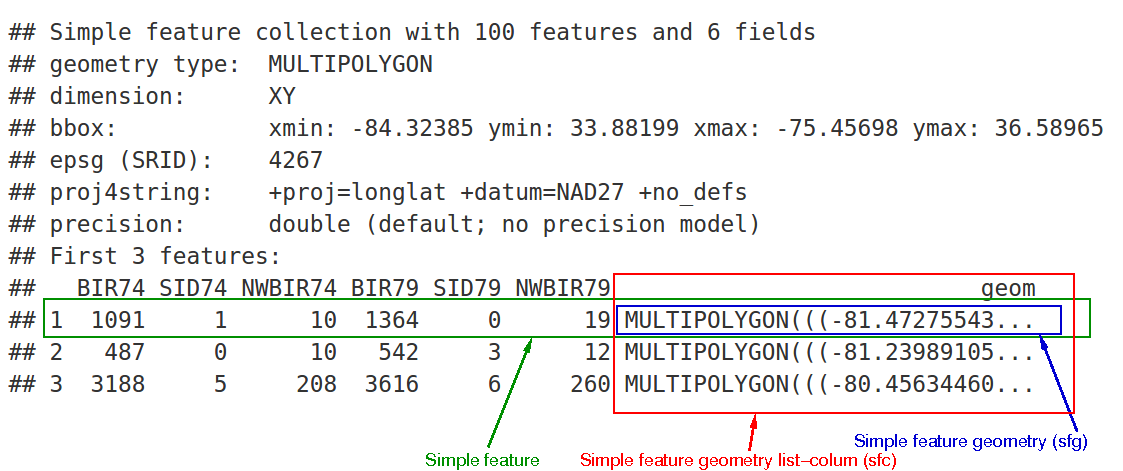
\includegraphics[width=15.6in]{img/sf} \end{center}

Les objets \texttt{sf} sont des \texttt{data.frame} dont l'une des
colonnes contient des géométries. Cette colonne est de la classe sfc
(simple feature column) et chaque individu de la colonne est un sfg
(simple feature geometry).\\
Ce format est très pratique dans la mesure ou les données et les
géométries sont intrinsèquement liées dans un même objet.

\subsection{Construction d'un objet sf}\label{construction-dun-objet-sf}

\textbf{Couche de points}

\begin{Shaded}
\begin{Highlighting}[]
\KeywordTok{library}\NormalTok{(sf)}
\NormalTok{pt1_sfg <-}\StringTok{ }\KeywordTok{st_point}\NormalTok{(}\KeywordTok{c}\NormalTok{(}\DecValTok{1}\NormalTok{,}\DecValTok{2}\NormalTok{))}
\NormalTok{pt2_sfg <-}\StringTok{ }\KeywordTok{st_point}\NormalTok{(}\KeywordTok{c}\NormalTok{(}\DecValTok{3}\NormalTok{,}\DecValTok{4}\NormalTok{))}
\NormalTok{pt3_sfg <-}\StringTok{ }\KeywordTok{st_point}\NormalTok{(}\KeywordTok{c}\NormalTok{(}\DecValTok{2}\NormalTok{,}\DecValTok{1}\NormalTok{))}
\NormalTok{(pt_sfc <-}\StringTok{ }\KeywordTok{st_sfc}\NormalTok{(pt1_sfg,pt2_sfg,pt3_sfg, }\DataTypeTok{crs =}\NormalTok{ (}\DecValTok{4326}\NormalTok{)))}
\end{Highlighting}
\end{Shaded}

\begin{verbatim}
Geometry set for 3 features 
geometry type:  POINT
dimension:      XY
bbox:           xmin: 1 ymin: 1 xmax: 3 ymax: 4
epsg (SRID):    4326
proj4string:    +proj=longlat +datum=WGS84 +no_defs
\end{verbatim}

\begin{Shaded}
\begin{Highlighting}[]
\NormalTok{pt_df <-}\StringTok{ }\KeywordTok{data.frame}\NormalTok{(}\DataTypeTok{id=} \KeywordTok{c}\NormalTok{(}\DecValTok{1}\NormalTok{,}\DecValTok{2}\NormalTok{,}\DecValTok{3}\NormalTok{), }\DataTypeTok{cat =} \KeywordTok{c}\NormalTok{(}\StringTok{"A"}\NormalTok{, }\StringTok{"B"}\NormalTok{, }\StringTok{"A"}\NormalTok{), }
                    \DataTypeTok{var1 =} \KeywordTok{c}\NormalTok{(}\DecValTok{10}\NormalTok{,}\DecValTok{20}\NormalTok{,}\DecValTok{30}\NormalTok{), }\DataTypeTok{var2 =} \KeywordTok{c}\NormalTok{(}\FloatTok{2.3}\NormalTok{,}\FloatTok{1.9}\NormalTok{,}\DecValTok{4}\NormalTok{))}
\NormalTok{(pt_sf <-}\StringTok{ }\KeywordTok{st_sf}\NormalTok{(pt_df,}\DataTypeTok{geometry =}\NormalTok{ pt_sfc))}
\end{Highlighting}
\end{Shaded}

\begin{verbatim}
Simple feature collection with 3 features and 4 fields
geometry type:  POINT
dimension:      XY
bbox:           xmin: 1 ymin: 1 xmax: 3 ymax: 4
epsg (SRID):    4326
proj4string:    +proj=longlat +datum=WGS84 +no_defs
  id cat var1 var2    geometry
1  1   A   10  2.3 POINT (1 2)
2  2   B   20  1.9 POINT (3 4)
3  3   A   30  4.0 POINT (2 1)
\end{verbatim}

\begin{Shaded}
\begin{Highlighting}[]
\KeywordTok{plot}\NormalTok{(pt_sf)}
\end{Highlighting}
\end{Shaded}

\begin{center}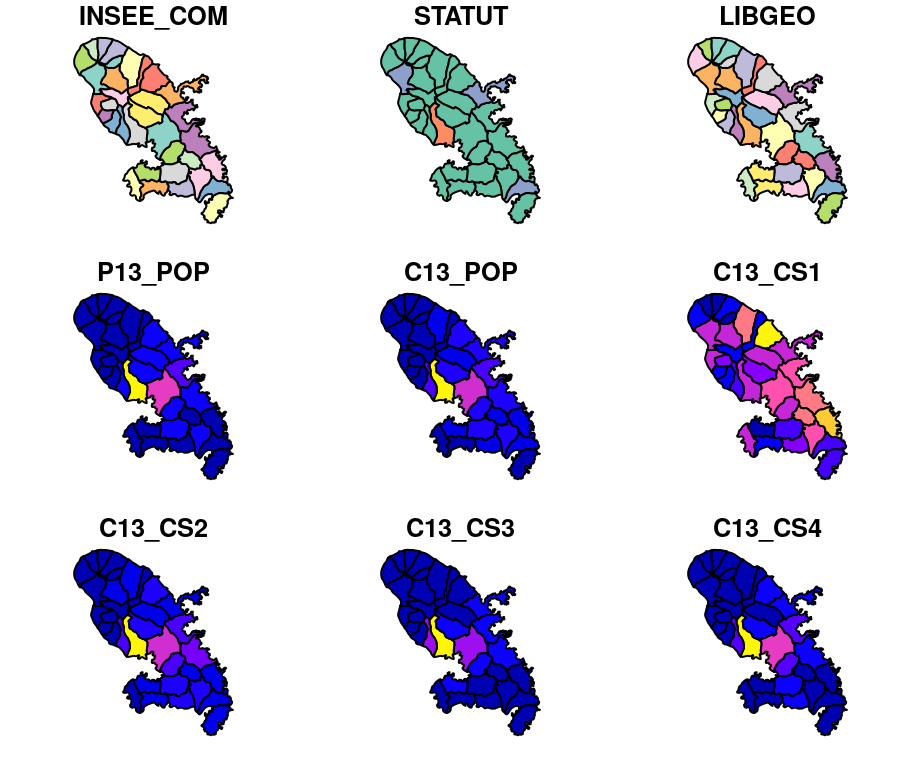
\includegraphics{Cartographie_avec_R_files/figure-latex/unnamed-chunk-2-1} \end{center}

\textbf{Couche de polygones}

\begin{Shaded}
\begin{Highlighting}[]
\NormalTok{p1 <-}\StringTok{ }\KeywordTok{rbind}\NormalTok{(}\KeywordTok{c}\NormalTok{(}\DecValTok{0}\NormalTok{,}\DecValTok{0}\NormalTok{), }\KeywordTok{c}\NormalTok{(}\DecValTok{1}\NormalTok{,}\DecValTok{0}\NormalTok{), }\KeywordTok{c}\NormalTok{(}\DecValTok{3}\NormalTok{,}\DecValTok{2}\NormalTok{), }\KeywordTok{c}\NormalTok{(}\DecValTok{2}\NormalTok{,}\DecValTok{4}\NormalTok{), }\KeywordTok{c}\NormalTok{(}\DecValTok{1}\NormalTok{,}\DecValTok{4}\NormalTok{), }\KeywordTok{c}\NormalTok{(}\DecValTok{0}\NormalTok{,}\DecValTok{0}\NormalTok{))}
\NormalTok{p2 <-}\StringTok{ }\KeywordTok{rbind}\NormalTok{(}\KeywordTok{c}\NormalTok{(}\DecValTok{3}\NormalTok{,}\DecValTok{0}\NormalTok{), }\KeywordTok{c}\NormalTok{(}\DecValTok{4}\NormalTok{,}\DecValTok{0}\NormalTok{), }\KeywordTok{c}\NormalTok{(}\DecValTok{4}\NormalTok{,}\DecValTok{1}\NormalTok{), }\KeywordTok{c}\NormalTok{(}\DecValTok{3}\NormalTok{,}\DecValTok{1}\NormalTok{), }\KeywordTok{c}\NormalTok{(}\DecValTok{3}\NormalTok{,}\DecValTok{0}\NormalTok{))}
\NormalTok{p3 <-}\StringTok{ }\KeywordTok{rbind}\NormalTok{(}\KeywordTok{c}\NormalTok{(}\DecValTok{3}\NormalTok{,}\DecValTok{3}\NormalTok{), }\KeywordTok{c}\NormalTok{(}\DecValTok{4}\NormalTok{,}\DecValTok{2}\NormalTok{), }\KeywordTok{c}\NormalTok{(}\DecValTok{4}\NormalTok{,}\DecValTok{3}\NormalTok{), }\KeywordTok{c}\NormalTok{(}\DecValTok{3}\NormalTok{,}\DecValTok{3}\NormalTok{))}
\NormalTok{pol1_sfg <-}\KeywordTok{st_polygon}\NormalTok{(}\KeywordTok{list}\NormalTok{(p1))}
\NormalTok{pol2_sfg <-}\KeywordTok{st_polygon}\NormalTok{(}\KeywordTok{list}\NormalTok{(p2))}
\NormalTok{pol3_sfg <-}\KeywordTok{st_polygon}\NormalTok{(}\KeywordTok{list}\NormalTok{(p3))}
\NormalTok{(pol_sfc <-}\StringTok{ }\KeywordTok{st_sfc}\NormalTok{(pol1_sfg, pol2_sfg, pol3_sfg, }\DataTypeTok{crs =} \DecValTok{4326}\NormalTok{))}
\end{Highlighting}
\end{Shaded}

\begin{verbatim}
Geometry set for 3 features 
geometry type:  POLYGON
dimension:      XY
bbox:           xmin: 0 ymin: 0 xmax: 4 ymax: 4
epsg (SRID):    4326
proj4string:    +proj=longlat +datum=WGS84 +no_defs
\end{verbatim}

\begin{Shaded}
\begin{Highlighting}[]
\NormalTok{pol_df <-}\StringTok{ }\KeywordTok{data.frame}\NormalTok{(}\DataTypeTok{id=} \KeywordTok{c}\NormalTok{(}\DecValTok{1}\NormalTok{,}\DecValTok{2}\NormalTok{,}\DecValTok{3}\NormalTok{), }\DataTypeTok{cat =} \KeywordTok{c}\NormalTok{(}\StringTok{"A"}\NormalTok{, }\StringTok{"B"}\NormalTok{, }\StringTok{"A"}\NormalTok{), }
                     \DataTypeTok{var1 =} \KeywordTok{c}\NormalTok{(}\DecValTok{10}\NormalTok{,}\DecValTok{20}\NormalTok{,}\DecValTok{30}\NormalTok{), }\DataTypeTok{var2 =} \KeywordTok{c}\NormalTok{(}\FloatTok{2.3}\NormalTok{,}\FloatTok{1.9}\NormalTok{,}\DecValTok{4}\NormalTok{))}
\NormalTok{(pol_sf <-}\StringTok{ }\KeywordTok{st_sf}\NormalTok{(pol_df,}\DataTypeTok{geometry =}\NormalTok{ pol_sfc))}
\end{Highlighting}
\end{Shaded}

\begin{verbatim}
Simple feature collection with 3 features and 4 fields
geometry type:  POLYGON
dimension:      XY
bbox:           xmin: 0 ymin: 0 xmax: 4 ymax: 4
epsg (SRID):    4326
proj4string:    +proj=longlat +datum=WGS84 +no_defs
  id cat var1 var2                       geometry
1  1   A   10  2.3 POLYGON ((0 0, 1 0, 3 2, 2 ...
2  2   B   20  1.9 POLYGON ((3 0, 4 0, 4 1, 3 ...
3  3   A   30  4.0 POLYGON ((3 3, 4 2, 4 3, 3 3))
\end{verbatim}

\begin{Shaded}
\begin{Highlighting}[]
\KeywordTok{plot}\NormalTok{(pol_sf)}
\end{Highlighting}
\end{Shaded}

\begin{center}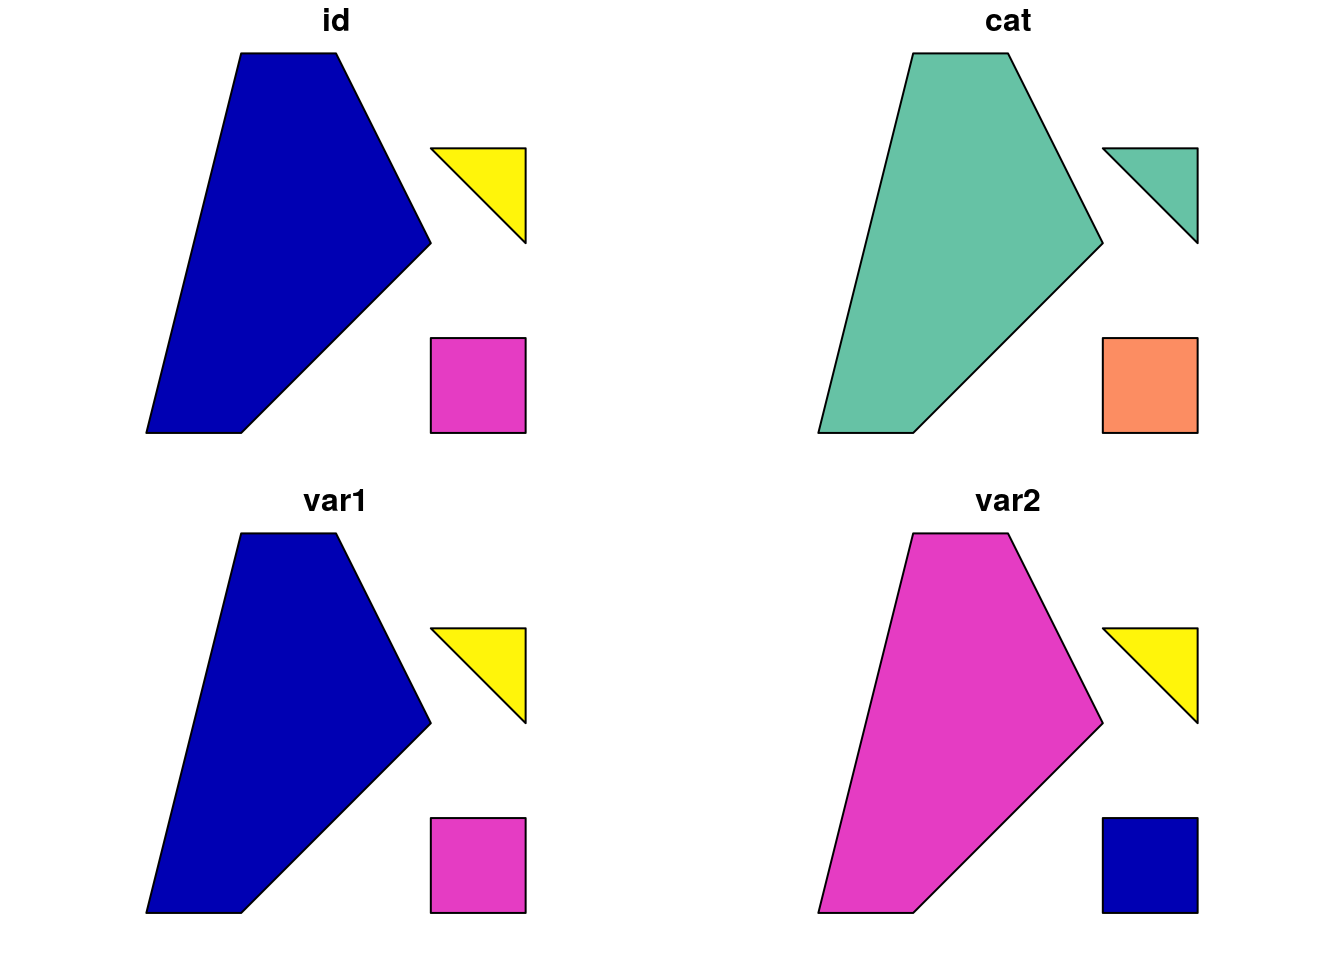
\includegraphics{Cartographie_avec_R_files/figure-latex/unnamed-chunk-3-1} \end{center}

\textbf{Couche de linestring}

\begin{Shaded}
\begin{Highlighting}[]
\NormalTok{p1 <-}\StringTok{ }\KeywordTok{rbind}\NormalTok{(}\KeywordTok{c}\NormalTok{(}\DecValTok{0}\NormalTok{,}\DecValTok{0}\NormalTok{), }\KeywordTok{c}\NormalTok{(}\DecValTok{1}\NormalTok{,}\DecValTok{0}\NormalTok{), }\KeywordTok{c}\NormalTok{(}\DecValTok{3}\NormalTok{,}\DecValTok{2}\NormalTok{), }\KeywordTok{c}\NormalTok{(}\DecValTok{2}\NormalTok{,}\DecValTok{4}\NormalTok{), }\KeywordTok{c}\NormalTok{(}\DecValTok{1}\NormalTok{,}\DecValTok{4}\NormalTok{))}
\NormalTok{p2 <-}\StringTok{ }\KeywordTok{rbind}\NormalTok{(}\KeywordTok{c}\NormalTok{(}\DecValTok{3}\NormalTok{,}\DecValTok{0}\NormalTok{), }\KeywordTok{c}\NormalTok{(}\DecValTok{4}\NormalTok{,}\DecValTok{0}\NormalTok{), }\KeywordTok{c}\NormalTok{(}\DecValTok{4}\NormalTok{,}\DecValTok{1}\NormalTok{), }\KeywordTok{c}\NormalTok{(}\DecValTok{3}\NormalTok{,}\DecValTok{1}\NormalTok{))}
\NormalTok{p3 <-}\StringTok{ }\KeywordTok{rbind}\NormalTok{(}\KeywordTok{c}\NormalTok{(}\DecValTok{3}\NormalTok{,}\DecValTok{3}\NormalTok{), }\KeywordTok{c}\NormalTok{(}\DecValTok{4}\NormalTok{,}\DecValTok{2}\NormalTok{), }\KeywordTok{c}\NormalTok{(}\DecValTok{4}\NormalTok{,}\DecValTok{3}\NormalTok{))}
\NormalTok{ls1_sfg <-}\KeywordTok{st_linestring}\NormalTok{(p1)}
\NormalTok{ls2_sfg <-}\KeywordTok{st_linestring}\NormalTok{(p2)}
\NormalTok{ls3_sfg <-}\KeywordTok{st_linestring}\NormalTok{(p3)}
\NormalTok{(ls_sfc <-}\StringTok{ }\KeywordTok{st_sfc}\NormalTok{(ls1_sfg, ls2_sfg, ls3_sfg, }\DataTypeTok{crs =} \DecValTok{4326}\NormalTok{))}
\end{Highlighting}
\end{Shaded}

\begin{verbatim}
Geometry set for 3 features 
geometry type:  LINESTRING
dimension:      XY
bbox:           xmin: 0 ymin: 0 xmax: 4 ymax: 4
epsg (SRID):    4326
proj4string:    +proj=longlat +datum=WGS84 +no_defs
\end{verbatim}

\begin{Shaded}
\begin{Highlighting}[]
\NormalTok{ls_df <-}\StringTok{ }\KeywordTok{data.frame}\NormalTok{(}\DataTypeTok{id=} \KeywordTok{c}\NormalTok{(}\DecValTok{1}\NormalTok{,}\DecValTok{2}\NormalTok{,}\DecValTok{3}\NormalTok{), }\DataTypeTok{cat =} \KeywordTok{c}\NormalTok{(}\StringTok{"A"}\NormalTok{, }\StringTok{"B"}\NormalTok{, }\StringTok{"A"}\NormalTok{), }
                    \DataTypeTok{var1 =} \KeywordTok{c}\NormalTok{(}\DecValTok{10}\NormalTok{,}\DecValTok{20}\NormalTok{,}\DecValTok{30}\NormalTok{), }\DataTypeTok{var2 =} \KeywordTok{c}\NormalTok{(}\FloatTok{2.3}\NormalTok{,}\FloatTok{1.9}\NormalTok{,}\DecValTok{4}\NormalTok{))}
\NormalTok{(ls_sf <-}\StringTok{ }\KeywordTok{st_sf}\NormalTok{(ls_df,}\DataTypeTok{geometry =}\NormalTok{ ls_sfc))}
\end{Highlighting}
\end{Shaded}

\begin{verbatim}
Simple feature collection with 3 features and 4 fields
geometry type:  LINESTRING
dimension:      XY
bbox:           xmin: 0 ymin: 0 xmax: 4 ymax: 4
epsg (SRID):    4326
proj4string:    +proj=longlat +datum=WGS84 +no_defs
  id cat var1 var2                       geometry
1  1   A   10  2.3 LINESTRING (0 0, 1 0, 3 2, ...
2  2   B   20  1.9 LINESTRING (3 0, 4 0, 4 1, ...
3  3   A   30  4.0     LINESTRING (3 3, 4 2, 4 3)
\end{verbatim}

\begin{Shaded}
\begin{Highlighting}[]
\KeywordTok{plot}\NormalTok{(ls_sf)}
\end{Highlighting}
\end{Shaded}

\begin{center}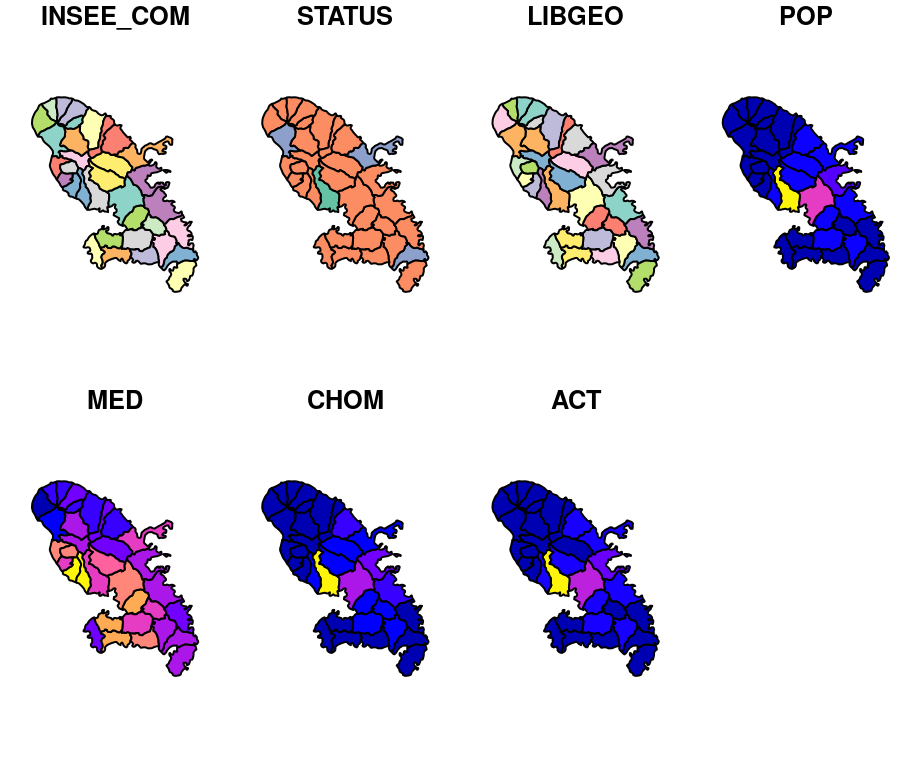
\includegraphics{Cartographie_avec_R_files/figure-latex/unnamed-chunk-4-1} \end{center}

\subsection{Import / Export}\label{import-export}

Les fonctions \texttt{st\_read()} et \texttt{st\_write()} permettent
d'importer et d'exporter de nombreux types de fichiers.

\begin{Shaded}
\begin{Highlighting}[]
\KeywordTok{library}\NormalTok{(sf)}
\NormalTok{mtq <-}\StringTok{ }\KeywordTok{st_read}\NormalTok{(}\StringTok{"data/martinique.shp"}\NormalTok{, }\DataTypeTok{quiet=}\OtherTok{TRUE}\NormalTok{)}
\end{Highlighting}
\end{Shaded}

\begin{Shaded}
\begin{Highlighting}[]
\KeywordTok{st_write}\NormalTok{(}\DataTypeTok{obj =}\NormalTok{ mtq, }\DataTypeTok{dsn =} \StringTok{"data/mtq.gpkg"}\NormalTok{, }\DataTypeTok{layer =} \StringTok{"mtq"}\NormalTok{, }\DataTypeTok{delete_layer =} \OtherTok{TRUE}\NormalTok{)}
\end{Highlighting}
\end{Shaded}

\begin{verbatim}
Deleting layer `mtq' using driver `GPKG'
Updating layer `mtq' to data source `data/mtq.gpkg' using driver `GPKG'
features:       34
fields:         23
geometry type:  Polygon
\end{verbatim}

\begin{Shaded}
\begin{Highlighting}[]
\KeywordTok{st_write}\NormalTok{(}\DataTypeTok{obj =}\NormalTok{ mtq, }\StringTok{"data/mtq.shp"}\NormalTok{, }\DataTypeTok{delete_layer =} \OtherTok{TRUE}\NormalTok{)}
\end{Highlighting}
\end{Shaded}

\begin{verbatim}
Deleting layer `mtq' using driver `ESRI Shapefile'
Writing layer `mtq' to data source `data/mtq.shp' using driver `ESRI Shapefile'
features:       34
fields:         23
geometry type:  Polygon
\end{verbatim}

\subsection{Affichage de données}\label{affichage-de-donnees}

\textbf{Aperçu des variables} via les fonctions \texttt{head()} et
\texttt{plot()}.

\begin{Shaded}
\begin{Highlighting}[]
\KeywordTok{head}\NormalTok{(mtq)}
\end{Highlighting}
\end{Shaded}

\begin{verbatim}
Simple feature collection with 6 features and 23 fields
geometry type:  POLYGON
dimension:      XY
bbox:           xmin: 695444.4 ymin: 1598817 xmax: 717731.2 ymax: 1645182
epsg (SRID):    32620
proj4string:    +proj=utm +zone=20 +datum=WGS84 +units=m +no_defs
  INSEE_COM         STATUT            LIBGEO P13_POP  C13_POP   C13_CS1   C13_CS2
1     97201 Commune simple L'Ajoupa-Bouillon    1830 1481.801  9.780866  48.90433
2     97202 Commune simple Les Anses-d'Arlet    3929 3190.115 97.433459 170.50855
3     97203 Commune simple      Basse-Pointe    3565 2983.215 39.510829  98.77707
     C13_CS3  C13_CS4  C13_CS5  C13_CS6  C13_CS7  C13_CS8 P08_POP  C08_POP  C08_CS1
1   9.780866 102.6991 273.8642 288.5355 430.3581 317.8781    1691 1346.519 31.40569
2 109.612642 239.5239 560.2424 385.6741 746.5743 880.5453    3826 3067.742 49.00453
3  43.461911 181.7498 568.9559 565.0048 940.5055 545.2494    3804 3054.108 44.51803
    C08_CS2  C08_CS3  C08_CS4  C08_CS5  C08_CS6  C08_CS7  C08_CS8
1  43.18282 11.77713 145.2513 223.7655 251.2455 380.7940 259.0969
2 143.95079 65.33937 216.3534 600.3054 459.4174 558.8020 974.5694
3 106.84327 27.70011 186.0292 448.1481 620.2845 881.5853 738.9993
                        geometry
1 POLYGON ((699261.2 1637681,...
2 POLYGON ((709840 1599026, 7...
3 POLYGON ((706092.8 1642964,...
 [ reached 'max' / getOption("max.print") -- omitted 3 rows ]
\end{verbatim}

\begin{Shaded}
\begin{Highlighting}[]
\KeywordTok{plot}\NormalTok{(mtq)}
\end{Highlighting}
\end{Shaded}

\begin{center}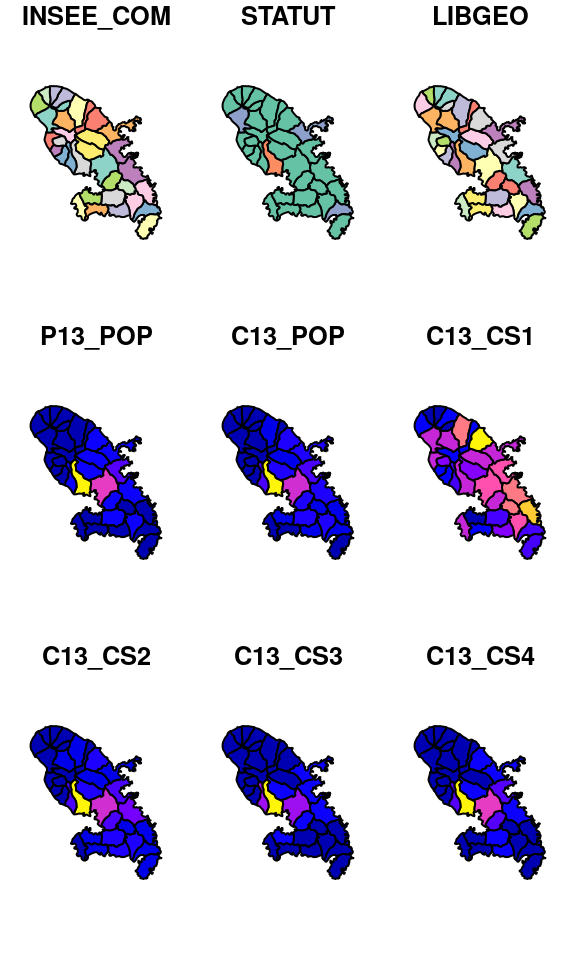
\includegraphics{Cartographie_avec_R_files/figure-latex/unnamed-chunk-5-1} \end{center}

\textbf{Affichage de la géométrie} uniquement.

\begin{Shaded}
\begin{Highlighting}[]
\KeywordTok{plot}\NormalTok{(}\KeywordTok{st_geometry}\NormalTok{(mtq))}
\end{Highlighting}
\end{Shaded}

\begin{center}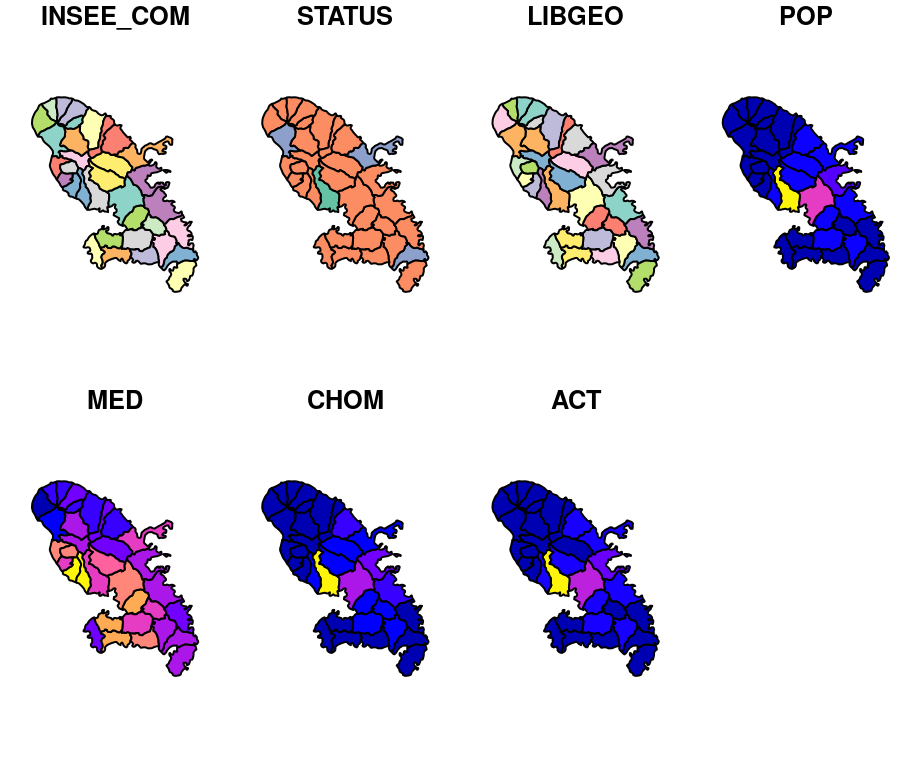
\includegraphics{Cartographie_avec_R_files/figure-latex/unnamed-chunk-6-1} \end{center}

\subsection{Joindre des données}\label{joindre-des-donnees}

On peut joindre un \texttt{data.frame} à un objet sf en utilisant la
fonction \texttt{merge()}.

\begin{Shaded}
\begin{Highlighting}[]
\NormalTok{mtq2016 <-}\StringTok{ }\KeywordTok{read.csv}\NormalTok{(}\DataTypeTok{file =} \StringTok{"data/mtq2016.csv"}\NormalTok{)}
\KeywordTok{head}\NormalTok{(mtq2016)}
\end{Highlighting}
\end{Shaded}

\begin{verbatim}
     ID                NOM Population.totale
1 97201 L' Ajoupa-Bouillon              1964
2 97202  Les Anses-d'Arlet              3686
3 97203       Basse-Pointe              3238
4 97234      Bellefontaine              1760
5 97204          Le Carbet              3655
6 97205        Case-Pilote              4522
\end{verbatim}

\begin{Shaded}
\begin{Highlighting}[]
\NormalTok{mtq <-}\StringTok{ }\KeywordTok{merge}\NormalTok{(}\DataTypeTok{x =}\NormalTok{ mtq, }\DataTypeTok{y =}\NormalTok{ mtq2016, }\DataTypeTok{by.x =} \StringTok{"INSEE_COM"}\NormalTok{, }\DataTypeTok{by.y =} \StringTok{"ID"}\NormalTok{)}
\KeywordTok{head}\NormalTok{(mtq)}
\end{Highlighting}
\end{Shaded}

\begin{verbatim}
Simple feature collection with 6 features and 25 fields
geometry type:  POLYGON
dimension:      XY
bbox:           xmin: 695444.4 ymin: 1598817 xmax: 717731.2 ymax: 1645182
epsg (SRID):    32620
proj4string:    +proj=utm +zone=20 +datum=WGS84 +units=m +no_defs
  INSEE_COM         STATUT            LIBGEO P13_POP  C13_POP   C13_CS1   C13_CS2
1     97201 Commune simple L'Ajoupa-Bouillon    1830 1481.801  9.780866  48.90433
2     97202 Commune simple Les Anses-d'Arlet    3929 3190.115 97.433459 170.50855
3     97203 Commune simple      Basse-Pointe    3565 2983.215 39.510829  98.77707
     C13_CS3  C13_CS4  C13_CS5  C13_CS6  C13_CS7  C13_CS8 P08_POP  C08_POP  C08_CS1
1   9.780866 102.6991 273.8642 288.5355 430.3581 317.8781    1691 1346.519 31.40569
2 109.612642 239.5239 560.2424 385.6741 746.5743 880.5453    3826 3067.742 49.00453
3  43.461911 181.7498 568.9559 565.0048 940.5055 545.2494    3804 3054.108 44.51803
    C08_CS2  C08_CS3  C08_CS4  C08_CS5  C08_CS6  C08_CS7  C08_CS8                NOM
1  43.18282 11.77713 145.2513 223.7655 251.2455 380.7940 259.0969 L' Ajoupa-Bouillon
2 143.95079 65.33937 216.3534 600.3054 459.4174 558.8020 974.5694  Les Anses-d'Arlet
3 106.84327 27.70011 186.0292 448.1481 620.2845 881.5853 738.9993       Basse-Pointe
  Population.totale                       geometry
1              1964 POLYGON ((699261.2 1637681,...
2              3686 POLYGON ((709840 1599026, 7...
3              3238 POLYGON ((706092.8 1642964,...
 [ reached 'max' / getOption("max.print") -- omitted 3 rows ]
\end{verbatim}

\section{Les systèmes de projections}\label{les-systemes-de-projections}

\subsection{Consulter la projection d'un
objet}\label{consulter-la-projection-dun-objet}

La fonction \texttt{st\_crs()} permet de consulter le système de
projection utilisé par un objet sf et de la modifier (\textbf{sans
reprojeter les données}).

\begin{Shaded}
\begin{Highlighting}[]
\KeywordTok{st_crs}\NormalTok{(mtq)}
\end{Highlighting}
\end{Shaded}

\begin{verbatim}
Coordinate Reference System:
  EPSG: 32620 
  proj4string: "+proj=utm +zone=20 +datum=WGS84 +units=m +no_defs"
\end{verbatim}

\subsection{Modifier la projection d'un
objet}\label{modifier-la-projection-dun-objet}

La fonction \texttt{st\_transform()} permet de reprojeter un objet sf.

\begin{Shaded}
\begin{Highlighting}[]
\KeywordTok{plot}\NormalTok{(}\KeywordTok{st_geometry}\NormalTok{(mtq))}
\KeywordTok{title}\NormalTok{(}\StringTok{"WGS 84 / UTM zone 20N"}\NormalTok{)}
\end{Highlighting}
\end{Shaded}

\begin{center}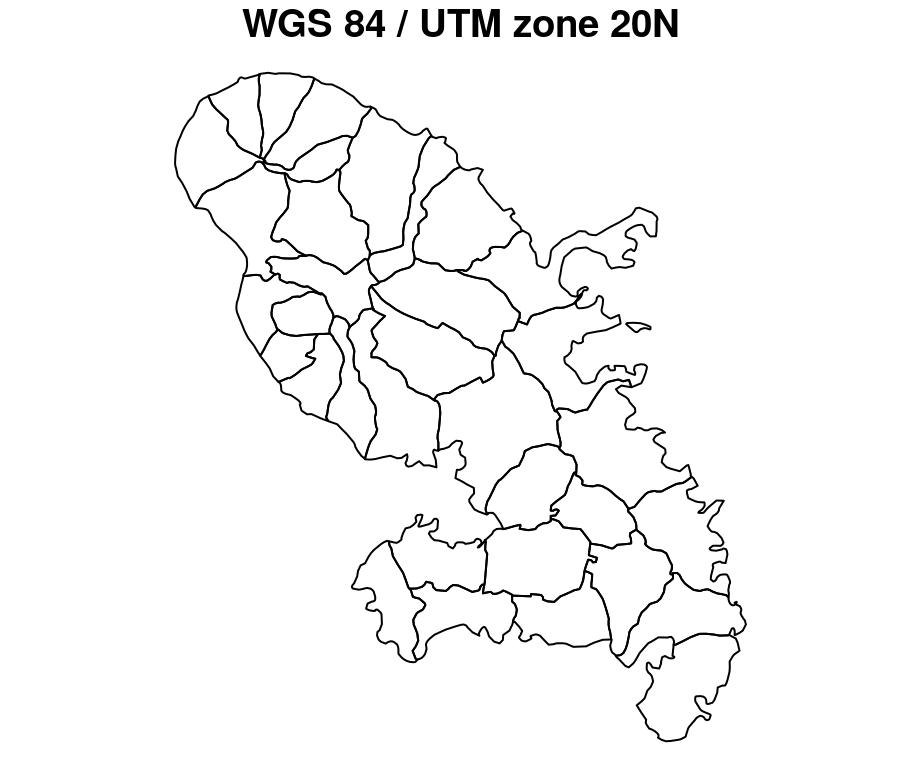
\includegraphics{Cartographie_avec_R_files/figure-latex/proj2-1} \end{center}

\begin{Shaded}
\begin{Highlighting}[]
\NormalTok{mtq_reproj <-}\StringTok{ }\KeywordTok{st_transform}\NormalTok{(mtq, }\DecValTok{2154}\NormalTok{)}
\KeywordTok{plot}\NormalTok{(}\KeywordTok{st_geometry}\NormalTok{(mtq_reproj))}
\KeywordTok{title}\NormalTok{(}\StringTok{"RGF93 / Lambert-93"}\NormalTok{)}
\end{Highlighting}
\end{Shaded}

\begin{center}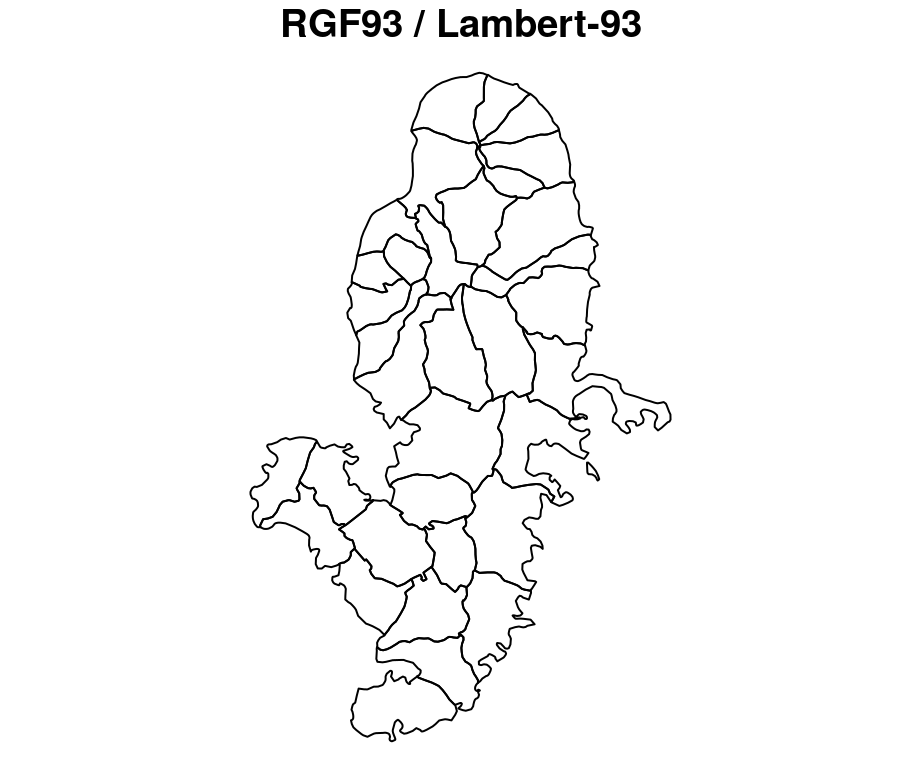
\includegraphics{Cartographie_avec_R_files/figure-latex/proj2-2} \end{center}

Le site \href{http://spatialreference.org/}{Spatial Reference} met à
disposition les références de très nombreux systèmes de projection.

\section{Opérations de géotraitement}\label{operations-de-geotraitement}

\subsection{Sélection par attributs}\label{selection-par-attributs}

Les objets \texttt{sf} \textbf{sont} des \texttt{data.frame}, on peut
donc sélectionner leur lignes et leur colonnes de la même manière que
les \texttt{data.frame}.

\begin{Shaded}
\begin{Highlighting}[]
\CommentTok{# selection de ligne}
\NormalTok{mtq[}\DecValTok{1}\OperatorTok{:}\DecValTok{2}\NormalTok{, ]}
\end{Highlighting}
\end{Shaded}

\begin{verbatim}
Simple feature collection with 2 features and 25 fields
geometry type:  POLYGON
dimension:      XY
bbox:           xmin: 697601.7 ymin: 1598817 xmax: 710461.9 ymax: 1640521
epsg (SRID):    32620
proj4string:    +proj=utm +zone=20 +datum=WGS84 +units=m +no_defs
  INSEE_COM         STATUT            LIBGEO P13_POP  C13_POP   C13_CS1   C13_CS2
1     97201 Commune simple L'Ajoupa-Bouillon    1830 1481.801  9.780866  48.90433
2     97202 Commune simple Les Anses-d'Arlet    3929 3190.115 97.433459 170.50855
     C13_CS3  C13_CS4  C13_CS5  C13_CS6  C13_CS7  C13_CS8 P08_POP  C08_POP  C08_CS1
1   9.780866 102.6991 273.8642 288.5355 430.3581 317.8781    1691 1346.519 31.40569
2 109.612642 239.5239 560.2424 385.6741 746.5743 880.5453    3826 3067.742 49.00453
    C08_CS2  C08_CS3  C08_CS4  C08_CS5  C08_CS6 C08_CS7  C08_CS8                NOM
1  43.18282 11.77713 145.2513 223.7655 251.2455 380.794 259.0969 L' Ajoupa-Bouillon
2 143.95079 65.33937 216.3534 600.3054 459.4174 558.802 974.5694  Les Anses-d'Arlet
  Population.totale                       geometry
1              1964 POLYGON ((699261.2 1637681,...
2              3686 POLYGON ((709840 1599026, 7...
\end{verbatim}

\begin{Shaded}
\begin{Highlighting}[]
\NormalTok{mtq[mtq}\OperatorTok{$}\NormalTok{LIBGEO}\OperatorTok{==}\StringTok{"Fort-de-France"}\NormalTok{, ]}
\end{Highlighting}
\end{Shaded}

\begin{verbatim}
Simple feature collection with 1 feature and 25 fields
geometry type:  POLYGON
dimension:      XY
bbox:           xmin: 704448.6 ymin: 1614283 xmax: 711650.9 ymax: 1626937
epsg (SRID):    32620
proj4string:    +proj=utm +zone=20 +datum=WGS84 +units=m +no_defs
  INSEE_COM               STATUT         LIBGEO P13_POP  C13_POP  C13_CS1  C13_CS2
9     97209 Préfecture de région Fort-de-France   84174 68712.33 86.57284 2720.489
   C13_CS3  C13_CS4  C13_CS5  C13_CS6  C13_CS7  C13_CS8 P08_POP  C08_POP  C08_CS1
9 4000.387 8407.424 13799.23 7309.136 16184.26 16204.84   89000 71566.82 119.0608
   C08_CS2  C08_CS3  C08_CS4 C08_CS5  C08_CS6  C08_CS7  C08_CS8            NOM
9 2480.105 3976.898 8630.605 15437.6 7964.513 15996.58 16961.46 Fort-de-France
  Population.totale                       geometry
9             82030 POLYGON ((711183.1 1619627,...
\end{verbatim}

\begin{Shaded}
\begin{Highlighting}[]
\CommentTok{# selection de colonnes}
\NormalTok{mtq[mtq}\OperatorTok{$}\NormalTok{LIBGEO}\OperatorTok{==}\StringTok{"Fort-de-France"}\NormalTok{, }\DecValTok{1}\OperatorTok{:}\DecValTok{4}\NormalTok{]}
\end{Highlighting}
\end{Shaded}

\begin{verbatim}
Simple feature collection with 1 feature and 4 fields
geometry type:  POLYGON
dimension:      XY
bbox:           xmin: 704448.6 ymin: 1614283 xmax: 711650.9 ymax: 1626937
epsg (SRID):    32620
proj4string:    +proj=utm +zone=20 +datum=WGS84 +units=m +no_defs
  INSEE_COM               STATUT         LIBGEO P13_POP                       geometry
9     97209 Préfecture de région Fort-de-France   84174 POLYGON ((711183.1 1619627,...
\end{verbatim}

\subsection{Sélection spatiale}\label{selection-spatiale}

Sélection des communes intesectant Fort-de-France

\begin{Shaded}
\begin{Highlighting}[]
\NormalTok{fdf <-}\StringTok{  }\NormalTok{mtq[mtq}\OperatorTok{$}\NormalTok{LIBGEO }\OperatorTok{==}\StringTok{ "Fort-de-France"}\NormalTok{, ]}
\NormalTok{mtq}\OperatorTok{$}\NormalTok{fdf <-}\StringTok{ }\KeywordTok{st_intersects}\NormalTok{(}\DataTypeTok{x =}\NormalTok{ mtq, }\DataTypeTok{y =}\NormalTok{ fdf, }\DataTypeTok{sparse =} \OtherTok{FALSE}\NormalTok{)}
\KeywordTok{plot}\NormalTok{(}\KeywordTok{st_geometry}\NormalTok{(mtq))}
\KeywordTok{plot}\NormalTok{(}\KeywordTok{st_geometry}\NormalTok{(mtq[mtq}\OperatorTok{$}\NormalTok{fdf,]), }\DataTypeTok{col =} \StringTok{"grey"}\NormalTok{, }\DataTypeTok{add =} \OtherTok{TRUE}\NormalTok{)}
\end{Highlighting}
\end{Shaded}

\begin{center}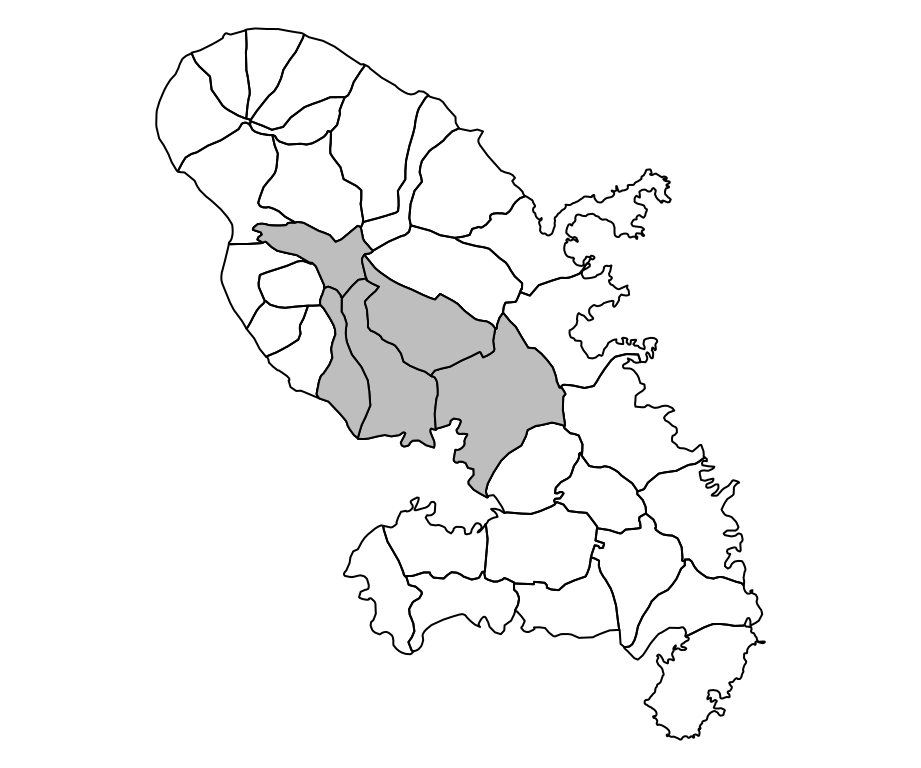
\includegraphics{Cartographie_avec_R_files/figure-latex/selectSpat-1} \end{center}

\subsection{Extraire des centroides}\label{extraire-des-centroides}

\begin{Shaded}
\begin{Highlighting}[]
\NormalTok{mtq_c <-}\StringTok{ }\KeywordTok{st_centroid}\NormalTok{(mtq)}
\KeywordTok{plot}\NormalTok{(}\KeywordTok{st_geometry}\NormalTok{(mtq))}
\KeywordTok{plot}\NormalTok{(}\KeywordTok{st_geometry}\NormalTok{(mtq_c), }\DataTypeTok{add=}\OtherTok{TRUE}\NormalTok{, }\DataTypeTok{cex=}\FloatTok{1.2}\NormalTok{, }\DataTypeTok{col=}\StringTok{"red"}\NormalTok{, }\DataTypeTok{pch=}\DecValTok{20}\NormalTok{)}
\end{Highlighting}
\end{Shaded}

\begin{center}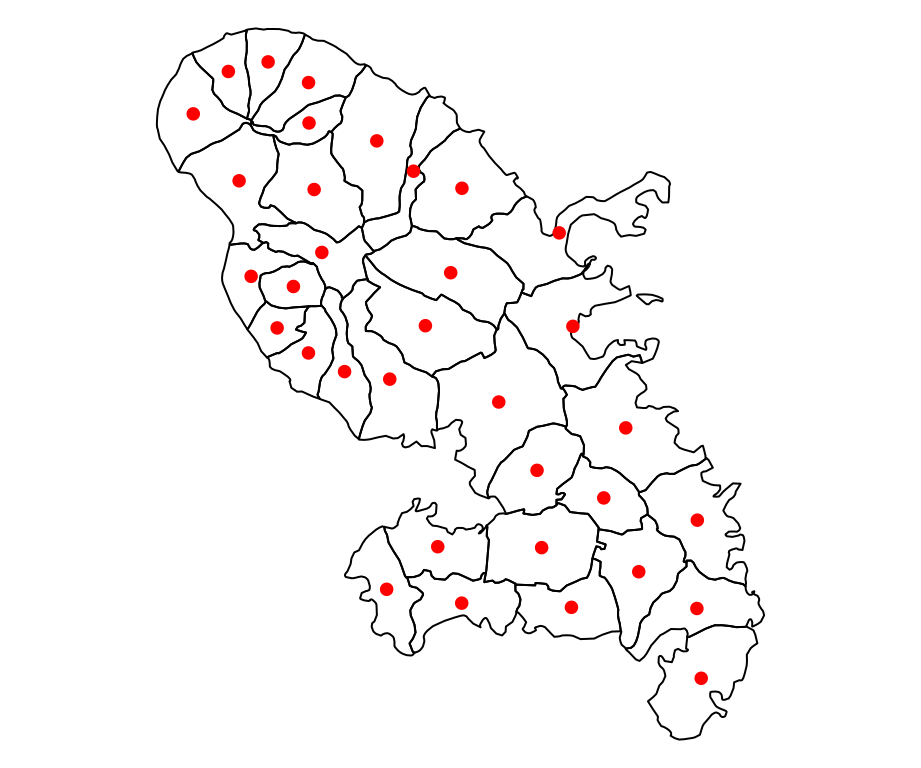
\includegraphics{Cartographie_avec_R_files/figure-latex/centroid-1} \end{center}

\subsection{Créer une matrice de
distances}\label{creer-une-matrice-de-distances}

Si le système de projection du jeu de données est renseigné les
distances sont exprimées dans l'unité de mesure de la projection (en
mètres le plus souvent).

\begin{Shaded}
\begin{Highlighting}[]
\NormalTok{mat <-}\StringTok{ }\KeywordTok{st_distance}\NormalTok{(}\DataTypeTok{x =}\NormalTok{ mtq_c, }\DataTypeTok{y =}\NormalTok{ mtq_c)}
\NormalTok{mat[}\DecValTok{1}\OperatorTok{:}\DecValTok{5}\NormalTok{,}\DecValTok{1}\OperatorTok{:}\DecValTok{5}\NormalTok{]}
\end{Highlighting}
\end{Shaded}

\begin{verbatim}
Units: [m]
          [,1]     [,2]      [,3]      [,4]      [,5]
[1,]     0.000 35297.56  3091.501 12131.617 17136.310
[2,] 35297.557     0.00 38332.602 25518.913 18605.249
[3,]  3091.501 38332.60     0.000 15094.702 20226.198
[4,] 12131.617 25518.91 15094.702     0.000  7177.011
[5,] 17136.310 18605.25 20226.198  7177.011     0.000
\end{verbatim}

\subsection{Agréger des polygones}\label{agreger-des-polygones}

\begin{Shaded}
\begin{Highlighting}[]
\NormalTok{mtq_u <-}\StringTok{ }\KeywordTok{st_union}\NormalTok{(mtq)}
\KeywordTok{plot}\NormalTok{(}\KeywordTok{st_geometry}\NormalTok{(mtq), }\DataTypeTok{col=}\StringTok{"lightblue"}\NormalTok{)}
\KeywordTok{plot}\NormalTok{(}\KeywordTok{st_geometry}\NormalTok{(mtq_u), }\DataTypeTok{add=}\NormalTok{T, }\DataTypeTok{lwd=}\DecValTok{2}\NormalTok{, }\DataTypeTok{border =} \StringTok{"red"}\NormalTok{)}
\end{Highlighting}
\end{Shaded}

\begin{center}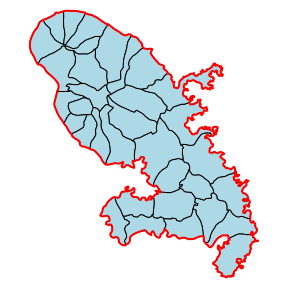
\includegraphics{Cartographie_avec_R_files/figure-latex/aggreg-1} \end{center}

\subsection{Agréger des polygones en fonction d'une
variable}\label{agreger-des-polygones-en-fonction-dune-variable}

\begin{Shaded}
\begin{Highlighting}[]
\KeywordTok{library}\NormalTok{(dplyr)}
\NormalTok{mtq_u2 <-}\StringTok{ }\NormalTok{mtq }\OperatorTok\StringTok{ }
\StringTok{  }\KeywordTok{group_by}\NormalTok{(STATUT) }\OperatorTok\StringTok{ }
\StringTok{  }\KeywordTok{summarize}\NormalTok{(}\DataTypeTok{P13_POP=}\KeywordTok{sum}\NormalTok{(P13_POP))}
\KeywordTok{plot}\NormalTok{(mtq_u2[}\StringTok{"STATUT"}\NormalTok{], }\DataTypeTok{key.pos =} \OtherTok{NULL}\NormalTok{)}
\end{Highlighting}
\end{Shaded}

\begin{center}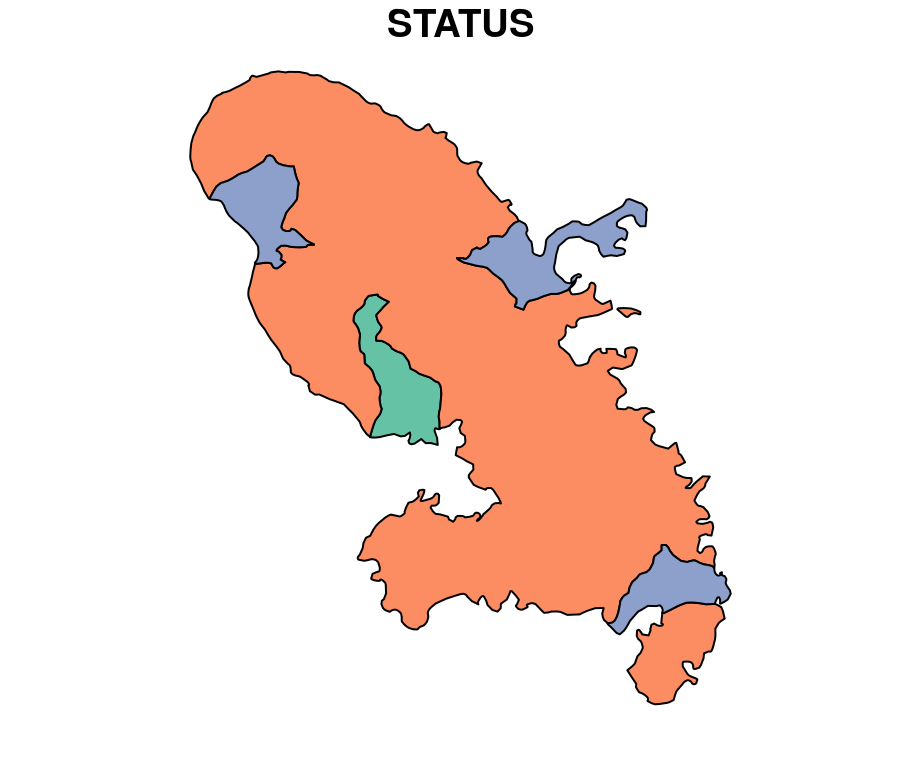
\includegraphics{Cartographie_avec_R_files/figure-latex/aggreg2-1} \end{center}

\subsection{Construire une zone
tampon}\label{construire-une-zone-tampon}

\begin{Shaded}
\begin{Highlighting}[]
\NormalTok{mtq_b <-}\StringTok{ }\KeywordTok{st_buffer}\NormalTok{(}\DataTypeTok{x =}\NormalTok{ mtq_u, }\DataTypeTok{dist =} \DecValTok{2000}\NormalTok{)}
\KeywordTok{plot}\NormalTok{(}\KeywordTok{st_geometry}\NormalTok{(mtq), }\DataTypeTok{col=}\StringTok{"lightblue"}\NormalTok{)}
\KeywordTok{plot}\NormalTok{(}\KeywordTok{st_geometry}\NormalTok{(mtq_u), }\DataTypeTok{add=}\NormalTok{T, }\DataTypeTok{lwd=}\DecValTok{2}\NormalTok{)}
\KeywordTok{plot}\NormalTok{(}\KeywordTok{st_geometry}\NormalTok{(mtq_b), }\DataTypeTok{add=}\NormalTok{T, }\DataTypeTok{lwd=}\DecValTok{2}\NormalTok{, }\DataTypeTok{border =} \StringTok{"red"}\NormalTok{)}
\end{Highlighting}
\end{Shaded}

\begin{center}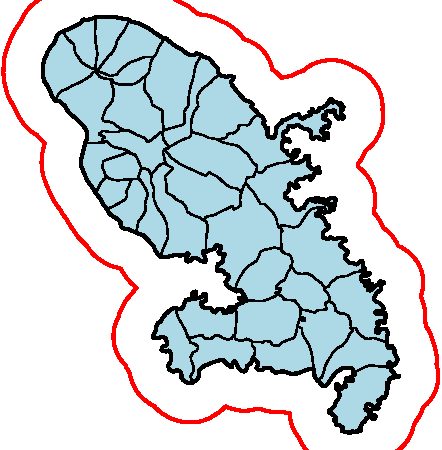
\includegraphics{Cartographie_avec_R_files/figure-latex/buffers-1} \end{center}

\subsection{Réaliser une intersection}\label{realiser-une-intersection}

\begin{Shaded}
\begin{Highlighting}[]
\NormalTok{m <-}\StringTok{ }\KeywordTok{rbind}\NormalTok{(}\KeywordTok{c}\NormalTok{(}\DecValTok{700015}\NormalTok{,}\DecValTok{1624212}\NormalTok{), }\KeywordTok{c}\NormalTok{(}\DecValTok{700015}\NormalTok{,}\DecValTok{1641586}\NormalTok{), }\KeywordTok{c}\NormalTok{(}\DecValTok{719127}\NormalTok{,}\DecValTok{1641586}\NormalTok{), }
           \KeywordTok{c}\NormalTok{(}\DecValTok{719127}\NormalTok{,}\DecValTok{1624212}\NormalTok{), }\KeywordTok{c}\NormalTok{(}\DecValTok{700015}\NormalTok{,}\DecValTok{1624212}\NormalTok{))}
\NormalTok{p <-}\StringTok{ }\KeywordTok{st_sf}\NormalTok{(}\KeywordTok{st_sfc}\NormalTok{(}\KeywordTok{st_polygon}\NormalTok{(}\KeywordTok{list}\NormalTok{(m))), }\DataTypeTok{crs =} \KeywordTok{st_crs}\NormalTok{(mtq))}
\KeywordTok{plot}\NormalTok{(}\KeywordTok{st_geometry}\NormalTok{(mtq))}
\KeywordTok{plot}\NormalTok{(p, }\DataTypeTok{border=}\StringTok{"red"}\NormalTok{, }\DataTypeTok{lwd=}\DecValTok{2}\NormalTok{, }\DataTypeTok{add=}\NormalTok{T)}
\end{Highlighting}
\end{Shaded}

\begin{center}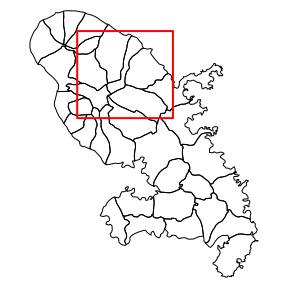
\includegraphics{Cartographie_avec_R_files/figure-latex/intersect-1} \end{center}

\begin{Shaded}
\begin{Highlighting}[]
\NormalTok{mtq_z <-}\StringTok{ }\KeywordTok{st_intersection}\NormalTok{(}\DataTypeTok{x =}\NormalTok{ mtq, }\DataTypeTok{y =}\NormalTok{ p)}
\KeywordTok{plot}\NormalTok{(}\KeywordTok{st_geometry}\NormalTok{(mtq))}
\KeywordTok{plot}\NormalTok{(}\KeywordTok{st_geometry}\NormalTok{(mtq_z), }\DataTypeTok{col=}\StringTok{"red"}\NormalTok{, }\DataTypeTok{border=}\StringTok{"green"}\NormalTok{, }\DataTypeTok{add=}\NormalTok{T)}
\end{Highlighting}
\end{Shaded}

\begin{center}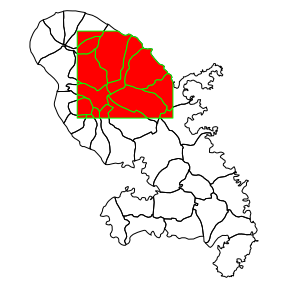
\includegraphics{Cartographie_avec_R_files/figure-latex/intersect-2} \end{center}

\begin{Shaded}
\begin{Highlighting}[]
\KeywordTok{plot}\NormalTok{(}\KeywordTok{st_geometry}\NormalTok{(mtq_z))}
\end{Highlighting}
\end{Shaded}

\begin{center}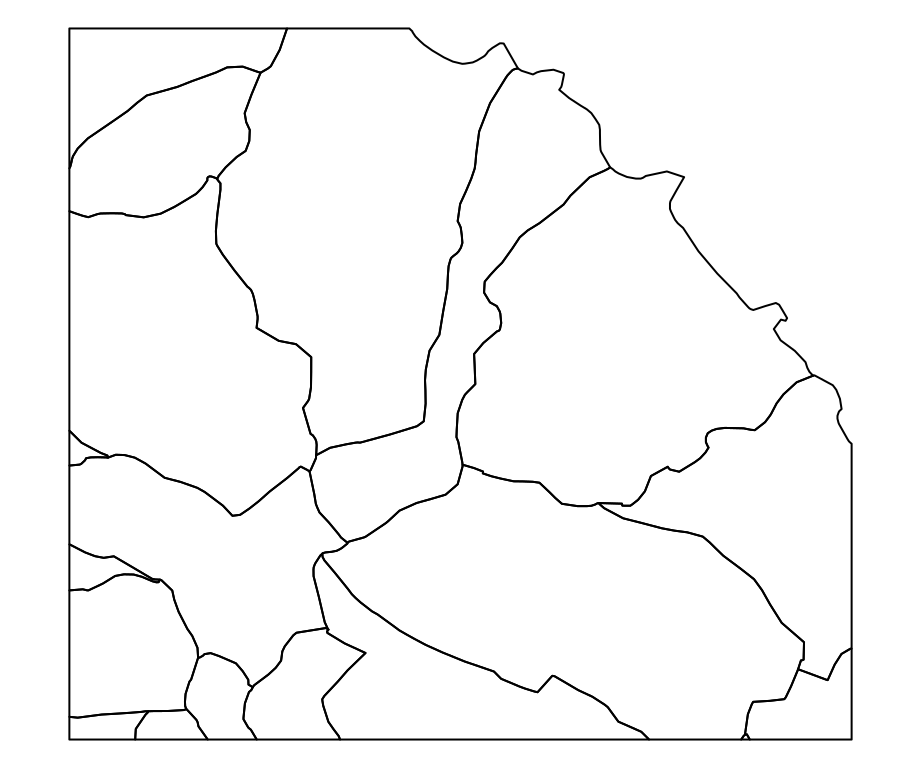
\includegraphics{Cartographie_avec_R_files/figure-latex/intersect-3} \end{center}

\subsection{Compter des points dans un
polygone}\label{compter-des-points-dans-un-polygone}

\begin{Shaded}
\begin{Highlighting}[]
\NormalTok{pts <-}\StringTok{ }\KeywordTok{st_sample}\NormalTok{(}\DataTypeTok{x =}\NormalTok{ mtq, }\DataTypeTok{size =} \DecValTok{50}\NormalTok{)}
\KeywordTok{plot}\NormalTok{(}\KeywordTok{st_geometry}\NormalTok{(mtq))}
\KeywordTok{plot}\NormalTok{(pts, }\DataTypeTok{pch =} \DecValTok{20}\NormalTok{, }\DataTypeTok{col =} \StringTok{"red"}\NormalTok{, }\DataTypeTok{add=}\OtherTok{TRUE}\NormalTok{, }\DataTypeTok{cex =} \DecValTok{1}\NormalTok{)}
\end{Highlighting}
\end{Shaded}

\begin{center}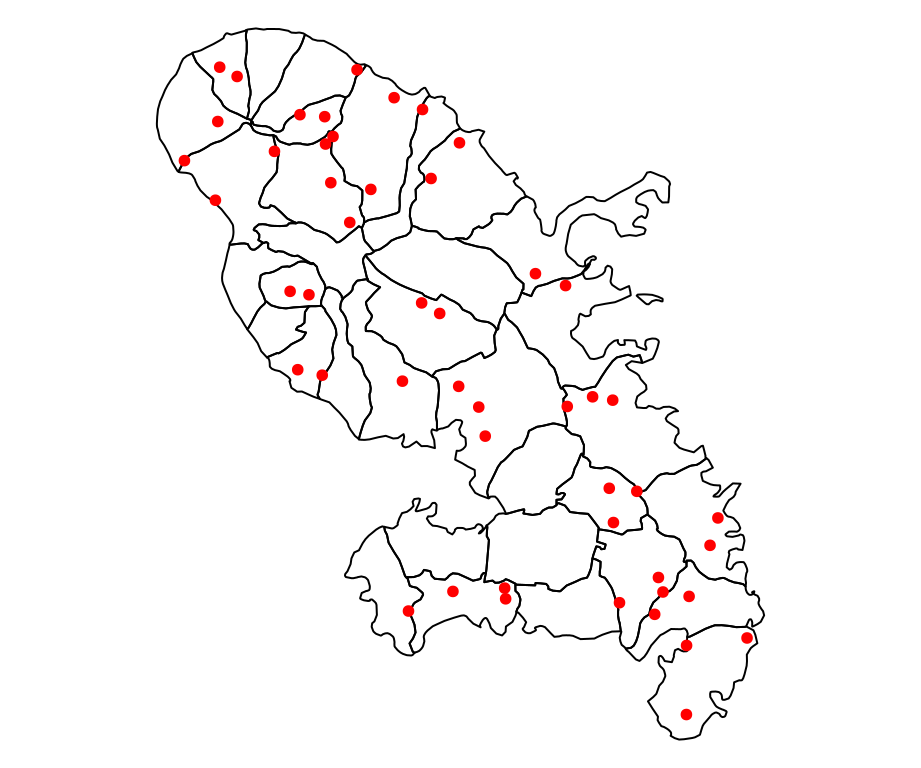
\includegraphics{Cartographie_avec_R_files/figure-latex/intersect2-1} \end{center}

\begin{Shaded}
\begin{Highlighting}[]
\NormalTok{inter <-}\StringTok{ }\KeywordTok{st_intersects}\NormalTok{(mtq, pts)}
\NormalTok{mtq}\OperatorTok{$}\NormalTok{nbpts <-}\StringTok{ }\KeywordTok{sapply}\NormalTok{(}\DataTypeTok{X =}\NormalTok{ inter, }\DataTypeTok{FUN =}\NormalTok{ length)}
\KeywordTok{plot}\NormalTok{(}\KeywordTok{st_geometry}\NormalTok{(mtq))}
\KeywordTok{plot}\NormalTok{(}\KeywordTok{st_geometry}\NormalTok{(mtq[mtq}\OperatorTok{$}\NormalTok{nbpts}\OperatorTok{>}\DecValTok{2}\NormalTok{,]), }\DataTypeTok{col =} \StringTok{"grey"}\NormalTok{, }\DataTypeTok{add=}\OtherTok{TRUE}\NormalTok{)}
\KeywordTok{plot}\NormalTok{(pts, }\DataTypeTok{pch =} \DecValTok{20}\NormalTok{, }\DataTypeTok{col =} \StringTok{"red"}\NormalTok{, }\DataTypeTok{add=}\OtherTok{TRUE}\NormalTok{, }\DataTypeTok{cex =} \DecValTok{1}\NormalTok{)}
\end{Highlighting}
\end{Shaded}

\begin{center}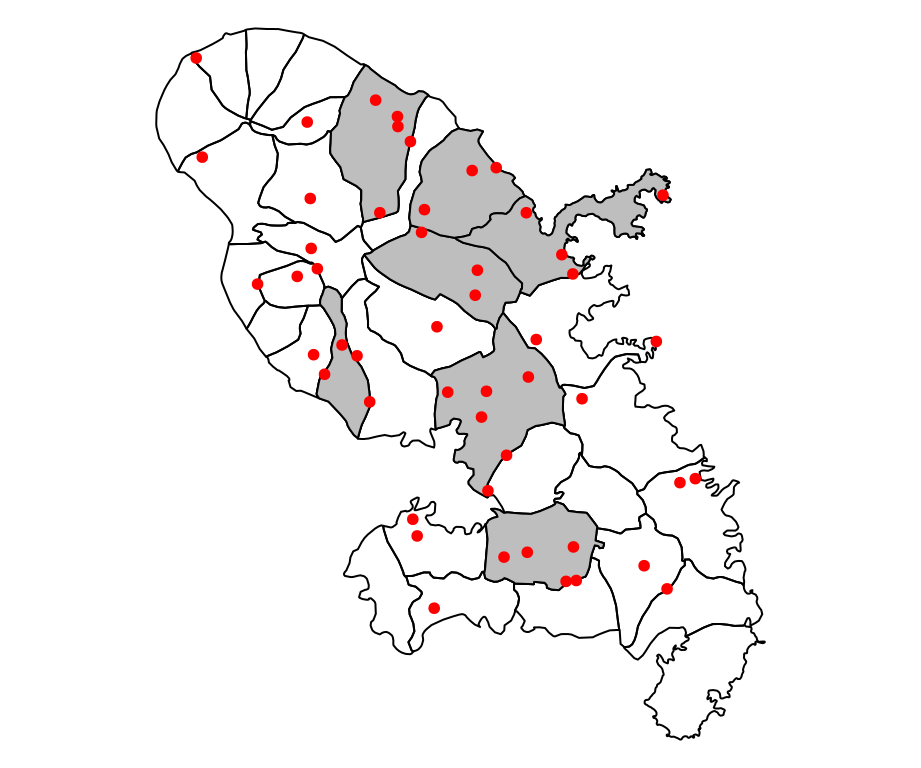
\includegraphics{Cartographie_avec_R_files/figure-latex/intersect2-2} \end{center}

\subsection{Construire des polygones de
Voronoi}\label{construire-des-polygones-de-voronoi}

google: ``st\_voronoi R sf''
(\url{https://github.com/r-spatial/sf/issues/474} \&
\url{https://stackoverflow.com/questions/45719790/create-voronoi-polygon-with-simple-feature-in-r})

\begin{Shaded}
\begin{Highlighting}[]
\NormalTok{mtq_v <-}\StringTok{ }\KeywordTok{st_voronoi}\NormalTok{(}\DataTypeTok{x =} \KeywordTok{st_union}\NormalTok{(mtq_c))}
\NormalTok{mtq_v <-}\StringTok{ }\KeywordTok{st_intersection}\NormalTok{(}\KeywordTok{st_cast}\NormalTok{(mtq_v), }\KeywordTok{st_union}\NormalTok{(mtq))}
\NormalTok{mtq_v <-}\StringTok{ }\KeywordTok{st_join}\NormalTok{(}\DataTypeTok{x =} \KeywordTok{st_sf}\NormalTok{(mtq_v), }\DataTypeTok{y =}\NormalTok{ mtq_c, }\DataTypeTok{join=}\NormalTok{st_intersects)}
\NormalTok{mtq_v <-}\StringTok{ }\KeywordTok{st_cast}\NormalTok{(mtq_v, }\StringTok{"MULTIPOLYGON"}\NormalTok{)}
\KeywordTok{plot}\NormalTok{(}\KeywordTok{st_geometry}\NormalTok{(mtq_v), }\DataTypeTok{col=}\StringTok{'lightblue'}\NormalTok{)}
\end{Highlighting}
\end{Shaded}

\begin{center}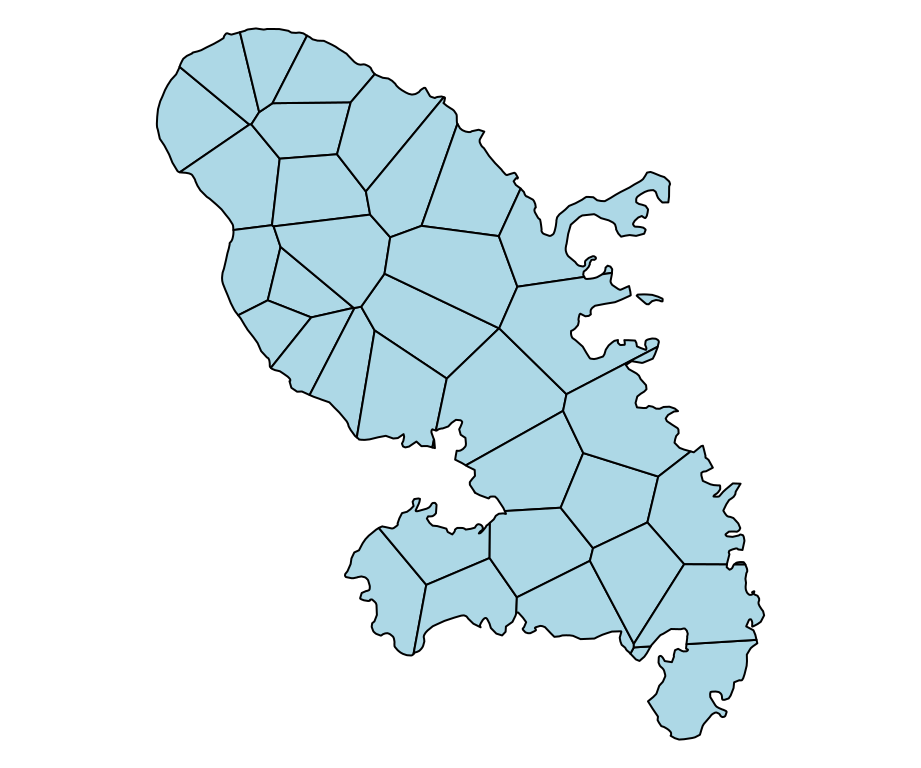
\includegraphics{Cartographie_avec_R_files/figure-latex/voronoi-1} \end{center}

\section{Géocodage d'adresses}\label{geocodage-dadresses}

Plusieurs packages permettent de géocoder des adresses.

\begin{itemize}
\tightlist
\item
  \texttt{photon} \citep{R-photon}
\end{itemize}

\begin{Shaded}
\begin{Highlighting}[]
\CommentTok{# remotes::install_github(repo = 'rCarto/photon')  }
\KeywordTok{library}\NormalTok{(photon)}
\NormalTok{address <-}\StringTok{ }\KeywordTok{c}\NormalTok{(}\StringTok{"19 rue Michel Bakounine, 29600 Morlaix, France"}\NormalTok{,}
             \StringTok{"8 place Paul Ricoeur, 75013 Paris"}\NormalTok{)}
\NormalTok{place <-}\StringTok{ }\NormalTok{photon}\OperatorTok{::}\KeywordTok{geocode}\NormalTok{(address, }\DataTypeTok{limit =} \DecValTok{1}\NormalTok{, }\DataTypeTok{key =} \StringTok{"place"}\NormalTok{, }\DataTypeTok{lang =} \StringTok{"fr"}\NormalTok{)}
\NormalTok{place}
\end{Highlighting}
\end{Shaded}

\begin{verbatim}
                                        location     osm_id osm_type name housenumber
1 19 rue Michel Bakounine, 29600 Morlaix, France 3241060871        N <NA>          19
2              8 place Paul Ricoeur, 75013 Paris 2608793979        N <NA>           8
                street postcode    city         state country osm_key osm_value       lon
1 Rue Michel Bakounine    29600 Morlaix      Bretagne  France   place     house -3.816435
2   Place Paul Ricoeur    75013   Paris Île-de-France  France   place     house  2.382483
       lat  msg
1 48.59041 <NA>
2 48.82670 <NA>
\end{verbatim}

\begin{itemize}
\tightlist
\item
  \texttt{nominatim} \citep{R-nominatim}
\end{itemize}

\begin{Shaded}
\begin{Highlighting}[]
\CommentTok{# remotes::install_github("hrbrmstr/nominatim")}
\KeywordTok{library}\NormalTok{(nominatim)}
\NormalTok{address <-}\StringTok{ }\KeywordTok{c}\NormalTok{(}\KeywordTok{URLencode}\NormalTok{(}\StringTok{"19 rue Michel Bakounine, 29600 Morlaix, France"}\NormalTok{),}
             \KeywordTok{URLencode}\NormalTok{(}\StringTok{"8 place Paul Ricoeur, 75013 Paris"}\NormalTok{))}
\NormalTok{place <-}\StringTok{ }\KeywordTok{osm_geocode}\NormalTok{(address, }
                     \DataTypeTok{country_codes =} \StringTok{"FR"}\NormalTok{, }
                     \DataTypeTok{key =} \StringTok{"UneClefMapQuestValide"}\NormalTok{)}
\NormalTok{place}
\end{Highlighting}
\end{Shaded}

\begin{verbatim}
  place_id
1 44644129
2 27209988
                                                                               licence
1 Data © OpenStreetMap contributors, ODbL 1.0. https://www.openstreetmap.org/copyright
2 Data © OpenStreetMap contributors, ODbL 1.0. https://www.openstreetmap.org/copyright
  osm_type     osm_id      lat       lon
1     node 3241060871 48.59041 -3.816435
2     node 2608793979 48.82670  2.382483
                                                                                                   display_name
1 19, Rue Michel Bakounine, Ploujean, Kerozar, Morlaix, Finistère, Brittany, Metropolitan France, 29600, France
2    8, Place Paul Ricoeur, Gare, 13th Arrondissement, Paris, Ile-de-France, Metropolitan France, 75013, France
  class  type importance bbox_left bbox_top bbox_right bbox_bottom
1 place house      0.741  48.59036 48.59046  -3.816485   -3.816384
2 place house      0.631  48.82665 48.82675   2.382433    2.382533
\end{verbatim}

\begin{itemize}
\tightlist
\item
  \texttt{banR} \citep{R-banR}, pour des adresses en France uniquement.
\end{itemize}

\begin{Shaded}
\begin{Highlighting}[]
\KeywordTok{library}\NormalTok{(banR)}
\NormalTok{address <-}\StringTok{ }\KeywordTok{c}\NormalTok{(}\StringTok{"19 rue Michel Bakounine, 29600 Morlaix, France"}\NormalTok{,}
             \StringTok{"8 place Paul Ricoeur, 75013 Paris"}\NormalTok{)}
\NormalTok{place <-}\StringTok{ }\KeywordTok{geocode_tbl}\NormalTok{(}\DataTypeTok{tbl =} \KeywordTok{data.frame}\NormalTok{(address), }\DataTypeTok{adresse =} \StringTok{"address"}\NormalTok{)}
\NormalTok{place}
\end{Highlighting}
\end{Shaded}

\begin{verbatim}
# A tibble: 2 x 14
  address latitude longitude result_label result_score result_type result_id
  <chr>      <dbl>     <dbl> <chr>               <dbl> <chr>       <chr>    
1 19 rue~     48.6     -3.82 19 Rue Mich~         0.78 housenumber ADRNIVX_~
2 8 plac~     48.8      2.38 8 Place Pau~         0.93 housenumber ADRNIVX_~
# ... with 7 more variables: result_housenumber <int>, result_name <chr>,
#   result_street <chr>, result_postcode <int>, result_city <chr>, result_context <chr>,
#   result_citycode <chr>
\end{verbatim}

\textbf{Transformer les données en objet \texttt{sf}}

\begin{Shaded}
\begin{Highlighting}[]
\KeywordTok{library}\NormalTok{(sf)}
\KeywordTok{library}\NormalTok{(cartography)}
\NormalTok{place_sf <-}\StringTok{ }\KeywordTok{st_as_sf}\NormalTok{(place, }\DataTypeTok{coords =} \KeywordTok{c}\NormalTok{(}\StringTok{"longitude"}\NormalTok{, }\StringTok{"latitude"}\NormalTok{), }\DataTypeTok{crs =} \DecValTok{4326}\NormalTok{)}
\NormalTok{osm_fr <-}\StringTok{ }\KeywordTok{getTiles}\NormalTok{(}\DataTypeTok{x =}\NormalTok{ place_sf, }\DataTypeTok{zoom =} \DecValTok{7}\NormalTok{ )}
\KeywordTok{tilesLayer}\NormalTok{(osm_fr)}
\KeywordTok{plot}\NormalTok{(}\KeywordTok{st_geometry}\NormalTok{(place_sf), }\DataTypeTok{pch =} \DecValTok{20}\NormalTok{, }\DataTypeTok{cex =} \DecValTok{4}\NormalTok{, }\DataTypeTok{col =} \StringTok{"red"}\NormalTok{, }\DataTypeTok{add=}\NormalTok{T)}
\end{Highlighting}
\end{Shaded}

\begin{center}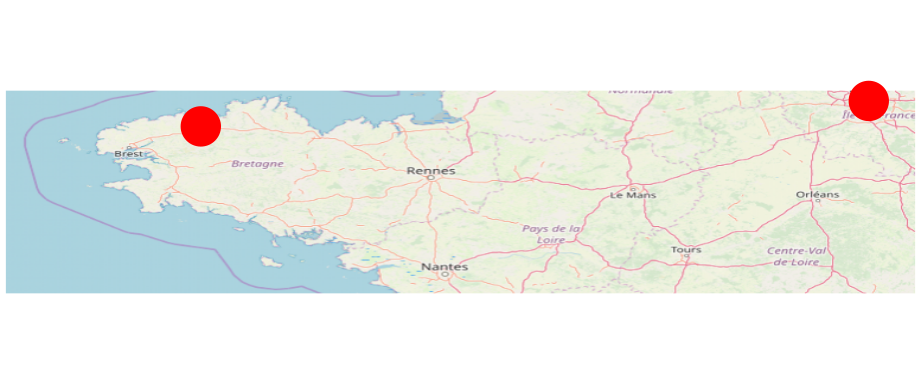
\includegraphics{Cartographie_avec_R_files/figure-latex/adddisplay-1} \end{center}

\section{Importer des données OSM}\label{importer-des-donnees-osm}

\href{https://www.openstreetmap.org}{OpenStreetMap (OSM)} est un projet
de cartographie participative qui a pour but de constituer une base de
données géographiques libre à l'échelle mondiale. OpenStreetMap vous
permet de voir, modifier et utiliser des données géographiques dans le
Monde entier.

Le package \texttt{osmdata} \citep{R-osmdata} permet d'extraire des
données vectorielles depuis OSM.

\begin{Shaded}
\begin{Highlighting}[]
\KeywordTok{library}\NormalTok{(sf)}
\KeywordTok{library}\NormalTok{(osmdata)}
\NormalTok{mtq <-}\StringTok{ }\KeywordTok{st_read}\NormalTok{(}\StringTok{"data/martinique.shp"}\NormalTok{, }\DataTypeTok{quiet =} \OtherTok{TRUE}\NormalTok{)}
\CommentTok{# Définition d'une bounding box}
\NormalTok{q <-}\StringTok{ }\KeywordTok{opq}\NormalTok{(}\DataTypeTok{bbox=}\KeywordTok{st_bbox}\NormalTok{(}\KeywordTok{st_transform}\NormalTok{(mtq,}\DecValTok{4326}\NormalTok{)))}
\CommentTok{# Extraction des resaturants}
\NormalTok{res <-}\StringTok{ }\KeywordTok{add_osm_feature}\NormalTok{(}\DataTypeTok{opq =}\NormalTok{ q, }\DataTypeTok{key =} \StringTok{'amenity'}\NormalTok{, }\DataTypeTok{value =} \StringTok{"restaurant"}\NormalTok{)}
\NormalTok{res.sf <-}\StringTok{ }\KeywordTok{osmdata_sf}\NormalTok{(res)}
\NormalTok{res.sf.pts  <-}\StringTok{ }\NormalTok{res.sf}\OperatorTok{$}\NormalTok{osm_points[}\OperatorTok{!}\KeywordTok{is.na}\NormalTok{(res.sf}\OperatorTok{$}\NormalTok{osm_points}\OperatorTok{$}\NormalTok{amenity),]}
\NormalTok{res.sf.pol <-}\StringTok{ }\NormalTok{res.sf}\OperatorTok{$}\NormalTok{osm_polygons}
\KeywordTok{st_geometry}\NormalTok{(res.sf.pol) <-}\StringTok{ }\KeywordTok{st_centroid}\NormalTok{(}\KeywordTok{st_geometry}\NormalTok{(res.sf.pol))}
\CommentTok{# Extraction des fast food}
\NormalTok{ff <-}\StringTok{ }\KeywordTok{add_osm_feature}\NormalTok{(}\DataTypeTok{opq =}\NormalTok{ q, }\DataTypeTok{key =} \StringTok{'amenity'}\NormalTok{,}\DataTypeTok{value =} \StringTok{"fast_food"}\NormalTok{)}
\NormalTok{ff.sf <-}\StringTok{ }\KeywordTok{osmdata_sf}\NormalTok{(ff)}
\NormalTok{ff.sf.pts  <-}\StringTok{ }\NormalTok{ff.sf}\OperatorTok{$}\NormalTok{osm_points[}\OperatorTok{!}\KeywordTok{is.na}\NormalTok{(ff.sf}\OperatorTok{$}\NormalTok{osm_points}\OperatorTok{$}\NormalTok{amenity),]}
\NormalTok{ff.sf.pol <-}\StringTok{ }\NormalTok{ff.sf}\OperatorTok{$}\NormalTok{osm_polygons}
\KeywordTok{st_geometry}\NormalTok{(ff.sf.pol) <-}\StringTok{ }\KeywordTok{st_centroid}\NormalTok{(}\KeywordTok{st_geometry}\NormalTok{(ff.sf.pol))}
\CommentTok{# Extraction des cafés}
\NormalTok{caf <-}\StringTok{ }\KeywordTok{add_osm_feature}\NormalTok{(}\DataTypeTok{opq =}\NormalTok{ q, }\DataTypeTok{key =} \StringTok{'amenity'}\NormalTok{, }\DataTypeTok{value =} \StringTok{"cafe"}\NormalTok{ )}
\NormalTok{caf.sf <-}\StringTok{ }\KeywordTok{osmdata_sf}\NormalTok{(caf)}
\NormalTok{caf.sf.pts  <-}\StringTok{ }\NormalTok{caf.sf}\OperatorTok{$}\NormalTok{osm_points[}\OperatorTok{!}\KeywordTok{is.na}\NormalTok{(caf.sf}\OperatorTok{$}\NormalTok{osm_points}\OperatorTok{$}\NormalTok{amenity),]}
\NormalTok{caf.sf.pol <-}\StringTok{ }\NormalTok{caf.sf}\OperatorTok{$}\NormalTok{osm_polygons}
\KeywordTok{st_geometry}\NormalTok{(caf.sf.pol) <-}\StringTok{ }\KeywordTok{st_centroid}\NormalTok{(}\KeywordTok{st_geometry}\NormalTok{(caf.sf.pol))}
\CommentTok{# regroupement des 3 types d'établissement}
\NormalTok{resto <-}\StringTok{ }\KeywordTok{rbind}\NormalTok{(}
\NormalTok{  res.sf.pts[, }\KeywordTok{c}\NormalTok{(}\StringTok{"osm_id"}\NormalTok{, }\StringTok{"name"}\NormalTok{)], res.sf.pol[, }\KeywordTok{c}\NormalTok{(}\StringTok{"osm_id"}\NormalTok{, }\StringTok{"name"}\NormalTok{)], }
\NormalTok{  ff.sf.pts[, }\KeywordTok{c}\NormalTok{(}\StringTok{"osm_id"}\NormalTok{, }\StringTok{"name"}\NormalTok{)], ff.sf.pol[, }\KeywordTok{c}\NormalTok{(}\StringTok{"osm_id"}\NormalTok{, }\StringTok{"name"}\NormalTok{)], }
\NormalTok{  caf.sf.pts[, }\KeywordTok{c}\NormalTok{(}\StringTok{"osm_id"}\NormalTok{, }\StringTok{"name"}\NormalTok{)], caf.sf.pol[, }\KeywordTok{c}\NormalTok{(}\StringTok{"osm_id"}\NormalTok{, }\StringTok{"name"}\NormalTok{)]}
\NormalTok{)}
\NormalTok{resto <-}\StringTok{ }\KeywordTok{st_transform}\NormalTok{(resto, }\KeywordTok{st_crs}\NormalTok{(mtq))}

\CommentTok{# Affichage des restaurants}
\KeywordTok{plot}\NormalTok{(}\KeywordTok{st_geometry}\NormalTok{(mtq), }\DataTypeTok{col=}\StringTok{"darkseagreen3"}\NormalTok{, }\DataTypeTok{border=}\StringTok{"darkseagreen4"}\NormalTok{,  }
     \DataTypeTok{bg =} \StringTok{"lightblue1"}\NormalTok{)}
\KeywordTok{plot}\NormalTok{(}\KeywordTok{st_geometry}\NormalTok{(resto), }\DataTypeTok{add=}\OtherTok{TRUE}\NormalTok{, }\DataTypeTok{pch=}\DecValTok{20}\NormalTok{, }\DataTypeTok{col =} \StringTok{"#330A5FFF"}\NormalTok{, }\DataTypeTok{cex =} \FloatTok{0.5}\NormalTok{)}
\KeywordTok{title}\NormalTok{(}\StringTok{"Répartition des restaurants"}\NormalTok{)}
\KeywordTok{mtext}\NormalTok{(}\DataTypeTok{text =} \StringTok{"INSEE, 2016 - OSM, 2018"}\NormalTok{,}\DataTypeTok{side =} \DecValTok{1}\NormalTok{, }\DataTypeTok{line =} \OperatorTok{-}\DecValTok{1}\NormalTok{, }\DataTypeTok{cex =} \FloatTok{0.8}\NormalTok{)}
\end{Highlighting}
\end{Shaded}

\begin{center}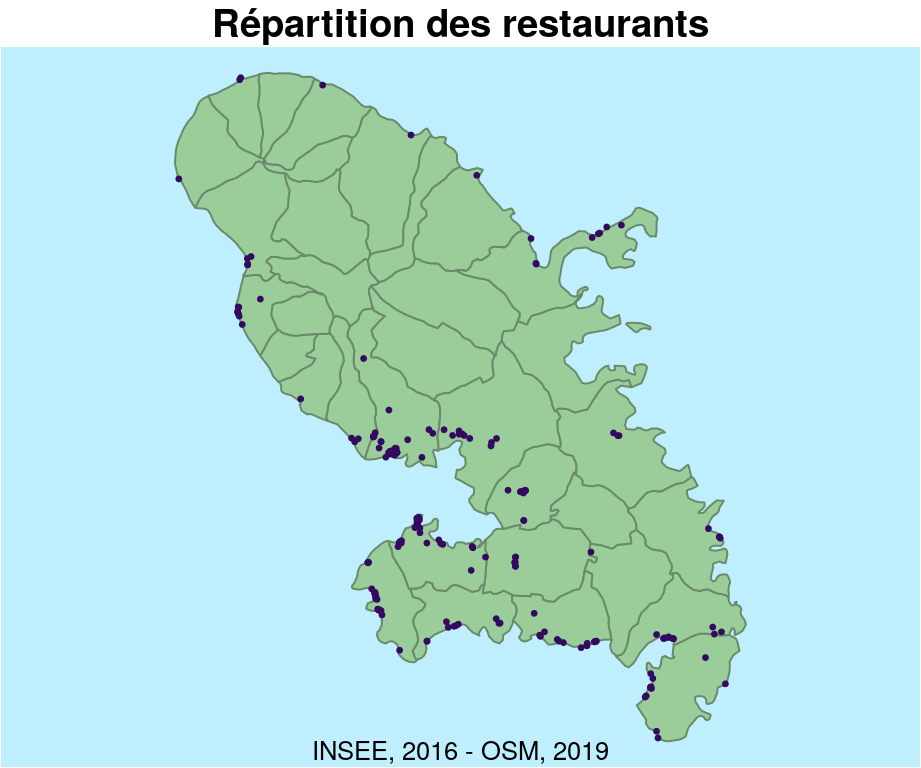
\includegraphics{Cartographie_avec_R_files/figure-latex/unnamed-chunk-14-1} \end{center}

\hypertarget{chapitre2}{\chapter{Cartographie
thématique}\label{chapitre2}}

Nous ne détaillerons pas ici les règles de la cartographie thématique.
Le lecteur pourra se référer à divers ouvrages de référence :
\citet{Bertin67}, \citet{Beguin10}, \citet{Lambert16}

\section{\texorpdfstring{Le package
\texttt{cartography}}{Le package cartography}}\label{le-package-cartography}

Le package \texttt{cartography} \citep{R-cartography} permet de créer et
d'intégrer des cartes thématiques dans sa chaîne de traitements en R. Il
permet des représentations cartographiques telles que les cartes de
symboles proportionnels, des cartes choroplèthes, des typologies, des
cartes de flux ou des cartes de discontinuités. Il offre également des
fonctions qui permettent d'améliorer la réalisation de la carte, comme
des palettes de couleur, des éléments d'habillage (échelle, flèche du
nord, titre, légende\ldots{}), d'y rattacher des labels ou d'accéder à
des APIs cartographiques.

Pour utiliser ce package plusieurs sources peuvent être consultées :

\begin{itemize}
\tightlist
\item
  La documentation du package accessible
  \href{http://riatelab.github.io/cartography/docs/}{sur internet} ou
  directement dans R (\texttt{?cartography}),
\item
  La
  \href{https://CRAN.R-project.org/package=cartography/vignettes/cartography.html}{vignette}
  associée au package présente des exemples de scripts,
\item
  Le blog \href{https://rgeomatic.hypotheses.org/}{R Géomatique} qui met
  à disposition ressources et exemples liés au package et plus
  généralement à l'écosystème spatiale de R,
\item
  La
  \href{http://riatelab.github.io/cartography/vignettes/cheatsheet/cartography_cheatsheet.pdf}{cheat
  sheet} de cartography, qui résume les principales fonctions du package
  de façon synthétique.
\end{itemize}

\begin{center}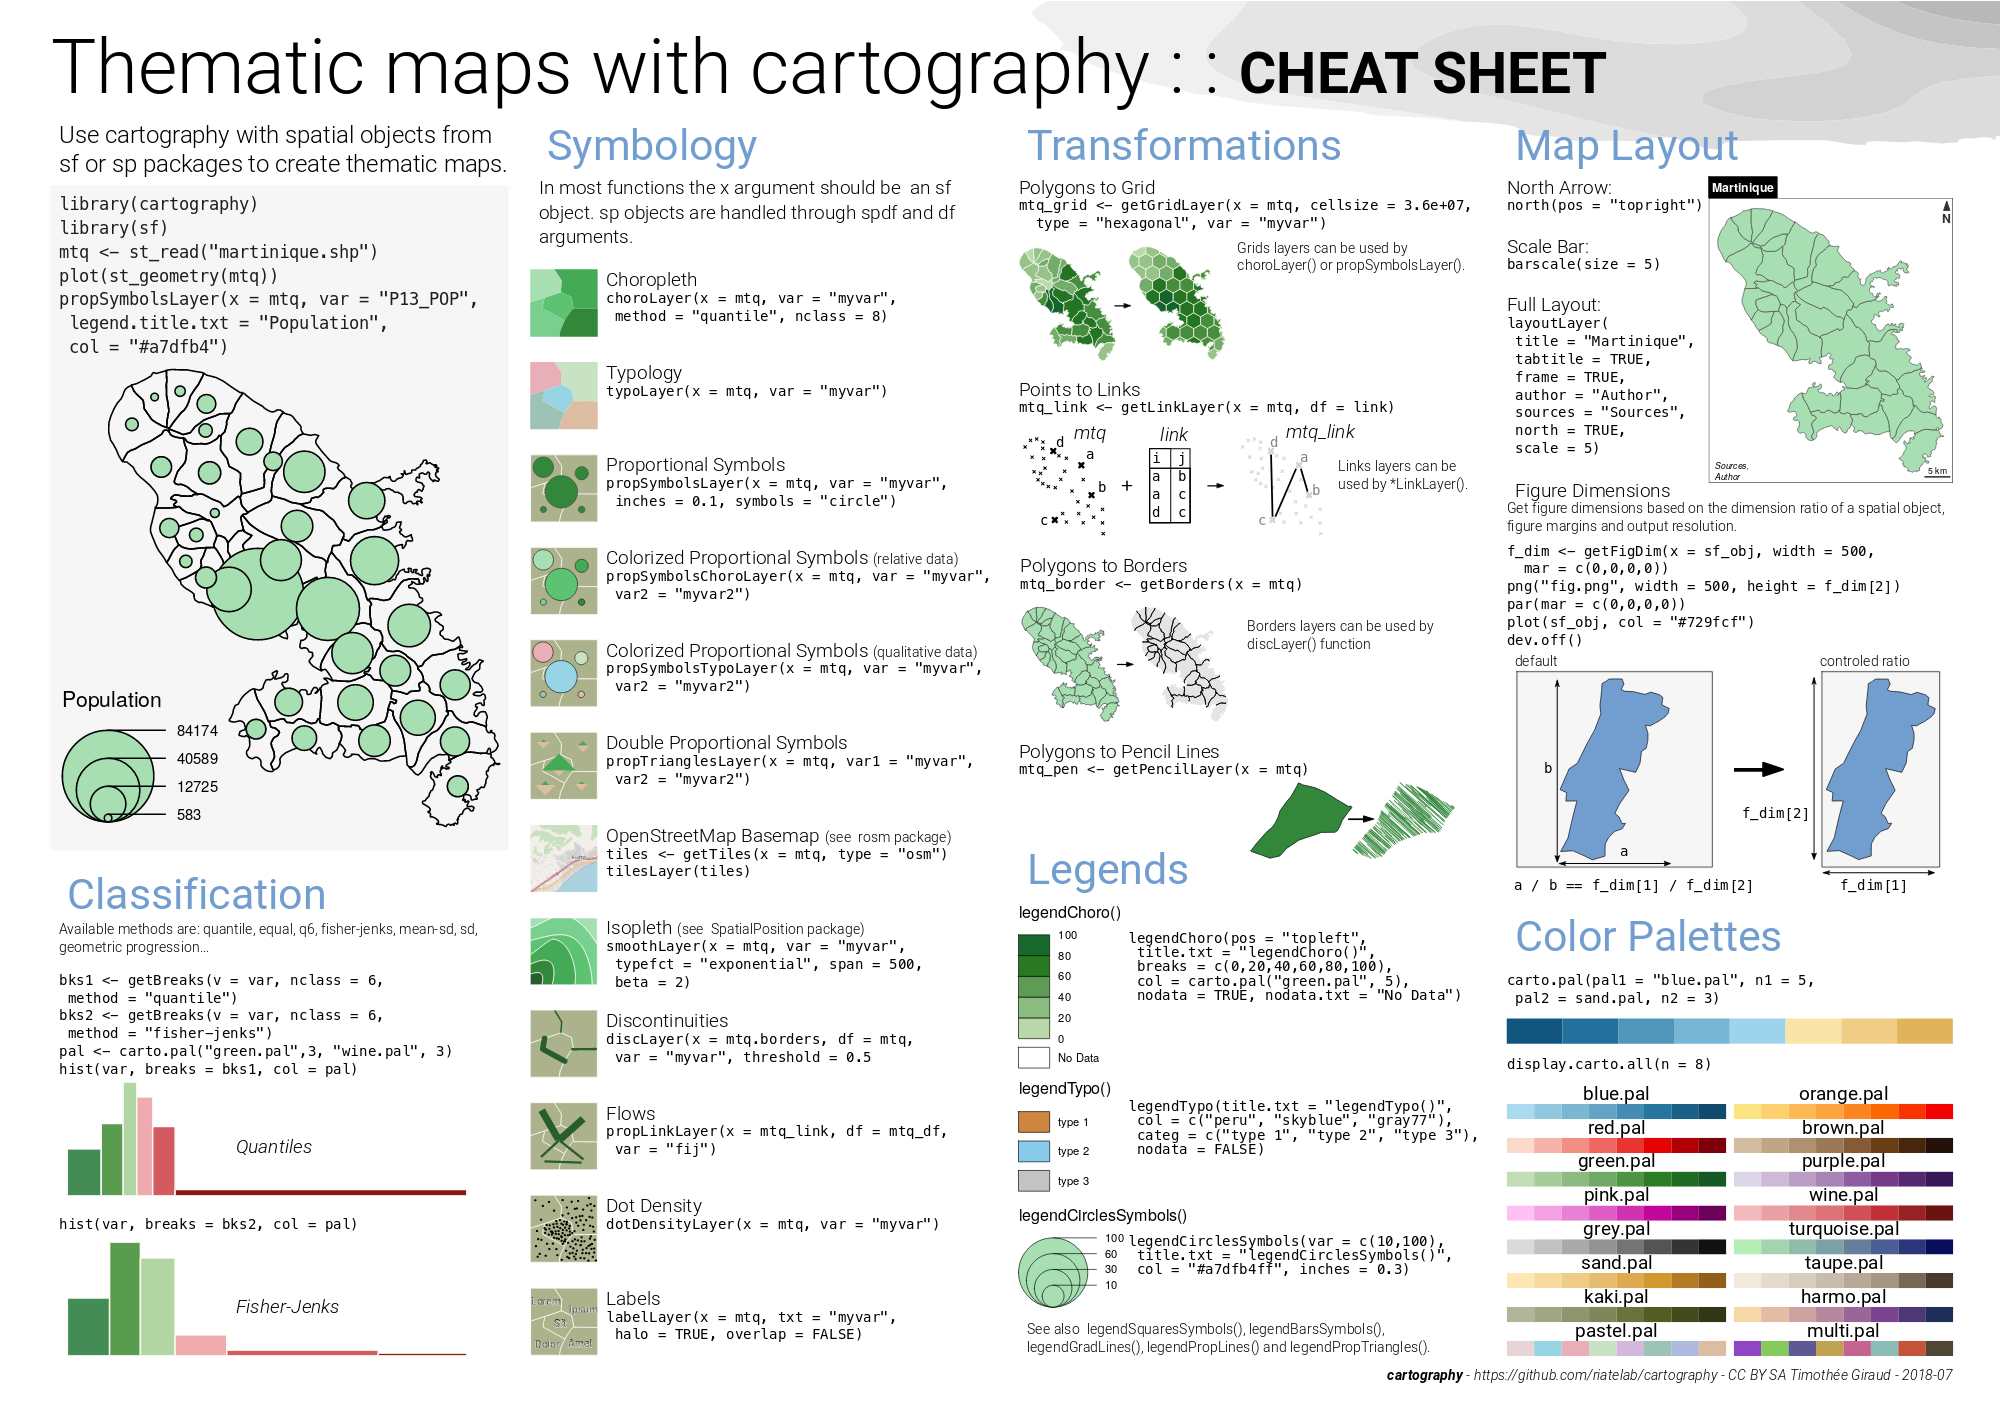
\includegraphics[width=27.78in]{img/cheat_sheet} \end{center}

Les fonctions de \texttt{cartography} dédiées à la représentation
utilisent le suffixe \texttt{Layer}. En général l'argument \texttt{x}
est utilisé par un objet \texttt{sf} et l'argument \texttt{var} sert à
renseigner la variable à représenter.

\section{Représentations usuelles}\label{representations-usuelles}

\subsection{Carte de symboles
proportionnels}\label{carte-de-symboles-proportionnels}

Les cartes de symboles proportionnels sont utilisées pour représenter
les variables de stocks (variables quantitatives absolues, la somme et
la moyenne ont un sens). La fonction \texttt{propSymbolsLayer()} propose
cette représentation, plusieurs symboles sont disponibles : cercles,
carrés et barres.

\begin{Shaded}
\begin{Highlighting}[]
\KeywordTok{library}\NormalTok{(cartography)}
\KeywordTok{library}\NormalTok{(sf)}
\CommentTok{# Import des données}
\NormalTok{mtq <-}\StringTok{ }\KeywordTok{st_read}\NormalTok{(}\StringTok{"data/martinique.shp"}\NormalTok{, }\DataTypeTok{quiet =} \OtherTok{TRUE}\NormalTok{)}
\CommentTok{# Communes}
\KeywordTok{plot}\NormalTok{(}
  \KeywordTok{st_geometry}\NormalTok{(mtq), }
  \DataTypeTok{col =} \StringTok{"lightblue4"}\NormalTok{, }
  \DataTypeTok{border =} \StringTok{"lightblue3"}\NormalTok{, }
  \DataTypeTok{bg =} \StringTok{"lightblue1"}
\NormalTok{)}
\CommentTok{# Symboles proportionnels}
\KeywordTok{propSymbolsLayer}\NormalTok{(}
  \DataTypeTok{x =}\NormalTok{ mtq, }
  \DataTypeTok{var =} \StringTok{"P13_POP"}\NormalTok{, }
  \DataTypeTok{legend.title.txt =} \StringTok{"Population totale}\CharTok{\textbackslash{}n}\StringTok{(2013)"}
\NormalTok{)}
\CommentTok{# Titre}
\KeywordTok{title}\NormalTok{(}\DataTypeTok{main =} \StringTok{"Population en Martinique"}\NormalTok{)}
\end{Highlighting}
\end{Shaded}

\begin{center}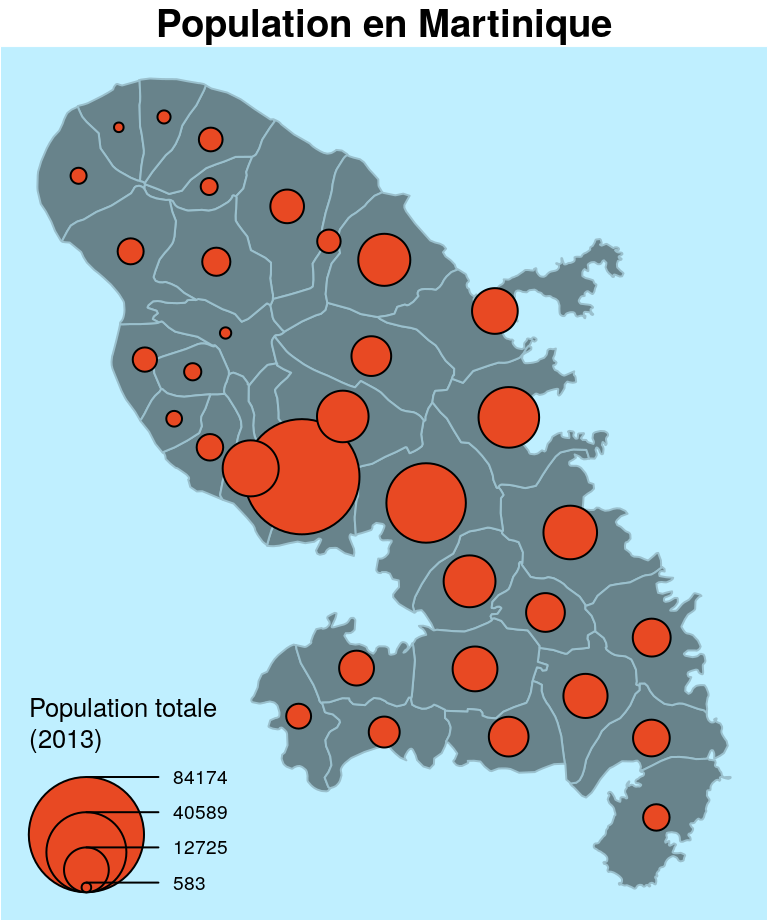
\includegraphics{Cartographie_avec_R_files/figure-latex/propS-1} \end{center}

\subsection{Carte choroplèthe}\label{carte-choroplethe}

Les cartes choroplèthes sont utilisées pour représenter les variables de
ratios (variables quantitatives relatives, la moyenne a un sens, la
somme n'a pas de sens).

Pour ce genre de représentation il faut au préalable :

\begin{itemize}
\tightlist
\item
  choisir une méthode de discrétisation pour transformer une série
  statistique continue en classes définies par des intervalles,
\item
  choisir un nombre de classes,
\item
  choisir une palette de couleurs.
\end{itemize}

La fonction \texttt{choroLayer()} permet de créer des cartes choroplètes
. Les arguments \texttt{nclass}, \texttt{method} et \texttt{breaks}
servent à paramétrer les discrétisations et la fonction
\texttt{getBreaks()} permet de travailler sur les discrétisations en
dehors de la fonction \texttt{choroLayer()}. De même, l'argument
\texttt{col} est utilisé pour renseigner une palette de couleur mais
plusieurs fonctions peuvent être utilisées pour paramétrer les palettes
en dehors de la fonction (\texttt{carto.pal()}\ldots{}).

\begin{Shaded}
\begin{Highlighting}[]
\NormalTok{mtq}\OperatorTok{$}\NormalTok{cagr <-}\StringTok{ }\NormalTok{(((mtq}\OperatorTok{$}\NormalTok{P13_POP }\OperatorTok{/}\StringTok{ }\NormalTok{mtq}\OperatorTok{$}\NormalTok{P08_POP)}\OperatorTok{^}\NormalTok{(}\DecValTok{1}\OperatorTok{/}\DecValTok{4}\NormalTok{)) }\OperatorTok{-}\StringTok{ }\DecValTok{1}\NormalTok{) }\OperatorTok{*}\StringTok{ }\DecValTok{100}
\KeywordTok{choroLayer}\NormalTok{(}
  \DataTypeTok{x =}\NormalTok{ mtq, }
  \DataTypeTok{var =} \StringTok{"cagr"}\NormalTok{, }
  \DataTypeTok{breaks =} \KeywordTok{c}\NormalTok{(}\OperatorTok{-}\FloatTok{6.14}\NormalTok{,}\OperatorTok{-}\DecValTok{2}\NormalTok{,}\OperatorTok{-}\DecValTok{1}\NormalTok{,}\DecValTok{0}\NormalTok{,}\DecValTok{1}\NormalTok{,}\DecValTok{2}\NormalTok{),}
  \DataTypeTok{col =} \KeywordTok{c}\NormalTok{(}\StringTok{"#135D89"}\NormalTok{, }\StringTok{"#4D95BA"}\NormalTok{, }\StringTok{"#96D1EA"}\NormalTok{, }\StringTok{"#FCDACA"}\NormalTok{, }\StringTok{"#EC4E49"}\NormalTok{),}
  \DataTypeTok{legend.title.txt =} \StringTok{"Taux de croissance}\CharTok{\textbackslash{}n}\StringTok{annuel moyen}\CharTok{\textbackslash{}n}\StringTok{(2008-2013)"}
\NormalTok{)}
\KeywordTok{title}\NormalTok{(}\DataTypeTok{main =} \StringTok{"Evolution de la population"}\NormalTok{)}
\end{Highlighting}
\end{Shaded}

\begin{center}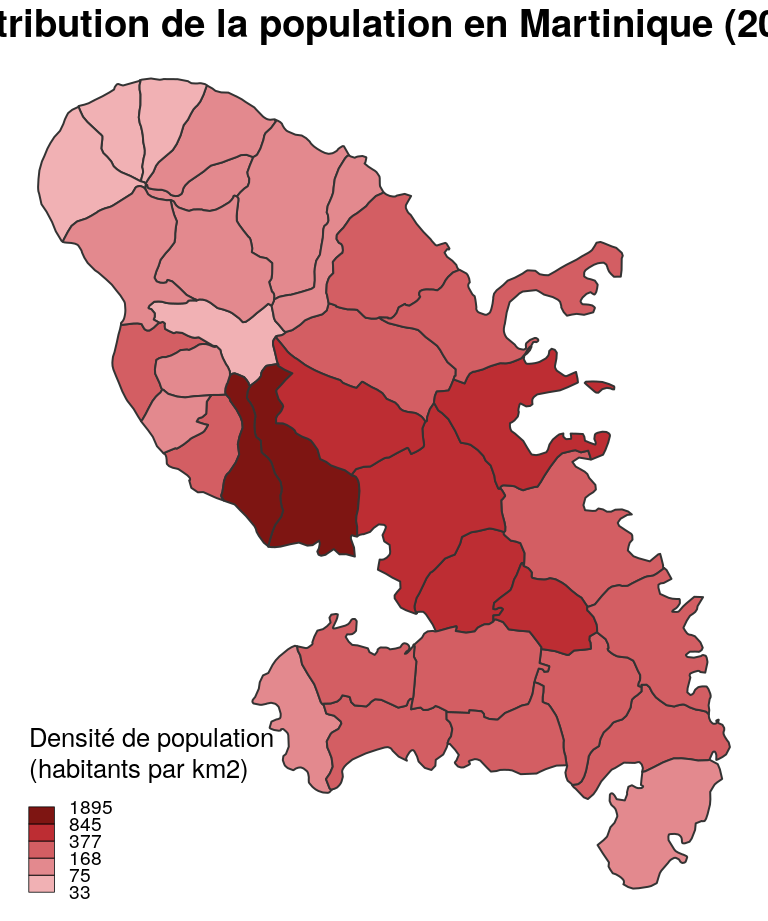
\includegraphics{Cartographie_avec_R_files/figure-latex/choro-1} \end{center}

\subsubsection{Discrétisations}\label{discretisation}

La fonction \texttt{getBreaks()} met à disposition les méthodes de
discrétisations de variables classique : quantiles, moyenn/écart-type,
amplitudes égales, moyennes emboitées, Fisher-Jenks, géométrique
\ldots{}

\begin{Shaded}
\begin{Highlighting}[]
\NormalTok{var <-}\StringTok{ }\NormalTok{mtq}\OperatorTok{$}\NormalTok{cagr}
\NormalTok{moy <-}\StringTok{ }\KeywordTok{mean}\NormalTok{(var)}
\NormalTok{med <-}\StringTok{ }\KeywordTok{median}\NormalTok{(var)}
\NormalTok{std <-}\StringTok{ }\KeywordTok{sd}\NormalTok{(var)}
\CommentTok{# Quantile intervals}
\NormalTok{breaks <-}\StringTok{ }\KeywordTok{getBreaks}\NormalTok{(}\DataTypeTok{v =}\NormalTok{ var, }\DataTypeTok{nclass =} \DecValTok{6}\NormalTok{, }\DataTypeTok{method =} \StringTok{"quantile"}\NormalTok{)}
\KeywordTok{hist}\NormalTok{(var, }\DataTypeTok{probability =} \OtherTok{TRUE}\NormalTok{, }\DataTypeTok{breaks =}\NormalTok{ breaks, }\DataTypeTok{main=}\StringTok{"quantiles"}\NormalTok{,}
     \DataTypeTok{col =} \KeywordTok{carto.pal}\NormalTok{(}\DataTypeTok{pal1 =} \StringTok{"wine.pal"}\NormalTok{,}\DecValTok{3}\NormalTok{, }\StringTok{"green.pal"}\NormalTok{, }\DecValTok{3}\NormalTok{))}
\KeywordTok{rug}\NormalTok{(var)}
\KeywordTok{abline}\NormalTok{(}\DataTypeTok{v =}\NormalTok{ med, }\DataTypeTok{col =} \StringTok{"blue"}\NormalTok{, }\DataTypeTok{lwd =} \DecValTok{3}\NormalTok{)}
\end{Highlighting}
\end{Shaded}

\begin{center}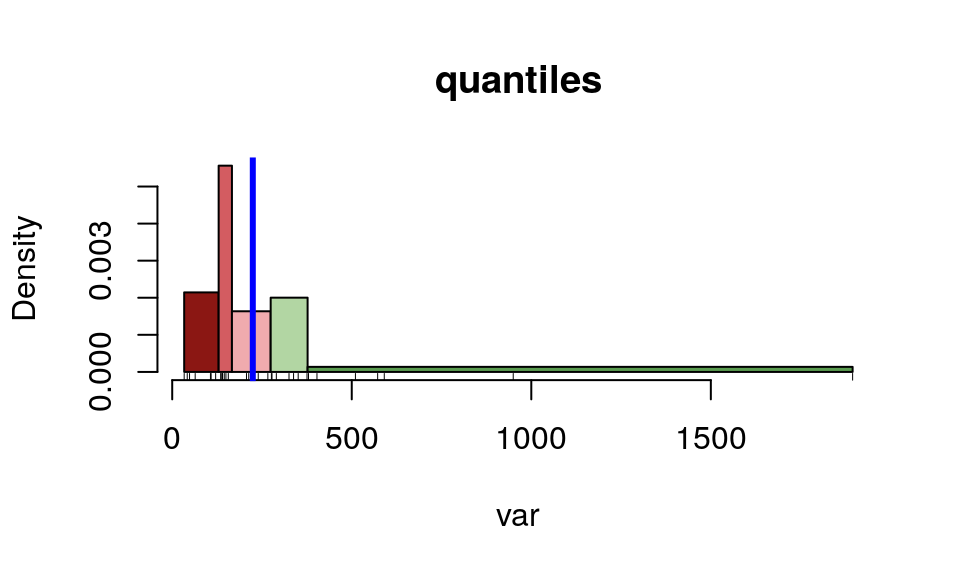
\includegraphics{Cartographie_avec_R_files/figure-latex/discr2-1} \end{center}

\begin{Shaded}
\begin{Highlighting}[]
\CommentTok{# Mean and standard deviation (msd)}
\NormalTok{breaks <-}\StringTok{ }\KeywordTok{getBreaks}\NormalTok{(}\DataTypeTok{v =}\NormalTok{ var, }\DataTypeTok{method =} \StringTok{"msd"}\NormalTok{, }\DataTypeTok{k =} \DecValTok{1}\NormalTok{, }\DataTypeTok{middle =} \OtherTok{TRUE}\NormalTok{)}
\KeywordTok{hist}\NormalTok{(var, }\DataTypeTok{probability =} \OtherTok{TRUE}\NormalTok{, }\DataTypeTok{breaks =}\NormalTok{ breaks, }\DataTypeTok{main=}\StringTok{"moyenne / écart-type"}\NormalTok{,}
     \DataTypeTok{col =} \KeywordTok{carto.pal}\NormalTok{(}\DataTypeTok{pal1 =} \StringTok{"wine.pal"}\NormalTok{,}\DecValTok{3}\NormalTok{ , }\StringTok{"green.pal"}\NormalTok{, }\DecValTok{2}\NormalTok{, }\DataTypeTok{middle =} \OtherTok{TRUE}\NormalTok{))}
\KeywordTok{rug}\NormalTok{(var)}
\KeywordTok{abline}\NormalTok{(}\DataTypeTok{v =}\NormalTok{ moy, }\DataTypeTok{col =} \StringTok{"red"}\NormalTok{, }\DataTypeTok{lwd =} \DecValTok{3}\NormalTok{)}
\KeywordTok{abline}\NormalTok{(}\DataTypeTok{v =}\NormalTok{ moy }\OperatorTok{+}\StringTok{ }\FloatTok{0.5} \OperatorTok{*}\StringTok{ }\NormalTok{std, }\DataTypeTok{col =} \StringTok{"blue"}\NormalTok{, }\DataTypeTok{lwd =} \DecValTok{3}\NormalTok{)}
\KeywordTok{abline}\NormalTok{(}\DataTypeTok{v =}\NormalTok{ moy }\OperatorTok{-}\StringTok{ }\FloatTok{0.5} \OperatorTok{*}\StringTok{ }\NormalTok{std, }\DataTypeTok{col =} \StringTok{"blue"}\NormalTok{, }\DataTypeTok{lwd =} \DecValTok{3}\NormalTok{)}
\end{Highlighting}
\end{Shaded}

\begin{center}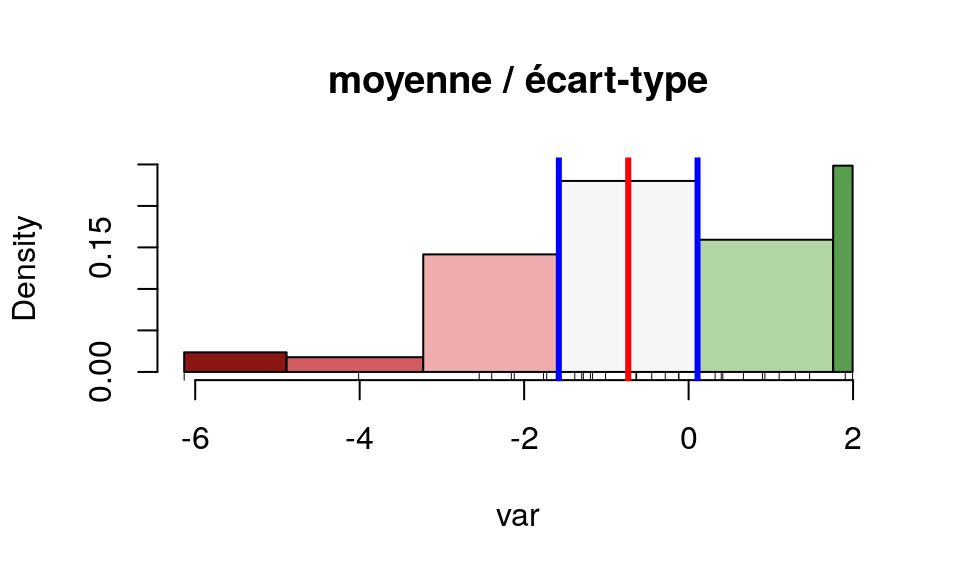
\includegraphics{Cartographie_avec_R_files/figure-latex/discr3-1} \end{center}

\subsubsection{Palettes de couleurs}\label{palettes}

La fonction \texttt{display.carto.all()} permet d'afficher toutes
palettes de couleurs disponibles dans \texttt{cartography}.

\begin{Shaded}
\begin{Highlighting}[]
\KeywordTok{display.carto.all}\NormalTok{(}\DecValTok{20}\NormalTok{)}
\end{Highlighting}
\end{Shaded}

\begin{center}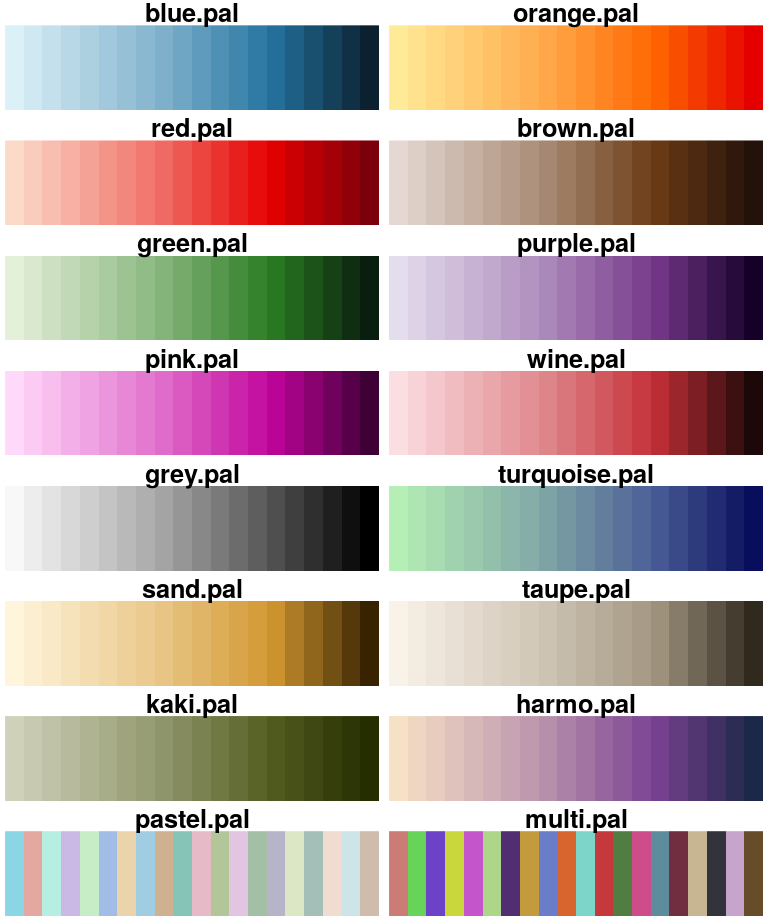
\includegraphics{Cartographie_avec_R_files/figure-latex/pa-1} \end{center}

La fonction \texttt{display.carto.pal()} permet de détailler une palette
de couleurs.

\begin{Shaded}
\begin{Highlighting}[]
\KeywordTok{display.carto.pal}\NormalTok{(}\StringTok{"turquoise.pal"}\NormalTok{)}
\end{Highlighting}
\end{Shaded}

\begin{center}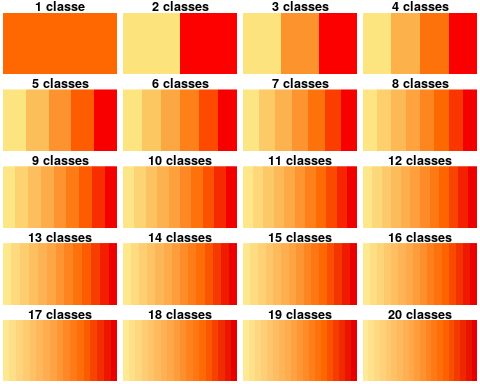
\includegraphics{Cartographie_avec_R_files/figure-latex/pal1-1} \end{center}

La fonction \texttt{carto.pal()} permet de construire une palette de
couleur. Il est possible de créer des palettes associant 2 couleurs.

\begin{Shaded}
\begin{Highlighting}[]
\NormalTok{mypal <-}\StringTok{ }\KeywordTok{carto.pal}\NormalTok{(}\DataTypeTok{pal1 =} \StringTok{"wine.pal"}\NormalTok{, }\DataTypeTok{n1 =} \DecValTok{5}\NormalTok{, }\DataTypeTok{pal2 =} \StringTok{"green.pal"}\NormalTok{, }\DataTypeTok{n2 =} \DecValTok{4}\NormalTok{)}
\KeywordTok{image}\NormalTok{(}\DecValTok{1}\OperatorTok{:}\DecValTok{9}\NormalTok{, }\DecValTok{1}\NormalTok{, }\KeywordTok{as.matrix}\NormalTok{(}\DecValTok{1}\OperatorTok{:}\DecValTok{9}\NormalTok{), }\DataTypeTok{col=}\NormalTok{mypal, }\DataTypeTok{xlab =} \StringTok{""}\NormalTok{, }\DataTypeTok{ylab =} \StringTok{""}\NormalTok{, }\DataTypeTok{xaxt =} \StringTok{"n"}\NormalTok{, }
      \DataTypeTok{yaxt =} \StringTok{"n"}\NormalTok{,}\DataTypeTok{bty =} \StringTok{"n"}\NormalTok{)}
\end{Highlighting}
\end{Shaded}

\begin{center}
\includegraphics{Cartographie_avec_R_files/figure-latex/pal2-1} \end{center}

\subsection{Carte de typologie}\label{carte-de-typologie}

Les cartes de typologies sont utilisées pour représenter les variables
qualitatives. La fonction \texttt{typoLayer()} propose cette
représentation. L'argument \texttt{legend.values.order} sert à ordonner
les modalités dans la légende.

\begin{Shaded}
\begin{Highlighting}[]
\KeywordTok{typoLayer}\NormalTok{(}
  \DataTypeTok{x =}\NormalTok{ mtq, }
  \DataTypeTok{var=}\StringTok{"STATUT"}\NormalTok{,}
  \DataTypeTok{legend.values.order =} \KeywordTok{c}\NormalTok{(}\StringTok{"Préfecture de région"}\NormalTok{,}
                          \StringTok{"Sous-préfecture"}\NormalTok{, }
                          \StringTok{"Commune simple"}\NormalTok{),}
  \DataTypeTok{col =} \KeywordTok{c}\NormalTok{(}\StringTok{"aquamarine4"}\NormalTok{, }\StringTok{"yellow3"}\NormalTok{,}\StringTok{"wheat"}\NormalTok{),}
  \DataTypeTok{legend.pos =} \StringTok{"topright"}\NormalTok{,}
  \DataTypeTok{legend.title.txt =} \StringTok{"Statut administratif"}
\NormalTok{)}
\KeywordTok{title}\NormalTok{(}\StringTok{"Statut Administratif"}\NormalTok{)}
\end{Highlighting}
\end{Shaded}

\begin{center}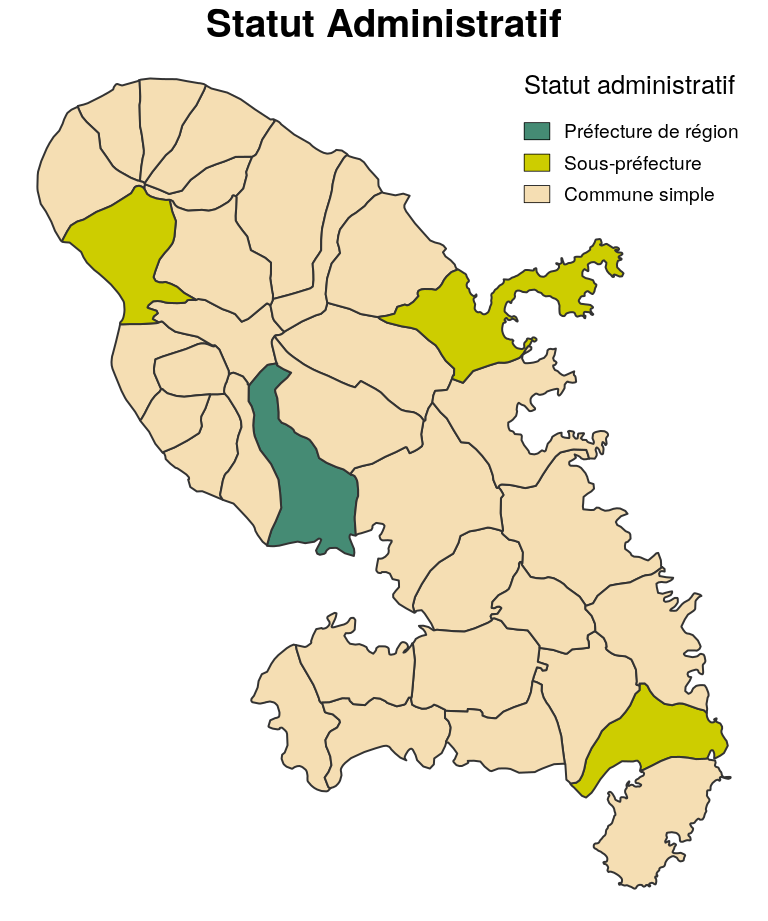
\includegraphics{Cartographie_avec_R_files/figure-latex/typolo-1} \end{center}

\section{Combinaisons de
représentations}\label{combinaisons-de-representations}

Plusieurs fonctions sont dédiées à la représentation combinée de 2
variables.

\subsection{Carte de stocks et de
ratios}\label{carte-de-stocks-et-de-ratios}

La fonction \texttt{propSymbolsChoroLayer()} représente des symboles
proportionnels dont les surfaces sont proportionnelles aux valeurs d'une
variable et dont la couleur repose sur la discrétisation d'une seconde
variable. La fonction utilise les arguments des fonctions
\texttt{propSymbolsLayer()} et \texttt{choroLayer()}.

\begin{Shaded}
\begin{Highlighting}[]
\KeywordTok{plot}\NormalTok{(}
  \KeywordTok{st_geometry}\NormalTok{(mtq), }
  \DataTypeTok{col=}\StringTok{"darkseagreen3"}\NormalTok{, }
  \DataTypeTok{border=}\StringTok{"darkseagreen4"}\NormalTok{,  }
  \DataTypeTok{bg =} \StringTok{"lightblue1"}
\NormalTok{)}
\KeywordTok{propSymbolsChoroLayer}\NormalTok{(}
  \DataTypeTok{x =}\NormalTok{ mtq, }
  \DataTypeTok{var=} \StringTok{"P13_POP"}\NormalTok{,}
  \DataTypeTok{var2 =} \StringTok{"cagr"}\NormalTok{, }
  \DataTypeTok{breaks =} \KeywordTok{c}\NormalTok{(}\OperatorTok{-}\FloatTok{6.14}\NormalTok{,}\OperatorTok{-}\DecValTok{2}\NormalTok{,}\OperatorTok{-}\DecValTok{1}\NormalTok{,}\DecValTok{0}\NormalTok{,}\DecValTok{1}\NormalTok{,}\DecValTok{2}\NormalTok{),}
  \DataTypeTok{col =} \KeywordTok{c}\NormalTok{(}\StringTok{"#135D89"}\NormalTok{, }\StringTok{"#4D95BA"}\NormalTok{, }\StringTok{"#96D1EA"}\NormalTok{, }\StringTok{"#FCDACA"}\NormalTok{, }\StringTok{"#EC4E49"}\NormalTok{),}
  \DataTypeTok{legend.var.pos =} \StringTok{"topright"}\NormalTok{,}
  \DataTypeTok{legend.var.title.txt =} \StringTok{"Population totale}\CharTok{\textbackslash{}n}\StringTok{(2013)"}\NormalTok{,}
  \DataTypeTok{legend.var2.pos =} \StringTok{"bottomleft"}\NormalTok{,}
  \DataTypeTok{legend.var2.title.txt =} \StringTok{"Taux de croissance}\CharTok{\textbackslash{}n}\StringTok{annuel moyen}\CharTok{\textbackslash{}n}\StringTok{(2008-2013)"}
\NormalTok{)}
\KeywordTok{title}\NormalTok{(}\StringTok{"Evolution de la population"}\NormalTok{)}
\end{Highlighting}
\end{Shaded}

\begin{center}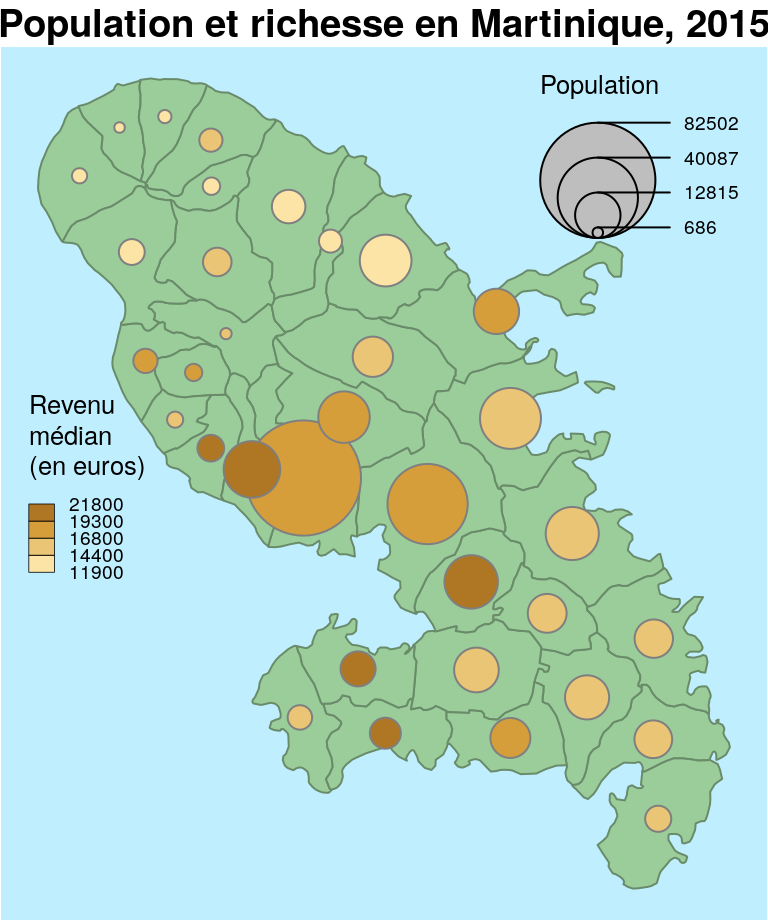
\includegraphics{Cartographie_avec_R_files/figure-latex/choroprop-1} \end{center}

\subsection{Carte de stocks et de
qualitative}\label{carte-de-stocks-et-de-qualitative}

La fonction \texttt{propSymbolsTypoLayer()} représente des symboles
proportionnels dont les surfaces sont proportionnelles aux valeurs d'une
variable et dont la couleur représente les modalités d'une variable
qualitative. La fonction utilise les arguments des fonctions
\texttt{propSymbolsLayer()} et \texttt{typoLayer()}.

\begin{Shaded}
\begin{Highlighting}[]
\KeywordTok{plot}\NormalTok{(}
  \KeywordTok{st_geometry}\NormalTok{(mtq), }
  \DataTypeTok{col=}\StringTok{"darkseagreen3"}\NormalTok{, }
  \DataTypeTok{border=}\StringTok{"darkseagreen4"}\NormalTok{,  }
  \DataTypeTok{bg =} \StringTok{"lightblue1"}
\NormalTok{)}
\KeywordTok{propSymbolsTypoLayer}\NormalTok{(}
  \DataTypeTok{x =}\NormalTok{ mtq, }
  \DataTypeTok{var =} \StringTok{"P13_POP"}\NormalTok{, }
  \DataTypeTok{symbols =} \StringTok{"circle"}\NormalTok{,}
  \DataTypeTok{var2 =} \StringTok{"STATUT"}\NormalTok{,}
  \DataTypeTok{col =} \KeywordTok{c}\NormalTok{(}\StringTok{"aquamarine4"}\NormalTok{, }\StringTok{"yellow3"}\NormalTok{,}\StringTok{"wheat"}\NormalTok{),}
  \DataTypeTok{legend.var.pos =} \StringTok{"bottomleft"}\NormalTok{,}
  \DataTypeTok{legend.var.title.txt =} \StringTok{"Population totale}\CharTok{\textbackslash{}n}\StringTok{(2013)"}\NormalTok{,}
  \DataTypeTok{legend.var2.title.txt =} \StringTok{"Statut administratif"}\NormalTok{,}
  \DataTypeTok{legend.var2.values.order =} \KeywordTok{c}\NormalTok{(}\StringTok{"Préfecture de région"}\NormalTok{,}
                               \StringTok{"Sous-préfecture"}\NormalTok{,}
                               \StringTok{"Commune simple"}\NormalTok{)}
\NormalTok{)}
\KeywordTok{title}\NormalTok{(}\StringTok{"Population en Martinique"}\NormalTok{)}
\end{Highlighting}
\end{Shaded}

\begin{center}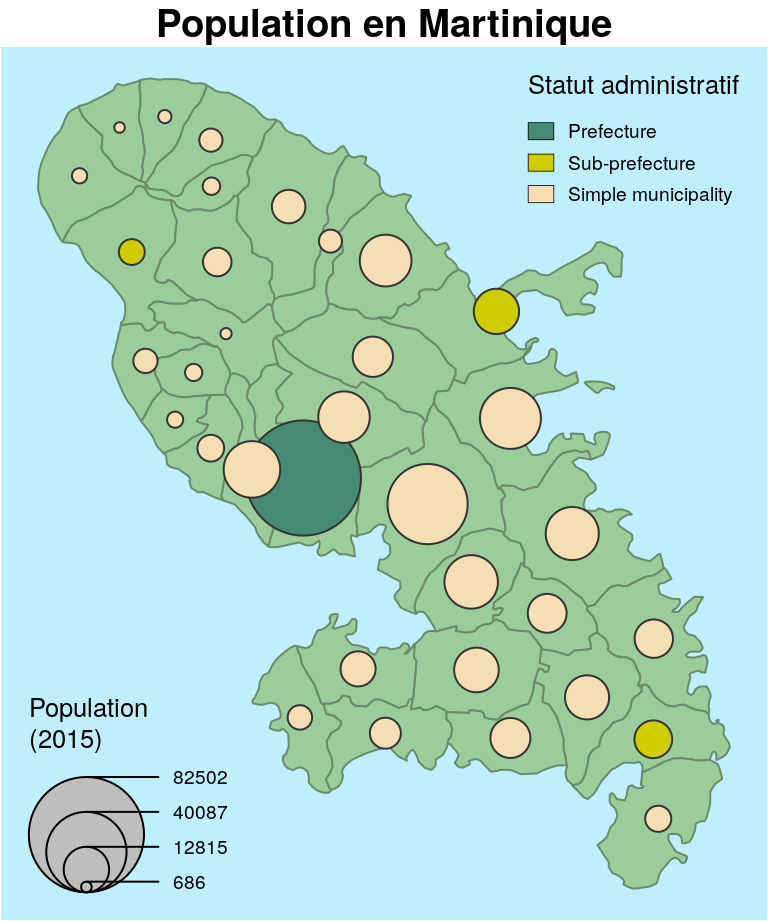
\includegraphics{Cartographie_avec_R_files/figure-latex/typoprop-1} \end{center}

\section{Éléments d'habillage}\label{elements-dhabillage}

Pour être finalisée, une carte thématique doit contenir certains
éléments aditionnels tels que : le titre, l'auteur, la source,
l'échelle, l'orientation\ldots{}

\subsection{Habillage complet}\label{habillage-complet}

La fonction \texttt{layoutLayer()} permet d'afficher tous ces éléments.

\begin{Shaded}
\begin{Highlighting}[]
\KeywordTok{plot}\NormalTok{(}\KeywordTok{st_geometry}\NormalTok{(mtq), }\DataTypeTok{col =} \StringTok{"lightblue4"}\NormalTok{, }\DataTypeTok{border =} \StringTok{"lightblue3"}\NormalTok{, }
     \DataTypeTok{bg =} \StringTok{"lightblue1"}\NormalTok{)}
\KeywordTok{layoutLayer}\NormalTok{(}
  \DataTypeTok{title =} \StringTok{"Martinique"}\NormalTok{, }
  \DataTypeTok{sources =} \StringTok{"IGN"}\NormalTok{, }
  \DataTypeTok{author =} \StringTok{"Giraud & Pécout, 2019"}\NormalTok{,}
  \DataTypeTok{north =} \OtherTok{TRUE}
\NormalTok{)}
\end{Highlighting}
\end{Shaded}

\begin{center}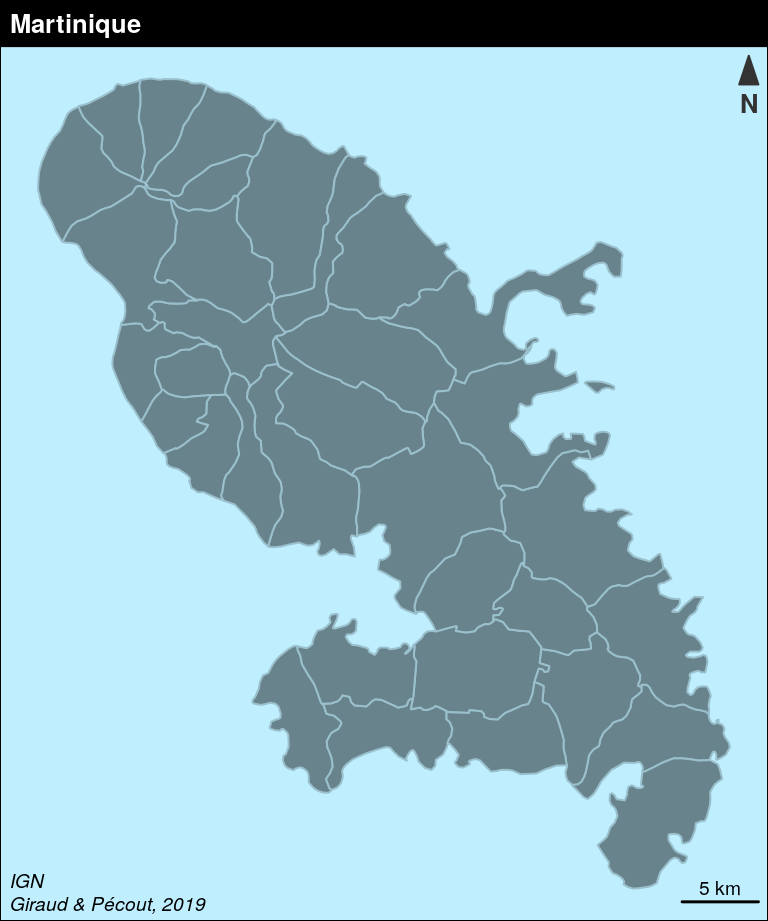
\includegraphics{Cartographie_avec_R_files/figure-latex/layout1-1} \end{center}

Plusieurs arguments permettent de paramétrer plus finement les éléments
d'habillage pour aboutir à des cartes plus personnalisées
(\texttt{tabtitle}, \texttt{col}, \texttt{coltitle},
\texttt{theme}\ldots{}).

\begin{Shaded}
\begin{Highlighting}[]
\KeywordTok{plot}\NormalTok{(}\KeywordTok{st_geometry}\NormalTok{(mtq), }\DataTypeTok{col =} \StringTok{"lightblue4"}\NormalTok{, }\DataTypeTok{border =} \StringTok{"lightblue3"}\NormalTok{, }
     \DataTypeTok{bg =} \StringTok{"lightblue1"}\NormalTok{)}
\KeywordTok{layoutLayer}\NormalTok{(}
  \DataTypeTok{title =} \StringTok{"Martinique"}\NormalTok{, }
  \DataTypeTok{sources =} \StringTok{"IGN"}\NormalTok{, }
  \DataTypeTok{author =} \StringTok{"Giraud & Pécout, 2019"}\NormalTok{,}
  \DataTypeTok{north =} \OtherTok{TRUE}\NormalTok{, }
  \DataTypeTok{scale =} \DecValTok{5}\NormalTok{,}
  \DataTypeTok{frame =} \OtherTok{FALSE}\NormalTok{, }
  \DataTypeTok{tabtitle =} \OtherTok{TRUE}\NormalTok{, }
  \DataTypeTok{theme =} \StringTok{"turquoise.pal"}
\NormalTok{)}
\end{Highlighting}
\end{Shaded}

\begin{center}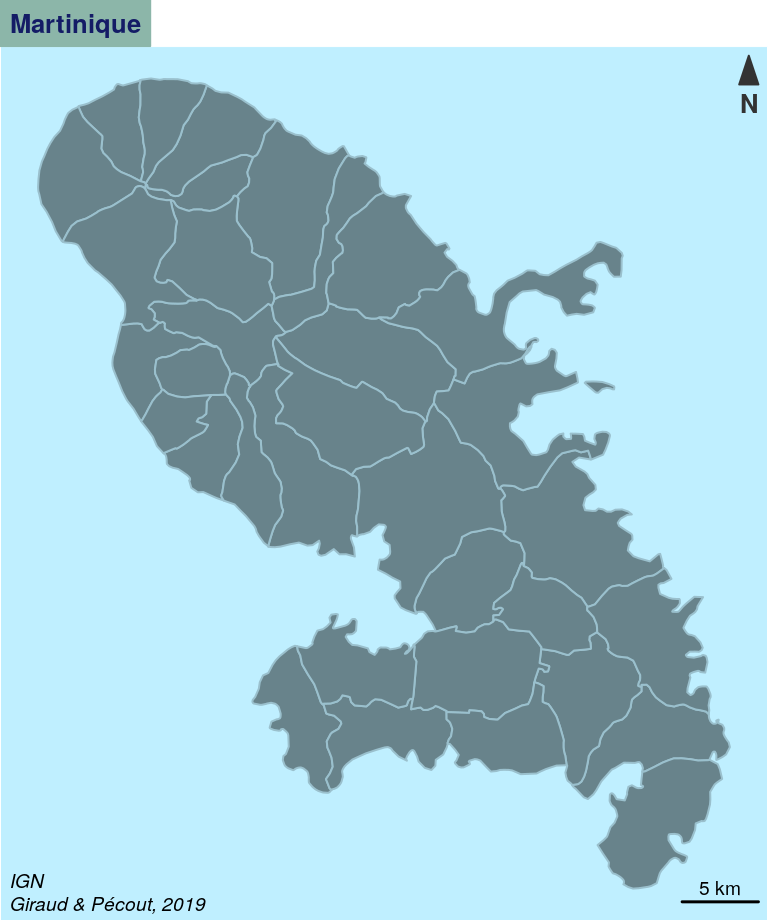
\includegraphics{Cartographie_avec_R_files/figure-latex/layout2-1} \end{center}

\subsection{Flèche d'orientation}\label{fleche-dorientation}

La fonction \texttt{north()} permet de mieux choisir la position et
l'aspect de la flêche d'orientation.

\begin{Shaded}
\begin{Highlighting}[]
\KeywordTok{plot}\NormalTok{(}\KeywordTok{st_geometry}\NormalTok{(mtq), }\DataTypeTok{col =} \StringTok{"#D1914D"}\NormalTok{, }\DataTypeTok{border =} \StringTok{"white"}\NormalTok{)}
\KeywordTok{north}\NormalTok{(}\DataTypeTok{pos =} \StringTok{"topleft"}\NormalTok{, }\DataTypeTok{col =} \StringTok{"#D1914D"}\NormalTok{)}
\KeywordTok{layoutLayer}\NormalTok{(}\DataTypeTok{title =} \StringTok{"Martinique"}\NormalTok{, }\DataTypeTok{sources =} \StringTok{"IGN"}\NormalTok{, }
            \DataTypeTok{author =} \StringTok{"Giraud & Pécout, 2019"}\NormalTok{, }\DataTypeTok{frame =} \OtherTok{FALSE}\NormalTok{, }\DataTypeTok{scale =} \DecValTok{5}\NormalTok{,}
            \DataTypeTok{coltitle =} \StringTok{"#D1914D"}\NormalTok{,}\DataTypeTok{tabtitle =} \OtherTok{TRUE}\NormalTok{, }\DataTypeTok{postitle =} \StringTok{"right"}\NormalTok{)}
\end{Highlighting}
\end{Shaded}

\begin{center}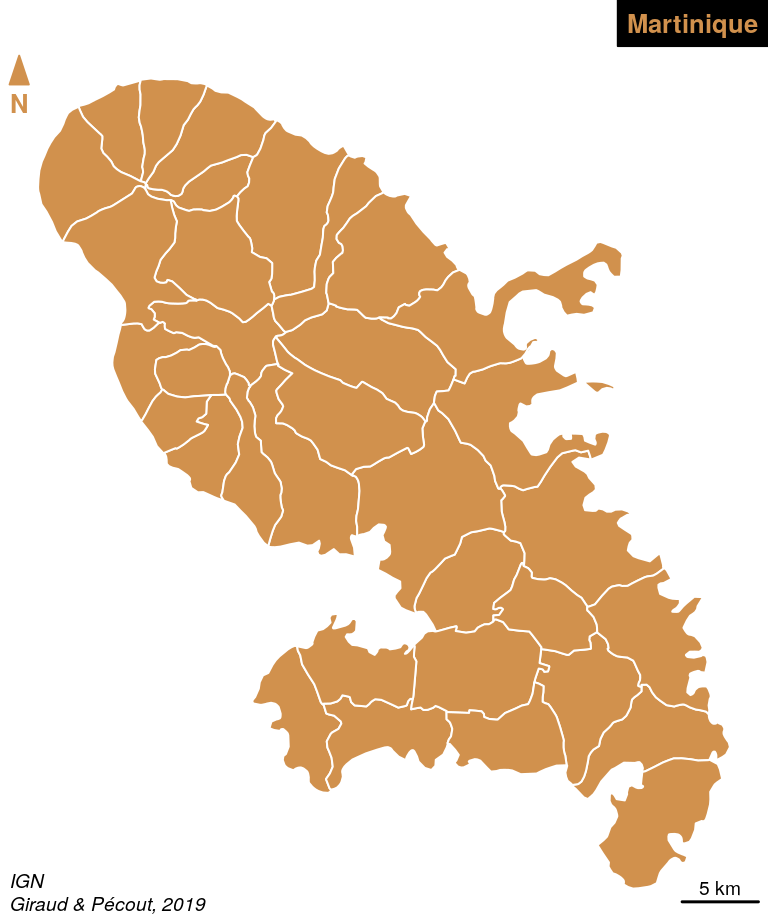
\includegraphics{Cartographie_avec_R_files/figure-latex/north-1} \end{center}

\subsection{Échelle}\label{echelle}

La fonction \texttt{barscale()} permet de mieux choisir la position et
l'aspect de l'échelle.

\begin{Shaded}
\begin{Highlighting}[]
\KeywordTok{plot}\NormalTok{(}\KeywordTok{st_geometry}\NormalTok{(mtq), }\DataTypeTok{col =} \StringTok{"#D1914D"}\NormalTok{, }\DataTypeTok{border =} \StringTok{"white"}\NormalTok{)}
\KeywordTok{barscale}\NormalTok{(}
  \DataTypeTok{size =} \DecValTok{5}\NormalTok{, }
  \DataTypeTok{lwd =} \DecValTok{2}\NormalTok{, }
  \DataTypeTok{cex =} \FloatTok{1.2}\NormalTok{, }
  \DataTypeTok{pos =} \KeywordTok{c}\NormalTok{(}\FloatTok{713712.6}\NormalTok{,}\DecValTok{1594777}\NormalTok{)}
\NormalTok{)}
\KeywordTok{layoutLayer}\NormalTok{(}\DataTypeTok{title =} \StringTok{"Martinique"}\NormalTok{, }\DataTypeTok{sources =} \StringTok{"IGN"}\NormalTok{, }
            \DataTypeTok{author =} \StringTok{"Giraud & Pécout, 2019"}\NormalTok{, }\DataTypeTok{frame =} \OtherTok{FALSE}\NormalTok{, }\DataTypeTok{scale =} \OtherTok{NULL}\NormalTok{,}
            \DataTypeTok{coltitle =} \StringTok{"#D1914D"}\NormalTok{,}\DataTypeTok{tabtitle =} \OtherTok{TRUE}\NormalTok{)}
\end{Highlighting}
\end{Shaded}

\begin{center}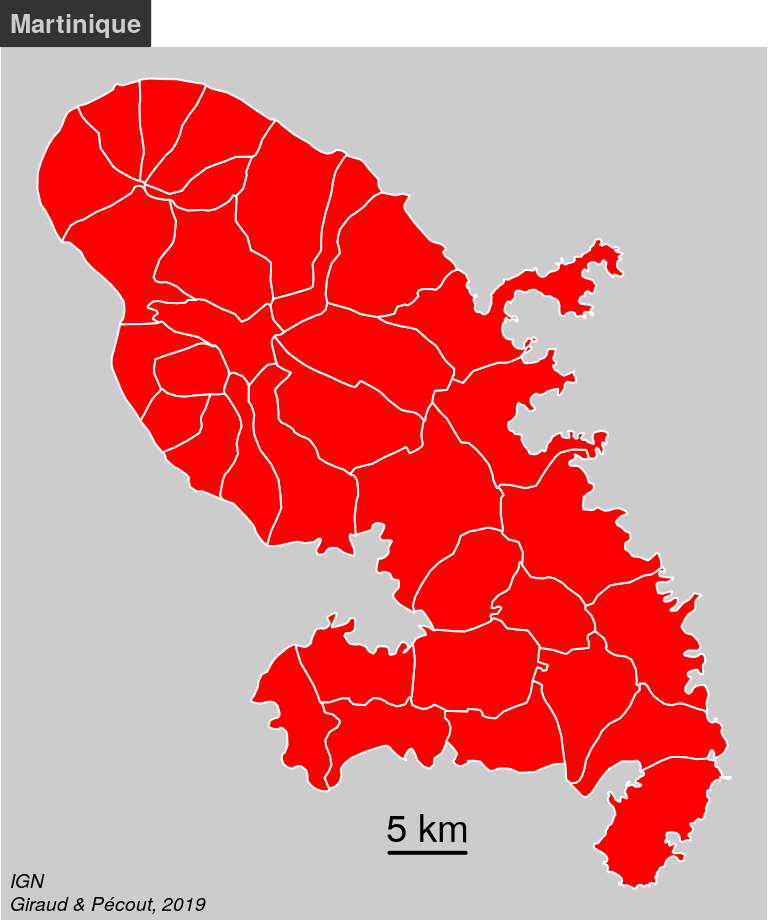
\includegraphics{Cartographie_avec_R_files/figure-latex/scale-1} \end{center}

\subsection{Étiquettes}\label{etiquettes}

La fonction \texttt{labelLayer()} est dédiée à l'afichage d'étiquettes.

\begin{Shaded}
\begin{Highlighting}[]
\KeywordTok{plot}\NormalTok{(}\KeywordTok{st_geometry}\NormalTok{(mtq), }\DataTypeTok{col =} \StringTok{"darkseagreen3"}\NormalTok{, }\DataTypeTok{border =} \StringTok{"darkseagreen4"}\NormalTok{, }
     \DataTypeTok{bg =} \StringTok{"#A6CAE0"}\NormalTok{)}
\KeywordTok{labelLayer}\NormalTok{(}
  \DataTypeTok{x =}\NormalTok{ mtq, }
  \DataTypeTok{txt =} \StringTok{"LIBGEO"}\NormalTok{, }
  \DataTypeTok{col=} \StringTok{"black"}\NormalTok{, }
  \DataTypeTok{cex =} \FloatTok{0.7}\NormalTok{, }
  \DataTypeTok{font =} \DecValTok{4}\NormalTok{,}
  \DataTypeTok{halo =} \OtherTok{TRUE}\NormalTok{, }
  \DataTypeTok{bg =} \StringTok{"white"}\NormalTok{, }
  \DataTypeTok{r =} \FloatTok{0.1}\NormalTok{, }
  \DataTypeTok{overlap =} \OtherTok{FALSE}\NormalTok{, }
  \DataTypeTok{show.lines =} \OtherTok{FALSE}
\NormalTok{)}
\KeywordTok{layoutLayer}\NormalTok{(}\DataTypeTok{title =} \StringTok{"Communes"}\NormalTok{, }\DataTypeTok{tabtitle =} \OtherTok{TRUE}\NormalTok{, }\DataTypeTok{author =} \StringTok{"INSEE, 2016"}\NormalTok{, }
            \DataTypeTok{sources =}\StringTok{""}\NormalTok{, }\DataTypeTok{north =}\OtherTok{TRUE}\NormalTok{, }\DataTypeTok{frame =} \OtherTok{FALSE}\NormalTok{, }\DataTypeTok{scale =} \DecValTok{5}\NormalTok{)}
\end{Highlighting}
\end{Shaded}

\begin{center}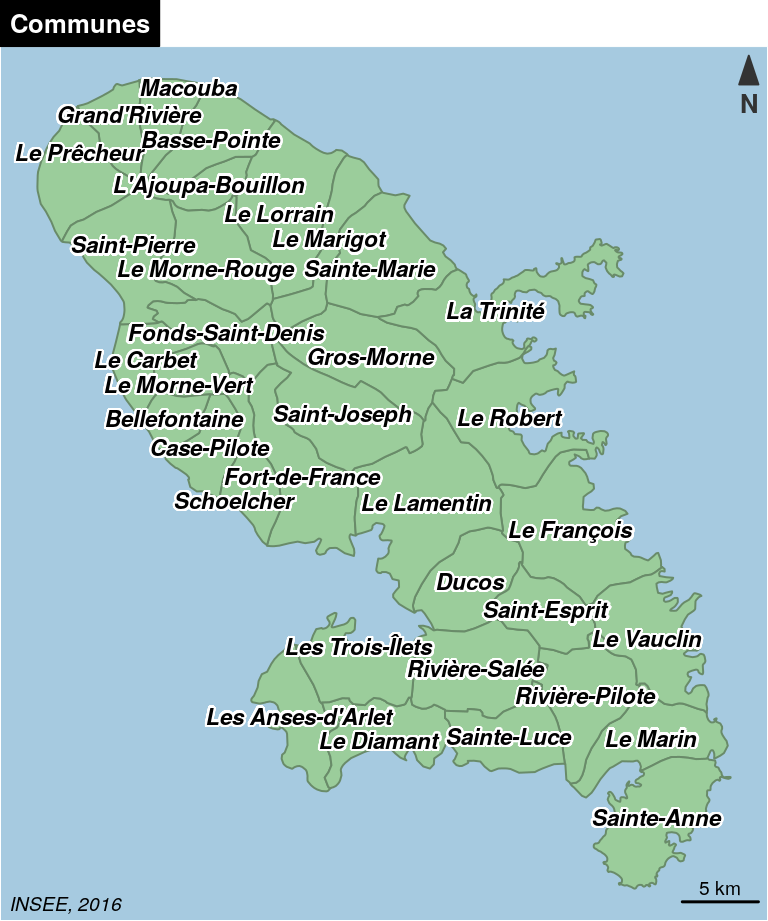
\includegraphics{Cartographie_avec_R_files/figure-latex/labs-1} \end{center}

\section{Autres fonctionnalités
utiles}\label{autres-fonctionnalites-utiles}

\subsection{Mise en page}\label{mise-en-page}

\subsubsection{Ajuster les marges d'une
figure}\label{ajuster-les-marges-dune-figure}

Pour modifier les marges d'une figure (carte ou autre) il faut utiliser
la fonction \texttt{par()} qui défini certains paramètres graphiques des
figures et son argument \texttt{mar}. La fonction \texttt{dev.off()}
efface tous les graphiques en mémoire et permet de réinitialiser les
valeurs par défaut.

\begin{Shaded}
\begin{Highlighting}[]
\CommentTok{# Modification de la couleur de fond des graphique}
\KeywordTok{par}\NormalTok{(}\DataTypeTok{bg=}\StringTok{"grey90"}\NormalTok{)}
\KeywordTok{plot}\NormalTok{(}\KeywordTok{st_geometry}\NormalTok{(mtq), }\DataTypeTok{main=}\StringTok{"Marges par défaut"}\NormalTok{)}
\end{Highlighting}
\end{Shaded}

\begin{center}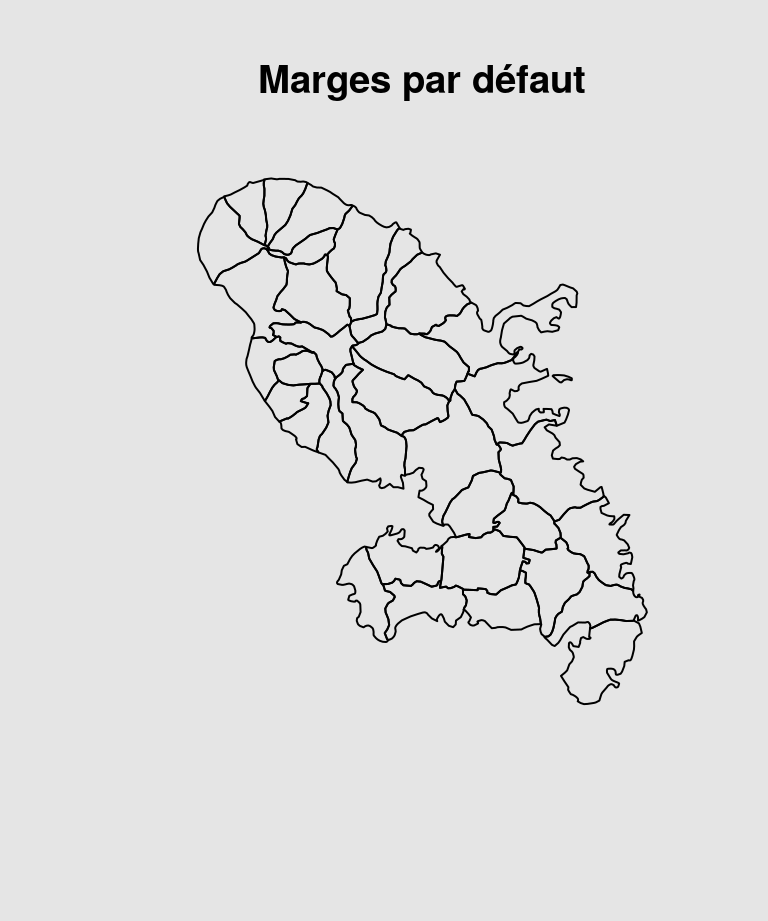
\includegraphics{Cartographie_avec_R_files/figure-latex/defmarg-1} \end{center}

\begin{Shaded}
\begin{Highlighting}[]
\CommentTok{# Modification des marges}
\KeywordTok{par}\NormalTok{(}\DataTypeTok{mar=}\KeywordTok{c}\NormalTok{(}\DecValTok{0}\NormalTok{,}\DecValTok{0}\NormalTok{,}\FloatTok{1.2}\NormalTok{,}\DecValTok{0}\NormalTok{))}
\KeywordTok{plot}\NormalTok{(}\KeywordTok{st_geometry}\NormalTok{(mtq), }\DataTypeTok{main=}\StringTok{"Marges paramétrées"}\NormalTok{)}
\end{Highlighting}
\end{Shaded}

\begin{center}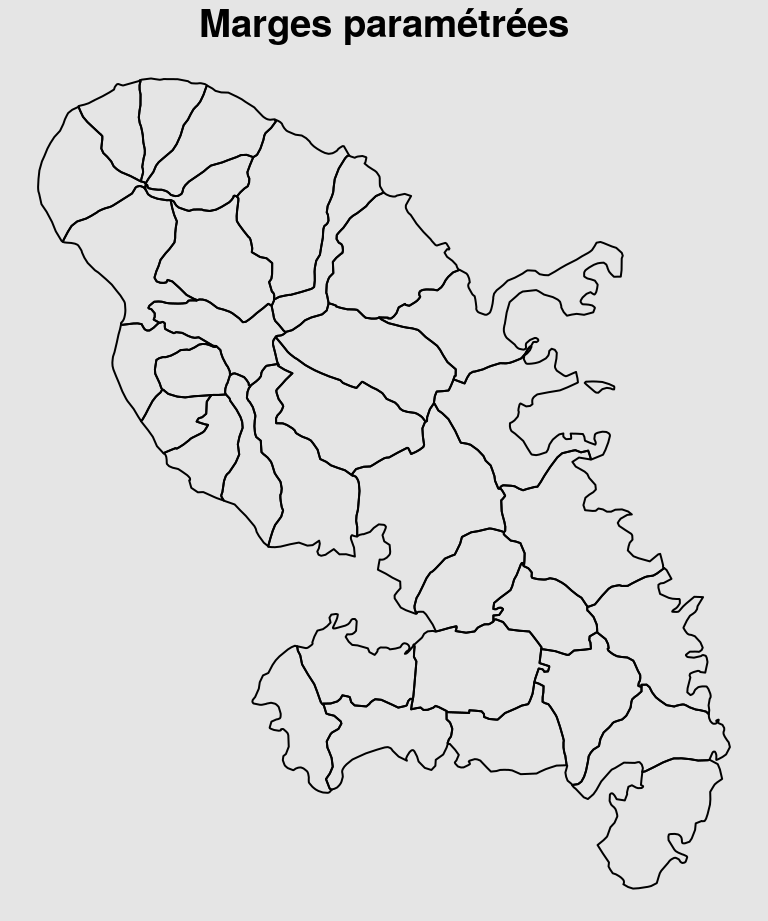
\includegraphics{Cartographie_avec_R_files/figure-latex/defmarg-2} \end{center}

\subsubsection{Centrer la carte sur une
région}\label{centrer-la-carte-sur-une-region}

Plusieurs solutions sont possible :

\begin{itemize}
\tightlist
\item
  Afficher une couche de la zone de zoom sans couleur pour le fond et
  les bordures puis afficher les couches que l'on souhaite afficher.
\end{itemize}

\begin{Shaded}
\begin{Highlighting}[]
\NormalTok{carbet <-}\StringTok{ }\NormalTok{mtq[mtq}\OperatorTok{$}\NormalTok{LIBGEO}\OperatorTok{==}\StringTok{"Le Carbet"}\NormalTok{,]}
\CommentTok{# affichage de la couche de zoom "invisible"}
\KeywordTok{plot}\NormalTok{(}
  \KeywordTok{st_geometry}\NormalTok{(carbet), }
  \DataTypeTok{col =} \OtherTok{NA}\NormalTok{, }
  \DataTypeTok{border =} \OtherTok{NA}\NormalTok{,}
  \DataTypeTok{bg =} \StringTok{"#A6CAE0"}
\NormalTok{)}
\CommentTok{# affichage des communes}
\KeywordTok{plot}\NormalTok{(}
  \KeywordTok{st_geometry}\NormalTok{(mtq), }
  \DataTypeTok{col =} \StringTok{"darkseagreen1"}\NormalTok{, }
  \DataTypeTok{border =} \StringTok{"darkseagreen4"}\NormalTok{, }
  \DataTypeTok{add=}\OtherTok{TRUE}
\NormalTok{)}
\CommentTok{# affichage de la couche d'intérêt}
\KeywordTok{plot}\NormalTok{(}
  \KeywordTok{st_geometry}\NormalTok{(carbet), }
  \DataTypeTok{col =} \StringTok{"darkseagreen3"}\NormalTok{, }
  \DataTypeTok{border =} \StringTok{"darkseagreen4"}\NormalTok{, }
  \DataTypeTok{lwd =} \DecValTok{2}\NormalTok{, }
  \DataTypeTok{add=}\OtherTok{TRUE}
\NormalTok{)}
\KeywordTok{layoutLayer}\NormalTok{(}
  \DataTypeTok{title =} \StringTok{"Le Carbet"}\NormalTok{, }
  \DataTypeTok{sources =} \StringTok{""}\NormalTok{,}
  \DataTypeTok{author =} \StringTok{""}\NormalTok{,}
  \DataTypeTok{scale =} \DecValTok{1}\NormalTok{,}
  \DataTypeTok{tabtitle =} \OtherTok{TRUE}\NormalTok{,}
  \DataTypeTok{frame=}\OtherTok{FALSE}
\NormalTok{)}
\end{Highlighting}
\end{Shaded}

\begin{center}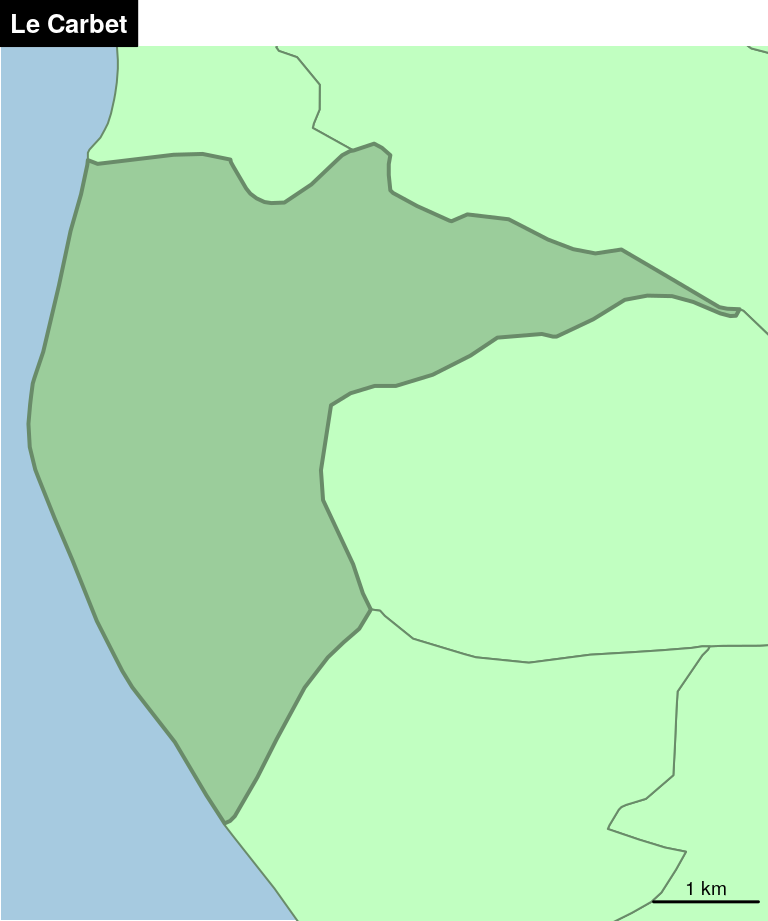
\includegraphics{Cartographie_avec_R_files/figure-latex/unnamed-chunk-16-1} \end{center}

\begin{itemize}
\tightlist
\item
  Utiliser les paramètres \texttt{xlim} et \texttt{ylim} de la fonction
  \texttt{plot()} aves les valeurs fournies par la fonction
  \texttt{st\_bbox()}
\end{itemize}

\begin{Shaded}
\begin{Highlighting}[]
\NormalTok{diams <-}\StringTok{ }\NormalTok{mtq[mtq}\OperatorTok{$}\NormalTok{LIBGEO}\OperatorTok{==}\StringTok{"Le Diamant"}\NormalTok{,]}
\NormalTok{diams_bb <-}\StringTok{ }\KeywordTok{st_bbox}\NormalTok{(diams)}
\CommentTok{# affichage des communes}
\KeywordTok{plot}\NormalTok{(}
  \KeywordTok{st_geometry}\NormalTok{(mtq), }
  \DataTypeTok{col =} \StringTok{"darkseagreen1"}\NormalTok{, }
  \DataTypeTok{border =} \StringTok{"darkseagreen4"}\NormalTok{, }
  \DataTypeTok{xlim =}\NormalTok{ diams_bb[}\KeywordTok{c}\NormalTok{(}\DecValTok{1}\NormalTok{,}\DecValTok{3}\NormalTok{)], }
  \DataTypeTok{ylim =}\NormalTok{ diams_bb[}\KeywordTok{c}\NormalTok{(}\DecValTok{2}\NormalTok{,}\DecValTok{4}\NormalTok{)], }
  \DataTypeTok{bg =} \StringTok{"#A6CAE0"}
\NormalTok{)}
\CommentTok{# affichage de la couche d'intérêt}
\KeywordTok{plot}\NormalTok{(}
  \KeywordTok{st_geometry}\NormalTok{(diams), }
  \DataTypeTok{col =} \StringTok{"darkseagreen3"}\NormalTok{, }
  \DataTypeTok{border =} \StringTok{"darkseagreen4"}\NormalTok{, }
  \DataTypeTok{lwd =} \DecValTok{2}\NormalTok{, }
  \DataTypeTok{add=}\OtherTok{TRUE}
\NormalTok{)}
\KeywordTok{layoutLayer}\NormalTok{(}
  \DataTypeTok{title =} \StringTok{"Le Diamant"}\NormalTok{, }
  \DataTypeTok{sources =} \StringTok{""}\NormalTok{,}
  \DataTypeTok{author =} \StringTok{""}\NormalTok{,}
  \DataTypeTok{scale =} \DecValTok{1}\NormalTok{,}
  \DataTypeTok{tabtitle =} \OtherTok{TRUE}\NormalTok{,}
  \DataTypeTok{frame=}\OtherTok{FALSE}
\NormalTok{)}
\end{Highlighting}
\end{Shaded}

\begin{center}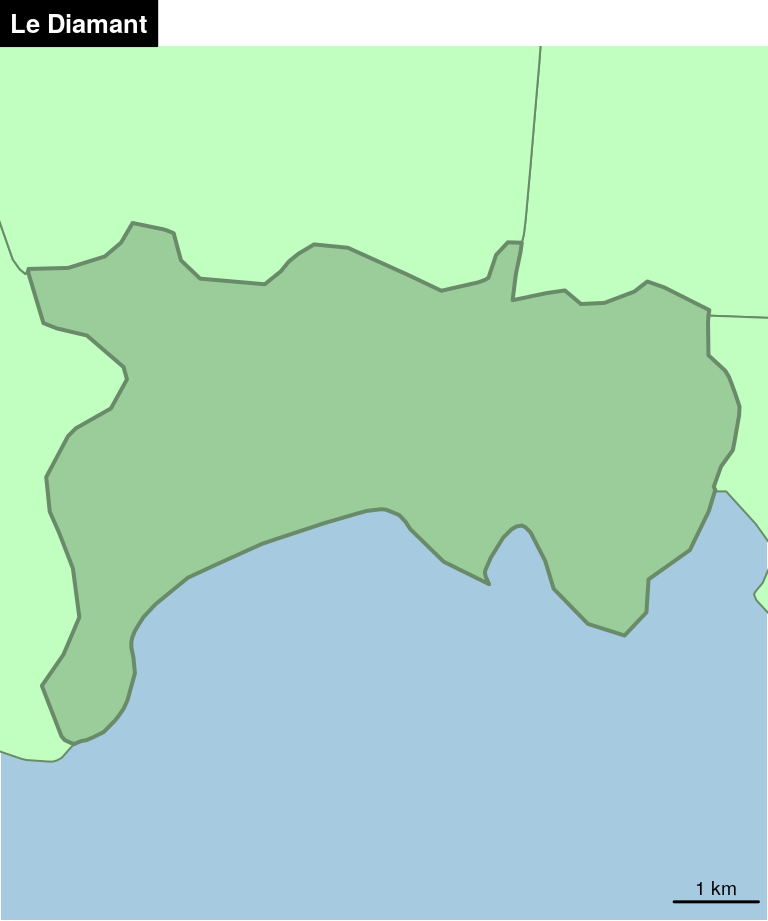
\includegraphics{Cartographie_avec_R_files/figure-latex/unnamed-chunk-17-1} \end{center}

\subsubsection{Afficher plusieurs cartes sur la même
figure}\label{afficher-plusieurs-cartes-sur-la-meme-figure}

Il faut ici utiliser l'argument \texttt{mfrow} de la fonction
\texttt{par()}. Le premier chiffre représente le nombre lignes et le
deuxième le nombre de colonnes.

\begin{Shaded}
\begin{Highlighting}[]
\CommentTok{# deux lignes et deux colonnes}
\KeywordTok{par}\NormalTok{(}\DataTypeTok{mfrow=}\KeywordTok{c}\NormalTok{(}\DecValTok{2}\NormalTok{,}\DecValTok{2}\NormalTok{))}
\KeywordTok{plot}\NormalTok{(}\KeywordTok{st_geometry}\NormalTok{(mtq), }\DataTypeTok{col=}\StringTok{"red"}\NormalTok{)}
\KeywordTok{plot}\NormalTok{(}\KeywordTok{st_geometry}\NormalTok{(mtq), }\DataTypeTok{col=}\StringTok{"blue"}\NormalTok{)}
\KeywordTok{plot}\NormalTok{(}\KeywordTok{st_geometry}\NormalTok{(mtq), }\DataTypeTok{col=}\StringTok{"green"}\NormalTok{)}
\KeywordTok{plot}\NormalTok{(}\KeywordTok{st_geometry}\NormalTok{(mtq), }\DataTypeTok{col=}\StringTok{"yellow"}\NormalTok{)}
\end{Highlighting}
\end{Shaded}

\begin{center}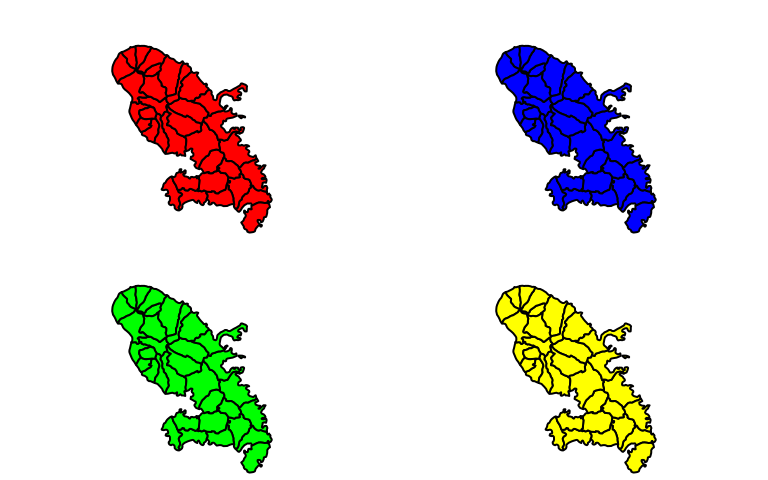
\includegraphics{Cartographie_avec_R_files/figure-latex/mfrow0-1} \end{center}

\begin{Shaded}
\begin{Highlighting}[]
\CommentTok{# une ligne et deux colonnes}
\KeywordTok{par}\NormalTok{(}\DataTypeTok{mfrow=}\KeywordTok{c}\NormalTok{(}\DecValTok{1}\NormalTok{,}\DecValTok{2}\NormalTok{), }\DataTypeTok{mar =} \KeywordTok{c}\NormalTok{(}\DecValTok{0}\NormalTok{,.}\DecValTok{2}\NormalTok{,}\FloatTok{1.2}\NormalTok{,.}\DecValTok{2}\NormalTok{))}
\CommentTok{# 1ere carte}
\NormalTok{carbet_bb <-}\StringTok{ }\KeywordTok{st_bbox}\NormalTok{(carbet)}
\KeywordTok{plot}\NormalTok{(}\KeywordTok{st_geometry}\NormalTok{(mtq), }\DataTypeTok{col =} \StringTok{"darkseagreen1"}\NormalTok{, }\DataTypeTok{border =} \StringTok{"darkseagreen4"}\NormalTok{, }
     \DataTypeTok{xlim =}\NormalTok{ carbet_bb[}\KeywordTok{c}\NormalTok{(}\DecValTok{1}\NormalTok{,}\DecValTok{3}\NormalTok{)], }\DataTypeTok{ylim =}\NormalTok{ carbet_bb[}\KeywordTok{c}\NormalTok{(}\DecValTok{2}\NormalTok{,}\DecValTok{4}\NormalTok{)], }\DataTypeTok{bg =} \StringTok{"#A6CAE0"}\NormalTok{)}
\KeywordTok{plot}\NormalTok{(}\KeywordTok{st_geometry}\NormalTok{(carbet), }\DataTypeTok{col =} \StringTok{"darkseagreen3"}\NormalTok{, }\DataTypeTok{border =} \StringTok{"darkseagreen4"}\NormalTok{, }
     \DataTypeTok{lwd =} \DecValTok{2}\NormalTok{, }\DataTypeTok{add=}\OtherTok{TRUE}\NormalTok{)}
\KeywordTok{layoutLayer}\NormalTok{(}\DataTypeTok{title =} \StringTok{"Le Carbet"}\NormalTok{, }\DataTypeTok{sources =} \StringTok{""}\NormalTok{, }\DataTypeTok{author =} \StringTok{""}\NormalTok{, }\DataTypeTok{scale =} \DecValTok{1}\NormalTok{, }
            \DataTypeTok{tabtitle =} \OtherTok{TRUE}\NormalTok{, }\DataTypeTok{frame=}\OtherTok{FALSE}\NormalTok{)}
\CommentTok{# 2eme carte }
\KeywordTok{plot}\NormalTok{(}\KeywordTok{st_geometry}\NormalTok{(mtq), }\DataTypeTok{col =} \StringTok{"darkseagreen1"}\NormalTok{, }\DataTypeTok{border =} \StringTok{"darkseagreen4"}\NormalTok{, }
     \DataTypeTok{xlim =}\NormalTok{ diams_bb[}\KeywordTok{c}\NormalTok{(}\DecValTok{1}\NormalTok{,}\DecValTok{3}\NormalTok{)], }\DataTypeTok{ylim =}\NormalTok{ diams_bb[}\KeywordTok{c}\NormalTok{(}\DecValTok{2}\NormalTok{,}\DecValTok{4}\NormalTok{)], }\DataTypeTok{bg =} \StringTok{"#A6CAE0"}\NormalTok{)}
\KeywordTok{plot}\NormalTok{(}\KeywordTok{st_geometry}\NormalTok{(diams), }\DataTypeTok{col =} \StringTok{"darkseagreen3"}\NormalTok{, }\DataTypeTok{border =} \StringTok{"darkseagreen4"}\NormalTok{, }
     \DataTypeTok{lwd =} \DecValTok{2}\NormalTok{, }\DataTypeTok{add=}\OtherTok{TRUE}\NormalTok{)}
\KeywordTok{layoutLayer}\NormalTok{(}\DataTypeTok{title =} \StringTok{"Le Diamant"}\NormalTok{, }\DataTypeTok{sources =} \StringTok{""}\NormalTok{, }\DataTypeTok{author =} \StringTok{""}\NormalTok{, }\DataTypeTok{scale =} \DecValTok{1}\NormalTok{, }
            \DataTypeTok{tabtitle =} \OtherTok{TRUE}\NormalTok{, }\DataTypeTok{frame=}\OtherTok{FALSE}\NormalTok{)}
\end{Highlighting}
\end{Shaded}

\begin{center}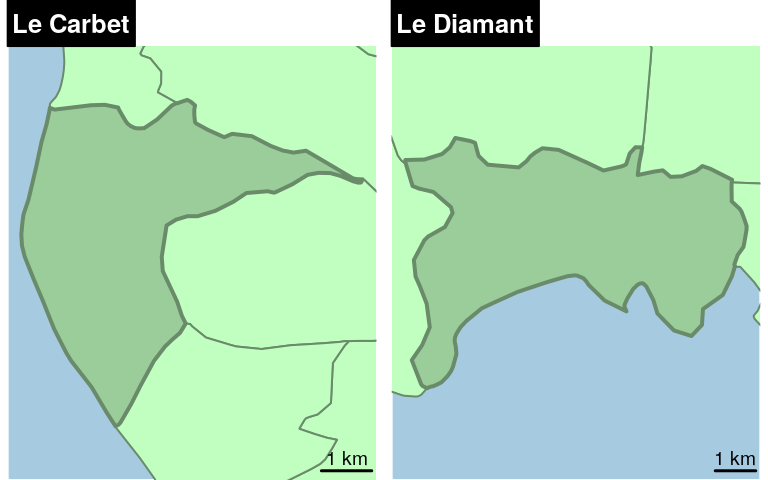
\includegraphics{Cartographie_avec_R_files/figure-latex/mfrow-1} \end{center}

\begin{Shaded}
\begin{Highlighting}[]
\CommentTok{# une ligne et deux colonnes}
\KeywordTok{par}\NormalTok{(}\DataTypeTok{mfrow=}\KeywordTok{c}\NormalTok{(}\DecValTok{2}\NormalTok{,}\DecValTok{1}\NormalTok{), }\DataTypeTok{mar =} \KeywordTok{c}\NormalTok{(}\FloatTok{0.2}\NormalTok{,}\DecValTok{0}\NormalTok{,}\FloatTok{1.4}\NormalTok{,}\DecValTok{0}\NormalTok{))}
\CommentTok{# 1ere carte}
\NormalTok{carbet_bb <-}\StringTok{ }\KeywordTok{st_bbox}\NormalTok{(carbet)}
\KeywordTok{plot}\NormalTok{(}\KeywordTok{st_geometry}\NormalTok{(mtq), }\DataTypeTok{col =} \StringTok{"darkseagreen1"}\NormalTok{, }\DataTypeTok{border =} \StringTok{"darkseagreen4"}\NormalTok{, }
     \DataTypeTok{xlim =}\NormalTok{ carbet_bb[}\KeywordTok{c}\NormalTok{(}\DecValTok{1}\NormalTok{,}\DecValTok{3}\NormalTok{)], }\DataTypeTok{ylim =}\NormalTok{ carbet_bb[}\KeywordTok{c}\NormalTok{(}\DecValTok{2}\NormalTok{,}\DecValTok{4}\NormalTok{)], }\DataTypeTok{bg =} \StringTok{"#A6CAE0"}\NormalTok{)}
\KeywordTok{plot}\NormalTok{(}\KeywordTok{st_geometry}\NormalTok{(carbet), }\DataTypeTok{col =} \StringTok{"darkseagreen3"}\NormalTok{, }\DataTypeTok{border =} \StringTok{"darkseagreen4"}\NormalTok{, }
     \DataTypeTok{lwd =} \DecValTok{2}\NormalTok{, }\DataTypeTok{add=}\OtherTok{TRUE}\NormalTok{)}
\KeywordTok{layoutLayer}\NormalTok{(}\DataTypeTok{title =} \StringTok{"Le Carbet"}\NormalTok{, }\DataTypeTok{sources =} \StringTok{""}\NormalTok{, }\DataTypeTok{author =} \StringTok{""}\NormalTok{, }\DataTypeTok{scale =} \DecValTok{1}\NormalTok{, }
            \DataTypeTok{tabtitle =} \OtherTok{TRUE}\NormalTok{, }\DataTypeTok{frame=}\OtherTok{FALSE}\NormalTok{)}
\CommentTok{# 2eme carte }
\KeywordTok{plot}\NormalTok{(}\KeywordTok{st_geometry}\NormalTok{(mtq), }\DataTypeTok{col =} \StringTok{"darkseagreen1"}\NormalTok{, }\DataTypeTok{border =} \StringTok{"darkseagreen4"}\NormalTok{, }
     \DataTypeTok{xlim =}\NormalTok{ diams_bb[}\KeywordTok{c}\NormalTok{(}\DecValTok{1}\NormalTok{,}\DecValTok{3}\NormalTok{)], }\DataTypeTok{ylim =}\NormalTok{ diams_bb[}\KeywordTok{c}\NormalTok{(}\DecValTok{2}\NormalTok{,}\DecValTok{4}\NormalTok{)], }\DataTypeTok{bg =} \StringTok{"#A6CAE0"}\NormalTok{)}
\KeywordTok{plot}\NormalTok{(}\KeywordTok{st_geometry}\NormalTok{(diams), }\DataTypeTok{col =} \StringTok{"darkseagreen3"}\NormalTok{, }\DataTypeTok{border =} \StringTok{"darkseagreen4"}\NormalTok{, }
     \DataTypeTok{lwd =} \DecValTok{2}\NormalTok{, }\DataTypeTok{add=}\OtherTok{TRUE}\NormalTok{)}
\KeywordTok{layoutLayer}\NormalTok{(}\DataTypeTok{title =} \StringTok{"Le Diamant"}\NormalTok{, }\DataTypeTok{sources =} \StringTok{""}\NormalTok{, }\DataTypeTok{author =} \StringTok{""}\NormalTok{, }\DataTypeTok{scale =} \DecValTok{1}\NormalTok{, }
            \DataTypeTok{tabtitle =} \OtherTok{TRUE}\NormalTok{, }\DataTypeTok{frame=}\OtherTok{FALSE}\NormalTok{)}
\end{Highlighting}
\end{Shaded}

\begin{center}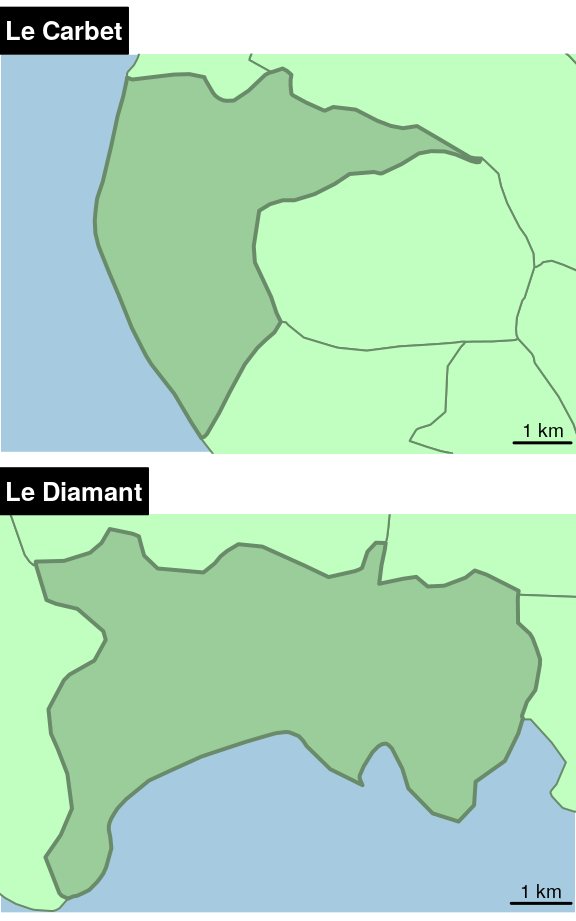
\includegraphics{Cartographie_avec_R_files/figure-latex/mfrow2-1} \end{center}

\subsubsection{Obtenir un ratio de figure
adapté}\label{obtenir-un-ratio-de-figure-adapte}

Il est assez difficile d'exporter des figures (cartes ou autres) dont le
ratio hauteur/largeur soit satisfaisant. Le ratio par défaut des figure
au format png est de 1 (480x480 pixels) :

\begin{Shaded}
\begin{Highlighting}[]
\KeywordTok{png}\NormalTok{(}\DataTypeTok{filename =} \StringTok{"img/martinique1.png"}\NormalTok{, }\DataTypeTok{res =} \DecValTok{96}\NormalTok{)}
\KeywordTok{par}\NormalTok{(}\DataTypeTok{mar =} \KeywordTok{c}\NormalTok{(}\DecValTok{0}\NormalTok{,}\DecValTok{0}\NormalTok{,}\FloatTok{1.2}\NormalTok{,}\DecValTok{0}\NormalTok{), }\DataTypeTok{bg =} \StringTok{"grey90"}\NormalTok{)}
\KeywordTok{plot}\NormalTok{(}\KeywordTok{st_geometry}\NormalTok{(mtq), }\DataTypeTok{bg =} \StringTok{"#A6CAE0"}\NormalTok{, }\DataTypeTok{col =} \StringTok{"#D1914D"}\NormalTok{, }\DataTypeTok{border =} \StringTok{"white"}\NormalTok{)}
\KeywordTok{layoutLayer}\NormalTok{(}\DataTypeTok{title =} \StringTok{"Martinique"}\NormalTok{, }\DataTypeTok{sources =} \StringTok{""}\NormalTok{, }\DataTypeTok{author =} \StringTok{""}\NormalTok{, }\DataTypeTok{scale =} \OtherTok{NULL}\NormalTok{)}
\KeywordTok{dev.off}\NormalTok{()}
\end{Highlighting}
\end{Shaded}

\begin{figure}
\centering
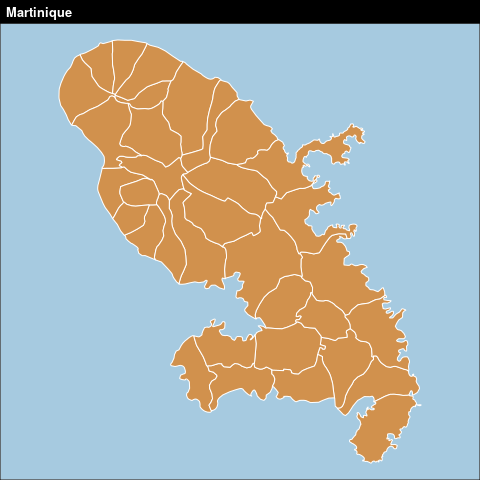
\includegraphics{img/martinique1.png}
\caption{}
\end{figure}

Sur cette carte beaucoup d'espace est perdu à l'est et à l'ouest de
l'ile.

La fonction \texttt{getFigDim()} de \texttt{cartography} permet de
choisir un ratio hauteur/largeur correspondant à l'emprise d'un objet
\texttt{sf} en prenant en compte une largeur (ou hauteur) fixée, les
paramètres de marges et la résolution souhaitée.

\begin{Shaded}
\begin{Highlighting}[]
\KeywordTok{getFigDim}\NormalTok{(}\DataTypeTok{x =}\NormalTok{ mtq, }\DataTypeTok{width =} \DecValTok{480}\NormalTok{, }\DataTypeTok{mar =} \KeywordTok{c}\NormalTok{(}\DecValTok{0}\NormalTok{,}\DecValTok{0}\NormalTok{,}\FloatTok{1.2}\NormalTok{,}\DecValTok{0}\NormalTok{), }\DataTypeTok{res =} \DecValTok{96}\NormalTok{)}
\end{Highlighting}
\end{Shaded}

\begin{verbatim}
[1] 480 583
\end{verbatim}

\begin{Shaded}
\begin{Highlighting}[]
\KeywordTok{png}\NormalTok{(}\DataTypeTok{filename =} \StringTok{"img/martinique2.png"}\NormalTok{, }\DataTypeTok{width =} \DecValTok{480}\NormalTok{, }\DataTypeTok{height =} \DecValTok{583}\NormalTok{, }\DataTypeTok{res =} \DecValTok{96}\NormalTok{)}
\KeywordTok{par}\NormalTok{(}\DataTypeTok{mar =} \KeywordTok{c}\NormalTok{(}\DecValTok{0}\NormalTok{,}\DecValTok{0}\NormalTok{,}\FloatTok{1.2}\NormalTok{,}\DecValTok{0}\NormalTok{), }\DataTypeTok{bg =} \StringTok{"grey90"}\NormalTok{)}
\KeywordTok{plot}\NormalTok{(}\KeywordTok{st_geometry}\NormalTok{(mtq), }\DataTypeTok{bg =} \StringTok{"#A6CAE0"}\NormalTok{, }\DataTypeTok{col =} \StringTok{"#D1914D"}\NormalTok{, }\DataTypeTok{border =} \StringTok{"white"}\NormalTok{)}
\KeywordTok{layoutLayer}\NormalTok{(}\DataTypeTok{title =} \StringTok{"Martinique"}\NormalTok{, }\DataTypeTok{sources =} \StringTok{""}\NormalTok{, }\DataTypeTok{author =} \StringTok{""}\NormalTok{, }\DataTypeTok{scale =} \OtherTok{NULL}\NormalTok{)}
\KeywordTok{dev.off}\NormalTok{()}
\end{Highlighting}
\end{Shaded}

\begin{figure}
\centering
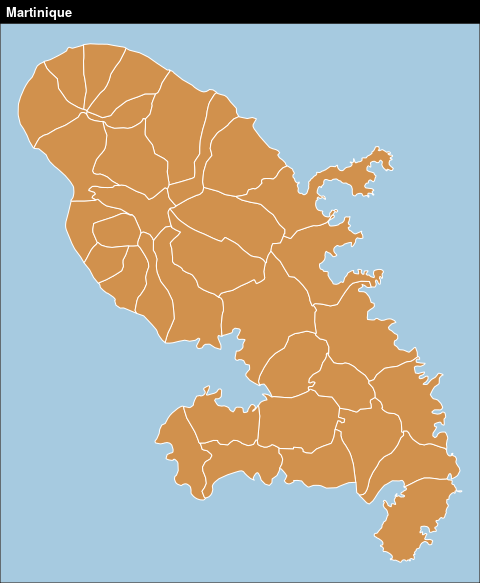
\includegraphics{img/martinique2.png}
\caption{}
\end{figure}

L'emprise de cette carte est exactement celle de l'île.

\subsubsection{Placer précisément un élément sur la
carte}\label{placer-precisement-un-element-sur-la-carte}

La fonction \texttt{locator()} permet de cliquer sur une figure et
d'obtenir les coordonnées d'un point dans le système de coordonnées de
la figure (de la carte).

\begin{Shaded}
\begin{Highlighting}[]
\KeywordTok{plot}\NormalTok{(}\KeywordTok{st_geometry}\NormalTok{(mtq), }\DataTypeTok{col =} \StringTok{"darkseagreen3"}\NormalTok{, }\DataTypeTok{border =} \StringTok{"darkseagreen4"}\NormalTok{, }
     \DataTypeTok{bg =} \StringTok{"#A6CAE0"}\NormalTok{)}
\KeywordTok{text}\NormalTok{(}\DataTypeTok{x =} \DecValTok{694019}\NormalTok{, }\DataTypeTok{y =} \DecValTok{1615161}\NormalTok{, }
     \DataTypeTok{labels =} \StringTok{"MER}\CharTok{\textbackslash{}n}\StringTok{DES}\CharTok{\textbackslash{}n}\StringTok{CARAÏBES"}\NormalTok{, }
     \DataTypeTok{col =} \StringTok{"#e3f1f9"}\NormalTok{, }\DataTypeTok{font =} \DecValTok{3}\NormalTok{, }\DataTypeTok{srt=}\DecValTok{20}\NormalTok{ )}
\end{Highlighting}
\end{Shaded}

\begin{center}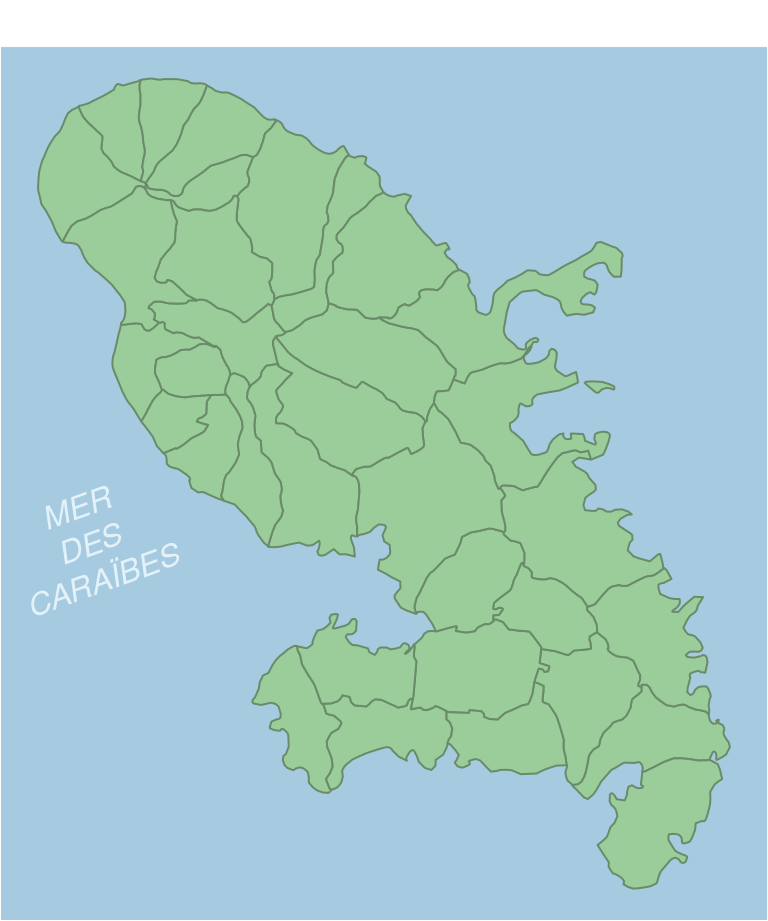
\includegraphics{Cartographie_avec_R_files/figure-latex/unnamed-chunk-21-1} \end{center}

\texttt{locator()}peut être utilisée sur la plupart des graphiques (pas
ceux produits avec \texttt{ggplot2}).

\subsection{Utiliser un fond de carte
OSM}\label{utiliser-un-fond-de-carte-osm}

La fonction \texttt{getTiles()} permet de télécharger des fonds de
cartes OSM et la fonction \texttt{tilesLayer()} permet de les afficher.

\begin{Shaded}
\begin{Highlighting}[]
\NormalTok{type <-}\StringTok{ }\KeywordTok{c}\NormalTok{( }\StringTok{"osm"}\NormalTok{, }\StringTok{"hotstyle"}\NormalTok{,  }\StringTok{"hikebike"}\NormalTok{, }\StringTok{"osmgrayscale"}\NormalTok{, }\StringTok{"stamenbw"}\NormalTok{,}
           \StringTok{"stamenwatercolor"}\NormalTok{, }\StringTok{"cartodark"}\NormalTok{, }\StringTok{"cartolight"}\NormalTok{)}
\KeywordTok{par}\NormalTok{(}\DataTypeTok{mar =} \KeywordTok{c}\NormalTok{(}\DecValTok{0}\NormalTok{,}\DecValTok{0}\NormalTok{,}\DecValTok{0}\NormalTok{,}\DecValTok{0}\NormalTok{), }\DataTypeTok{mfrow =} \KeywordTok{c}\NormalTok{(}\DecValTok{3}\NormalTok{,}\DecValTok{3}\NormalTok{))}
\ControlFlowTok{for}\NormalTok{ (i }\ControlFlowTok{in}\NormalTok{ type)\{}
  \KeywordTok{tilesLayer}\NormalTok{(}\KeywordTok{getTiles}\NormalTok{(}\DataTypeTok{x =}\NormalTok{ mtq, }\DataTypeTok{type =}\NormalTok{ i, }\DataTypeTok{crop=}\OtherTok{TRUE}\NormalTok{))}
  \KeywordTok{mtext}\NormalTok{(}\DataTypeTok{side =} \DecValTok{3}\NormalTok{, }\DataTypeTok{line =} \OperatorTok{-}\FloatTok{1.5}\NormalTok{, }\DataTypeTok{text =}\NormalTok{ i, }\DataTypeTok{col=}\StringTok{"red"}\NormalTok{)}
\NormalTok{\}}
\end{Highlighting}
\end{Shaded}

\begin{center}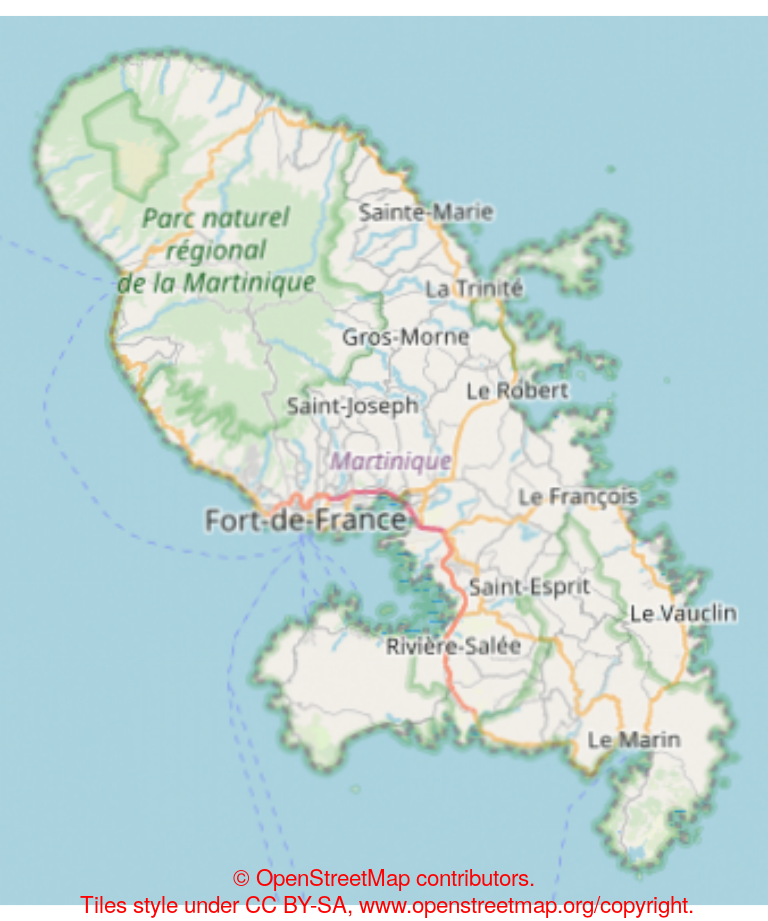
\includegraphics{Cartographie_avec_R_files/figure-latex/osmdisplay-1} \end{center}

\subsection{Créer un effet crayonné}\label{creer-un-effet-crayonne}

\begin{Shaded}
\begin{Highlighting}[]
\KeywordTok{library}\NormalTok{(sf)}
\NormalTok{mtq_pencil <-}\StringTok{ }\KeywordTok{getPencilLayer}\NormalTok{(}\DataTypeTok{x =}\NormalTok{ mtq)}
\KeywordTok{typoLayer}\NormalTok{(}
  \DataTypeTok{x =}\NormalTok{ mtq_pencil, }
  \DataTypeTok{var=}\StringTok{"STATUT"}\NormalTok{, }
  \DataTypeTok{col =} \KeywordTok{c}\NormalTok{(}\StringTok{"aquamarine4"}\NormalTok{, }\StringTok{"yellow3"}\NormalTok{,}\StringTok{"wheat"}\NormalTok{),}
  \DataTypeTok{legend.values.order =} \KeywordTok{c}\NormalTok{(}\StringTok{"Préfecture de région"}\NormalTok{,}
                          \StringTok{"Sous-préfecture"}\NormalTok{, }
                          \StringTok{"Commune simple"}\NormalTok{),}
  \DataTypeTok{legend.pos =} \StringTok{"topright"}\NormalTok{,}
  \DataTypeTok{legend.title.txt =} \StringTok{"Status"}
\NormalTok{)}
\KeywordTok{plot}\NormalTok{(}\KeywordTok{st_geometry}\NormalTok{(mtq), }\DataTypeTok{add =} \OtherTok{TRUE}\NormalTok{, }\DataTypeTok{ldy=}\DecValTok{2}\NormalTok{)}
\KeywordTok{layoutLayer}\NormalTok{(}\DataTypeTok{title =} \StringTok{"Statut Administratif"}\NormalTok{,}\DataTypeTok{tabtitle=}\OtherTok{TRUE}\NormalTok{,}
            \DataTypeTok{author=} \StringTok{"INSEE, 2016"}\NormalTok{, }\DataTypeTok{sources=}\StringTok{""}\NormalTok{, }
            \DataTypeTok{frame=}\OtherTok{FALSE}\NormalTok{, }\DataTypeTok{scale =} \DecValTok{5}\NormalTok{)}
\KeywordTok{north}\NormalTok{(}\DataTypeTok{pos =} \StringTok{"topleft"}\NormalTok{)}
\end{Highlighting}
\end{Shaded}

\begin{center}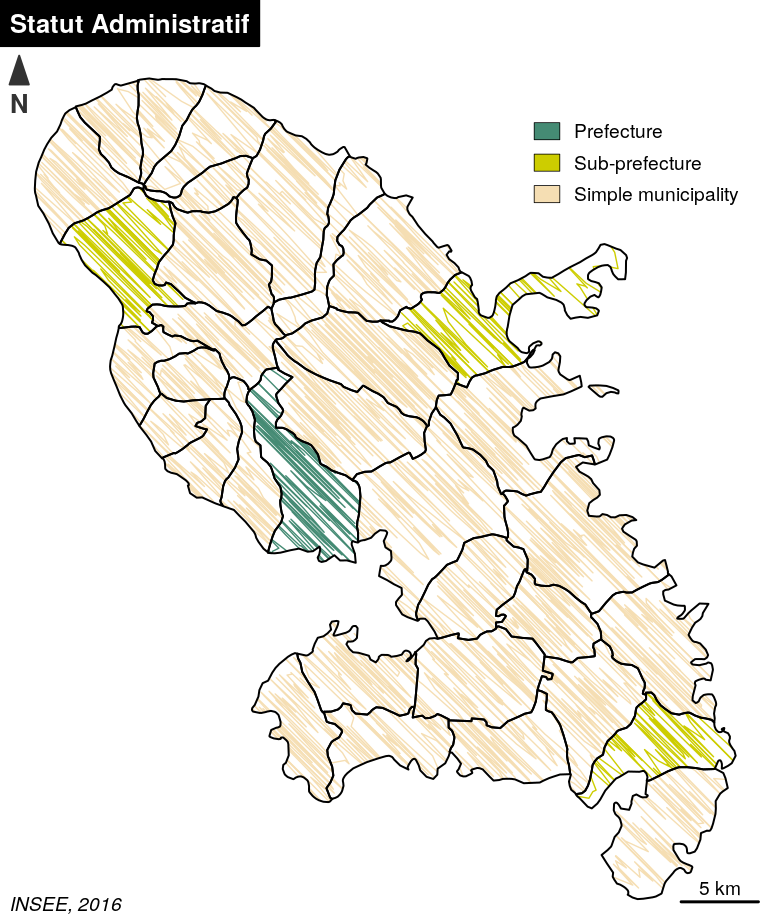
\includegraphics{Cartographie_avec_R_files/figure-latex/pencil-1} \end{center}

\subsection{Ajouter un ombrage à une
couche}\label{ajouter-un-ombrage-a-une-couche}

\begin{Shaded}
\begin{Highlighting}[]
\KeywordTok{plot}\NormalTok{(}\KeywordTok{st_geometry}\NormalTok{(mtq) }\OperatorTok{+}\StringTok{ }\KeywordTok{c}\NormalTok{(}\DecValTok{500}\NormalTok{, }\OperatorTok{-}\DecValTok{500}\NormalTok{), }
     \DataTypeTok{col =} \StringTok{"grey50"}\NormalTok{, }\DataTypeTok{border =} \OtherTok{NA}\NormalTok{, }\DataTypeTok{bg =} \StringTok{"lightblue1"}\NormalTok{)}
\KeywordTok{plot}\NormalTok{(}\KeywordTok{st_geometry}\NormalTok{(mtq), }\DataTypeTok{col=}\StringTok{"darkseagreen3"}\NormalTok{, }\DataTypeTok{border=}\StringTok{"darkseagreen4"}\NormalTok{, }\DataTypeTok{add=}\OtherTok{TRUE}\NormalTok{)}
\KeywordTok{layoutLayer}\NormalTok{(}\DataTypeTok{title =} \StringTok{"Communes"}\NormalTok{,}\DataTypeTok{tabtitle=}\OtherTok{TRUE}\NormalTok{,}
            \DataTypeTok{author=} \StringTok{"INSEE, 2016"}\NormalTok{, }\DataTypeTok{sources=}\StringTok{""}\NormalTok{, }\DataTypeTok{north=}\OtherTok{TRUE}\NormalTok{,  }
            \DataTypeTok{frame=}\OtherTok{FALSE}\NormalTok{, }\DataTypeTok{scale =} \DecValTok{5}\NormalTok{)}
\end{Highlighting}
\end{Shaded}

\begin{center}\includegraphics{Cartographie_avec_R_files/figure-latex/shadow-1} \end{center}

\subsection{Création de cartons}\label{creation-de-cartons}

Le package \texttt{mapinsetr}\citep{R-mapinsetr} est dédié à la crétion
de cartons cartographiques. Il n'est pas sur le CRAN pour l'instant,
mais on peut l'installer via le package \texttt{remotes}.

\begin{Shaded}
\begin{Highlighting}[]
\NormalTok{remotes}\OperatorTok{::}\KeywordTok{install_github}\NormalTok{(}\StringTok{"riatelab/mapinsetr"}\NormalTok{)}
\end{Highlighting}
\end{Shaded}

\texttt{mapinsetr} permet de découper, redimensionner et déplacer une
zone d'un fond de carte.

\begin{Shaded}
\begin{Highlighting}[]
\KeywordTok{library}\NormalTok{(mapinsetr)}
\KeywordTok{library}\NormalTok{(cartography)}
\KeywordTok{library}\NormalTok{(sf)}
\NormalTok{mtq <-}\StringTok{ }\KeywordTok{st_read}\NormalTok{(}\StringTok{"data/martinique.shp"}\NormalTok{, }\DataTypeTok{quiet =} \OtherTok{TRUE}\NormalTok{)}
\NormalTok{resto <-}\StringTok{ }\KeywordTok{st_read}\NormalTok{(}\StringTok{"data/resto.gpkg"}\NormalTok{, }\DataTypeTok{quiet =} \OtherTok{TRUE}\NormalTok{)}
\CommentTok{# Création d'un masque}
\NormalTok{box_FDF <-}\StringTok{ }\KeywordTok{create_mask}\NormalTok{(}\DataTypeTok{bb =} \KeywordTok{c}\NormalTok{(}\DecValTok{706880}\NormalTok{, }\DecValTok{1615030}\NormalTok{, }\DecValTok{708650}\NormalTok{, }\DecValTok{1616870}\NormalTok{), }
                       \DataTypeTok{prj =} \KeywordTok{st_crs}\NormalTok{(mtq))}
\CommentTok{# Découpage, déplacement et redimentionnement des couches sous le masque}
\NormalTok{zbox_FDF <-}\StringTok{ }\KeywordTok{move_and_resize}\NormalTok{(}
  \DataTypeTok{x =}\NormalTok{ box_FDF, }
  \DataTypeTok{mask =}\NormalTok{ box_FDF, }
  \DataTypeTok{xy =} \KeywordTok{c}\NormalTok{(}\DecValTok{689000}\NormalTok{, }\DecValTok{1603000}\NormalTok{), }
  \DataTypeTok{k =} \DecValTok{7}
\NormalTok{)}
\NormalTok{zmtq_FDF <-}\StringTok{ }\KeywordTok{move_and_resize}\NormalTok{(}
  \DataTypeTok{x =}\NormalTok{ mtq, }
  \DataTypeTok{mask =}\NormalTok{ box_FDF, }
  \DataTypeTok{xy =} \KeywordTok{c}\NormalTok{(}\DecValTok{689000}\NormalTok{, }\DecValTok{1603000}\NormalTok{), }
  \DataTypeTok{k =} \DecValTok{7}
\NormalTok{)}
\NormalTok{zresto_FDF <-}\StringTok{ }\KeywordTok{move_and_resize}\NormalTok{(}
  \DataTypeTok{x =}\NormalTok{ resto, }
  \DataTypeTok{mask =}\NormalTok{ box_FDF, }
  \DataTypeTok{xy =} \KeywordTok{c}\NormalTok{(}\DecValTok{689000}\NormalTok{, }\DecValTok{1603000}\NormalTok{), }
  \DataTypeTok{k =} \DecValTok{7}
\NormalTok{)}
\CommentTok{# Affichage de la carte et des couhes crées}
\KeywordTok{plot}\NormalTok{(}\KeywordTok{st_geometry}\NormalTok{(mtq), }\DataTypeTok{col =} \StringTok{"lightblue4"}\NormalTok{, }\DataTypeTok{border =} \StringTok{"lightblue3"}\NormalTok{, }
     \DataTypeTok{bg =} \StringTok{"lightblue1"}\NormalTok{)}
\KeywordTok{plot}\NormalTok{(}\KeywordTok{st_geometry}\NormalTok{(resto), }\DataTypeTok{add=}\NormalTok{T, }\DataTypeTok{pch=}\DecValTok{20}\NormalTok{, }\DataTypeTok{col =} \StringTok{"#330A5FFF"}\NormalTok{, }\DataTypeTok{cex =} \FloatTok{0.5}\NormalTok{)}
\KeywordTok{plot}\NormalTok{(}\KeywordTok{st_geometry}\NormalTok{(box_FDF), }\DataTypeTok{border =} \StringTok{"red"}\NormalTok{, }\DataTypeTok{add =}\NormalTok{ T, }\DataTypeTok{lwd =} \DecValTok{2}\NormalTok{)}
\KeywordTok{plot}\NormalTok{(}\KeywordTok{st_geometry}\NormalTok{(zmtq_FDF), }\DataTypeTok{col =} \StringTok{"lightblue4"}\NormalTok{, }\DataTypeTok{border =} \StringTok{"lightblue3"}\NormalTok{, }\DataTypeTok{add=}\OtherTok{TRUE}\NormalTok{)}
\KeywordTok{plot}\NormalTok{(}\KeywordTok{st_geometry}\NormalTok{(zresto_FDF), }\DataTypeTok{add=}\OtherTok{TRUE}\NormalTok{, }\DataTypeTok{pch=}\DecValTok{20}\NormalTok{, }\DataTypeTok{col =} \StringTok{"#330A5FFF"}\NormalTok{, }\DataTypeTok{cex =} \FloatTok{0.5}\NormalTok{)}
\KeywordTok{plot}\NormalTok{(}\KeywordTok{st_geometry}\NormalTok{(zbox_FDF), }\DataTypeTok{border =} \StringTok{"red"}\NormalTok{, }\DataTypeTok{add =}\NormalTok{ T, }\DataTypeTok{lwd =} \DecValTok{2}\NormalTok{)}
\KeywordTok{layoutLayer}\NormalTok{(}\DataTypeTok{title =} \StringTok{"Carte initiale + couches créées"}\NormalTok{,}\DataTypeTok{tabtitle=}\OtherTok{TRUE}\NormalTok{,}
            \DataTypeTok{author=} \StringTok{"INSEE, 2016"}\NormalTok{, }\DataTypeTok{sources=}\StringTok{""}\NormalTok{, }\DataTypeTok{north=}\OtherTok{TRUE}\NormalTok{,  }
            \DataTypeTok{frame=}\OtherTok{FALSE}\NormalTok{, }\DataTypeTok{scale =} \DecValTok{5}\NormalTok{)}
\end{Highlighting}
\end{Shaded}

\begin{center}\includegraphics{Cartographie_avec_R_files/figure-latex/inset1-1} \end{center}

\begin{Shaded}
\begin{Highlighting}[]
\CommentTok{# Création de couches unqiues comprenant le zoom}
\NormalTok{resto <-}\StringTok{ }\KeywordTok{inset_rbinder}\NormalTok{(}\DataTypeTok{l =} \KeywordTok{list}\NormalTok{(resto, zresto_FDF))}
\NormalTok{mtq <-}\StringTok{ }\KeywordTok{inset_rbinder}\NormalTok{(}\DataTypeTok{l =} \KeywordTok{list}\NormalTok{(mtq, zmtq_FDF))}
\NormalTok{box <-}\StringTok{ }\KeywordTok{inset_rbinder}\NormalTok{(}\DataTypeTok{l =} \KeywordTok{list}\NormalTok{(box_FDF, zbox_FDF))}
\KeywordTok{plot}\NormalTok{(}\KeywordTok{st_geometry}\NormalTok{(mtq), }\DataTypeTok{col =} \StringTok{"lightblue4"}\NormalTok{, }\DataTypeTok{border =} \StringTok{"lightblue3"}\NormalTok{, }
     \DataTypeTok{bg =} \StringTok{"lightblue1"}\NormalTok{)}
\KeywordTok{plot}\NormalTok{(}\KeywordTok{st_geometry}\NormalTok{(resto), }\DataTypeTok{add=}\NormalTok{T, }\DataTypeTok{pch=}\DecValTok{20}\NormalTok{, }\DataTypeTok{col =} \StringTok{"#330A5FFF"}\NormalTok{, }\DataTypeTok{cex =} \FloatTok{0.5}\NormalTok{)}
\KeywordTok{plot}\NormalTok{(}\KeywordTok{st_geometry}\NormalTok{(box), }\DataTypeTok{border =} \StringTok{"red"}\NormalTok{, }\DataTypeTok{add =}\NormalTok{ T, }\DataTypeTok{lwd =} \DecValTok{2}\NormalTok{)}
\KeywordTok{layoutLayer}\NormalTok{(}\DataTypeTok{title =} \StringTok{"Carte finale avec carton"}\NormalTok{,}\DataTypeTok{tabtitle=}\OtherTok{TRUE}\NormalTok{,}
            \DataTypeTok{author=} \StringTok{"INSEE, 2016"}\NormalTok{, }\DataTypeTok{sources=}\StringTok{""}\NormalTok{, }\DataTypeTok{north=}\OtherTok{TRUE}\NormalTok{,  }
            \DataTypeTok{frame=}\OtherTok{FALSE}\NormalTok{, }\DataTypeTok{scale =} \DecValTok{5}\NormalTok{)}
\end{Highlighting}
\end{Shaded}

\begin{center}\includegraphics{Cartographie_avec_R_files/figure-latex/inset1-2} \end{center}

\hypertarget{chapitre3}{\chapter{Cartographie thématique
avancée}\label{chapitre3}}

\section{Les cartes de
discontinuités}\label{les-cartes-de-discontinuites}

Ce type de représentation permet de souligner cartographiquement les
discontinuités territoriales d'un phénomène. L'accent est porté sur ce
qui distingue des territoires. Pour chaque frontière nous calculons le
rapports ou la différence des valeurs des polygones de part et d'autre.
Puis nous représentons la frontière par un figuré d'autant plus épais
que la différence est forte. Il est souvent bénéfique de coupler ce type
de représentation à une représentation choroplèthe (pour comprendre le
sens des discontinuités).

\begin{center}\includegraphics[width=13.89in]{img/discmet} \end{center}

\begin{center}\includegraphics[width=11.67in]{img/disc2} \end{center}

\BeginKnitrBlock{rmdmoins}
Ces cartes ne sont pas évidentes à paramétrer. Le choix des critères
(seuil, type de différences\ldots{}) influence fortement la
représentation. En fonction du maillage utilisé la lisibilité de la
carte peut être faible.
\EndKnitrBlock{rmdmoins}

\BeginKnitrBlock{rmdplus}
Ces représentations sont très puissantes pour montrer les inégalités.
\EndKnitrBlock{rmdplus}

La fonctions \texttt{getBorder()} du package \texttt{cartography} permet
de construire une couche des frontières terrestres. La fonction
\texttt{discLayer()} permet d'afficher les discontinuités.

\begin{Shaded}
\begin{Highlighting}[]
\KeywordTok{library}\NormalTok{(sf)}
\KeywordTok{library}\NormalTok{(cartography)}
\NormalTok{mtq <-}\StringTok{ }\KeywordTok{st_read}\NormalTok{(}\StringTok{"data/martinique.shp"}\NormalTok{, }\DataTypeTok{quiet =} \OtherTok{TRUE}\NormalTok{)}
\CommentTok{# Get borders}
\NormalTok{mtq_bord <-}\StringTok{ }\KeywordTok{getBorders}\NormalTok{(}\DataTypeTok{x =}\NormalTok{ mtq)}
\CommentTok{# Plot polygons}
\KeywordTok{plot}\NormalTok{(}\KeywordTok{st_geometry}\NormalTok{(mtq), }\DataTypeTok{border =} \OtherTok{NA}\NormalTok{, }\DataTypeTok{col =} \StringTok{"grey60"}\NormalTok{)}
\CommentTok{# Plot borders}
\KeywordTok{plot}\NormalTok{(}
  \KeywordTok{st_geometry}\NormalTok{(mtq_bord), }
  \DataTypeTok{col =} \KeywordTok{sample}\NormalTok{(}\DataTypeTok{x =} \KeywordTok{rainbow}\NormalTok{(}\KeywordTok{nrow}\NormalTok{(mtq_bord))), }
  \DataTypeTok{lwd =} \DecValTok{3}\NormalTok{, }
  \DataTypeTok{add =} \OtherTok{TRUE}
\NormalTok{)}
\KeywordTok{layoutLayer}\NormalTok{(}\StringTok{"Frontières inter-communales"}\NormalTok{,}\DataTypeTok{tabtitle=}\OtherTok{TRUE}\NormalTok{, }\DataTypeTok{north =} \OtherTok{TRUE}\NormalTok{,}
            \DataTypeTok{author=} \StringTok{"INSEE 2016"}\NormalTok{, }\DataTypeTok{sources=}\StringTok{""}\NormalTok{, }\DataTypeTok{frame=}\OtherTok{FALSE}\NormalTok{, }\DataTypeTok{scale =} \DecValTok{5}\NormalTok{)}
\end{Highlighting}
\end{Shaded}

\begin{center}\includegraphics{Cartographie_avec_R_files/figure-latex/disc-1} \end{center}

\begin{Shaded}
\begin{Highlighting}[]
\NormalTok{mtq}\OperatorTok{$}\NormalTok{emp_share <-}\StringTok{ }\DecValTok{100} \OperatorTok{*}\StringTok{ }\NormalTok{mtq}\OperatorTok{$}\NormalTok{C13_CS5}\OperatorTok{/}\NormalTok{mtq}\OperatorTok{$}\NormalTok{C13_POP}
\CommentTok{# Plot this share}
\KeywordTok{choroLayer}\NormalTok{(}
  \DataTypeTok{x =}\NormalTok{ mtq, }
  \DataTypeTok{var =} \StringTok{"emp_share"}\NormalTok{, }
  \DataTypeTok{border =} \OtherTok{NA}\NormalTok{, }
  \DataTypeTok{method =} \StringTok{'quantile'}\NormalTok{, }
  \DataTypeTok{nclass =} \DecValTok{6}\NormalTok{, }
  \DataTypeTok{legend.values.rnd =} \DecValTok{1}\NormalTok{, }
  \DataTypeTok{legend.pos =} \StringTok{"topright"}\NormalTok{, }
  \DataTypeTok{legend.title.txt =} \StringTok{"Part des employés}\CharTok{\textbackslash{}n}\StringTok{dans la population agée}\CharTok{\textbackslash{}n}\StringTok{de 15 ans et plus"}\NormalTok{ )}
\CommentTok{# Plot discontinuities}
\KeywordTok{discLayer}\NormalTok{(}
  \DataTypeTok{x =}\NormalTok{ mtq_bord, }
  \DataTypeTok{df =}\NormalTok{ mtq,}
  \DataTypeTok{var =} \StringTok{"emp_share"}\NormalTok{, }
  \DataTypeTok{col=}\StringTok{"darkred"}\NormalTok{, }
  \DataTypeTok{nclass=}\DecValTok{3}\NormalTok{, }
  \DataTypeTok{method=}\StringTok{"quantile"}\NormalTok{, }
  \DataTypeTok{threshold =} \FloatTok{0.5}\NormalTok{, }
  \DataTypeTok{sizemin =} \FloatTok{0.5}\NormalTok{, }
  \DataTypeTok{sizemax =} \DecValTok{8}\NormalTok{, }
  \DataTypeTok{type =} \StringTok{"abs"}\NormalTok{, }
  \DataTypeTok{legend.values.rnd =} \DecValTok{1}\NormalTok{,}
  \DataTypeTok{legend.title.txt =} \StringTok{"Discontinuités}\CharTok{\textbackslash{}n}\StringTok{(différences absolues)"}\NormalTok{,}
  \DataTypeTok{legend.pos =} \StringTok{"bottomleft"}\NormalTok{, }\DataTypeTok{add=}\OtherTok{TRUE}
\NormalTok{)}
\KeywordTok{layoutLayer}\NormalTok{(}\StringTok{"Discontinuités - Part des employés"}\NormalTok{,}\DataTypeTok{tabtitle=}\OtherTok{TRUE}\NormalTok{, }
            \DataTypeTok{author=} \StringTok{"INSEE 2016"}\NormalTok{, }\DataTypeTok{sources=}\StringTok{""}\NormalTok{, }\DataTypeTok{frame=}\OtherTok{FALSE}\NormalTok{, }\DataTypeTok{scale =} \DecValTok{5}\NormalTok{)}
\KeywordTok{north}\NormalTok{(}\DataTypeTok{pos =} \StringTok{"topleft"}\NormalTok{)}
\end{Highlighting}
\end{Shaded}

\begin{center}\includegraphics{Cartographie_avec_R_files/figure-latex/disc2-1} \end{center}

\section{Les grilles régulières}\label{les-grilles-regulieres}

La méthode du carroyage consiste à découper l'espace géographique en un
maillage formé de carrés réguliers dans une projection donnée. La donnée
est répartie sur ce quadrillage régulier au prorata de la surface
représentée. Le quadrillage permet ainsi de s'affranchir des mailles
administratives.

\begin{center}\includegraphics[width=13.89in]{img/caromet} \end{center}

\begin{center}\includegraphics[width=8.33in]{img/grid} \end{center}

\begin{center}\includegraphics[width=8.33in]{img/grid} \end{center}

\BeginKnitrBlock{rmdmoins}
Ces représentation induisent une perte de précision. Les maillages
produit n'ont pas de signification. La version simple (les valeurs sont
redistribuées au prorata de la surface), implique une equirépartition du
phénomène dans chaque unités.
\EndKnitrBlock{rmdmoins}

\BeginKnitrBlock{rmdplus}
La comparaison de maillages différents, à plusieurs dates ou de
différentes sources est rendue possible.
\EndKnitrBlock{rmdplus}

La fonction \texttt{getGridLayer()} du package \texttt{cartography}
permet de construire ces grilles régulières.

\begin{Shaded}
\begin{Highlighting}[]
\KeywordTok{library}\NormalTok{(sf)}
\KeywordTok{library}\NormalTok{(cartography)}
\KeywordTok{library}\NormalTok{(sp)}
\NormalTok{mtq <-}\StringTok{ }\KeywordTok{st_read}\NormalTok{(}\StringTok{"data/martinique.shp"}\NormalTok{, }\DataTypeTok{quiet =} \OtherTok{TRUE}\NormalTok{)}
\CommentTok{# Plot dentsity of population }
\NormalTok{mtq}\OperatorTok{$}\NormalTok{dens <-}\StringTok{ }\NormalTok{mtq}\OperatorTok{$}\NormalTok{P13_POP }\OperatorTok{/}\StringTok{ }\NormalTok{(}\KeywordTok{st_area}\NormalTok{(mtq) }\OperatorTok{/}\StringTok{ }\NormalTok{(}\DecValTok{1000} \OperatorTok{*}\StringTok{ }\DecValTok{1000}\NormalTok{)) }
\NormalTok{bks <-}\StringTok{ }\KeywordTok{getBreaks}\NormalTok{(}\DataTypeTok{v =}\NormalTok{ mtq}\OperatorTok{$}\NormalTok{dens, }\DataTypeTok{method =} \StringTok{"q6"}\NormalTok{)}
\NormalTok{cols <-}\StringTok{ }\KeywordTok{carto.pal}\NormalTok{(}\DataTypeTok{pal1 =} \StringTok{"taupe.pal"}\NormalTok{, }\DataTypeTok{n1 =} \DecValTok{6}\NormalTok{)}
\KeywordTok{choroLayer}\NormalTok{(}
  \DataTypeTok{x =}\NormalTok{ mtq, }
  \DataTypeTok{var =} \StringTok{"dens"}\NormalTok{, }
  \DataTypeTok{breaks =}\NormalTok{ bks, }
  \DataTypeTok{border =} \StringTok{"burlywood3"}\NormalTok{, }
  \DataTypeTok{col =}\NormalTok{ cols, }
  \DataTypeTok{legend.pos =} \StringTok{"topright"}\NormalTok{, }
  \DataTypeTok{legend.values.rnd =} \DecValTok{1}\NormalTok{,}
  \DataTypeTok{legend.title.txt =} \StringTok{"Densité de population}\CharTok{\textbackslash{}n}\StringTok{(hab/km2)"}
\NormalTok{)}
\KeywordTok{layoutLayer}\NormalTok{(}\StringTok{"Population en Martinique"}\NormalTok{,}\DataTypeTok{tabtitle=}\OtherTok{TRUE}\NormalTok{, }
            \DataTypeTok{author=} \StringTok{"INSEE 2016"}\NormalTok{, }\DataTypeTok{sources=}\StringTok{""}\NormalTok{, }\DataTypeTok{frame=}\OtherTok{FALSE}\NormalTok{, }\DataTypeTok{scale =} \DecValTok{5}\NormalTok{)}
\KeywordTok{north}\NormalTok{(}\DataTypeTok{pos =} \StringTok{"topleft"}\NormalTok{)}
\end{Highlighting}
\end{Shaded}

\begin{center}\includegraphics{Cartographie_avec_R_files/figure-latex/grid-1} \end{center}

\begin{Shaded}
\begin{Highlighting}[]
\CommentTok{# Création de la grille}
\NormalTok{mygrid <-}\StringTok{ }\KeywordTok{getGridLayer}\NormalTok{(}
  \DataTypeTok{x =}\NormalTok{ mtq, }
  \DataTypeTok{cellsize =} \DecValTok{10000} \OperatorTok{*}\StringTok{ }\DecValTok{10000}\NormalTok{, }
  \DataTypeTok{type =} \StringTok{"hexagonal"}\NormalTok{, }
  \DataTypeTok{var =} \StringTok{"P13_POP"}
\NormalTok{)}
\NormalTok{## conversion from square meter to square kilometers}
\NormalTok{mygrid}\OperatorTok{$}\NormalTok{densitykm <-}\StringTok{ }\NormalTok{mygrid}\OperatorTok{$}\NormalTok{P13_POP }\OperatorTok{/}\StringTok{ }\NormalTok{(mygrid}\OperatorTok{$}\NormalTok{gridarea }\OperatorTok{/}\StringTok{ }\NormalTok{(}\DecValTok{1000} \OperatorTok{*}\StringTok{ }\DecValTok{1000}\NormalTok{)) }
\KeywordTok{choroLayer}\NormalTok{(}
  \DataTypeTok{x =}\NormalTok{ mygrid, }
  \DataTypeTok{var =} \StringTok{"densitykm"}\NormalTok{, }
  \DataTypeTok{breaks =}\NormalTok{ bks,}
  \DataTypeTok{border =} \StringTok{"burlywood3"}\NormalTok{, }
  \DataTypeTok{col =}\NormalTok{ cols, }
  \DataTypeTok{legend.pos =} \StringTok{"topright"}\NormalTok{, }
  \DataTypeTok{legend.values.rnd =} \DecValTok{1}\NormalTok{,}
  \DataTypeTok{legend.title.txt =} \StringTok{"Densité de population}\CharTok{\textbackslash{}n}\StringTok{(hab/km2)"}
\NormalTok{)}
\KeywordTok{plot}\NormalTok{(}\KeywordTok{st_geometry}\NormalTok{(mtq), }\DataTypeTok{lwd =} \FloatTok{0.2}\NormalTok{, }\DataTypeTok{add=}\OtherTok{TRUE}\NormalTok{, }\DataTypeTok{border =} \StringTok{"#ffffff75"}\NormalTok{)}
\KeywordTok{layoutLayer}\NormalTok{(}
  \DataTypeTok{title =} \StringTok{"Population en Martinique"}\NormalTok{,}
  \DataTypeTok{tabtitle=}\OtherTok{TRUE}\NormalTok{, }
  \DataTypeTok{author=} \StringTok{"INSEE 2016"}\NormalTok{, }
  \DataTypeTok{sources=}\StringTok{""}\NormalTok{, }
  \DataTypeTok{frame=}\OtherTok{FALSE}\NormalTok{, }
  \DataTypeTok{scale =} \DecValTok{5}
\NormalTok{)}
\KeywordTok{north}\NormalTok{(}\DataTypeTok{pos =} \StringTok{"topleft"}\NormalTok{)}
\end{Highlighting}
\end{Shaded}

\begin{center}\includegraphics{Cartographie_avec_R_files/figure-latex/grid-2} \end{center}

\section{Le lissage spatial}\label{le-lissage-spatial}

L'idée principale du lissage est de filtrer l'information pour révéler
des structures spatiales sous-jacentes. C'est un ensemble de méthodes
qui consistent à affecter aux points que l'on observe une valeur prenant
en compte les valeurs de leur voisinage. Il existe plusieurs méthodes de
lissage (kde, potentiels\ldots{}) plus ou moins paramétrables. Cette
méthode permet de passer d'une représentations de données ponctuelles
vers la représentation d'une surface continue.

\begin{center}\includegraphics[width=11.11in]{img/liss1} \end{center}

\begin{center}\includegraphics[width=13.89in]{img/liss2} \end{center}

\BeginKnitrBlock{rmdmoins}
Il est difficile de paramétrer correctement les fonctions de lissages.\\
Elles doivent s'appuyer sur des hypothèses de comportement dans
l'espace.\\
La compréhension par un public large n'est pas évidente, il faut alors
simplifier les légendes, la présentation de la méthode.
\EndKnitrBlock{rmdmoins} \BeginKnitrBlock{rmdplus}

Permet de faire ressortir des phénomènes spatiaux sous-jacents
invisibles directement.\\
Les cartes produites attirent l'oeil par leur originalité.\\
Cette méthode permet de passer d'une représentation ponctuelle ou
discontinue (dans un maillage) à une représentation continue
s'affranchissant des maillages existants.
\EndKnitrBlock{rmdplus}

La méthode utilisée ici est celle de l'estimation par noyau (KDE).

\begin{Shaded}
\begin{Highlighting}[]
\KeywordTok{library}\NormalTok{(sf)}
\KeywordTok{library}\NormalTok{(spatstat)}
\KeywordTok{library}\NormalTok{(maptools)}
\KeywordTok{library}\NormalTok{(raster)}
\CommentTok{# Import des données}
\NormalTok{mtq <-}\StringTok{ }\KeywordTok{st_read}\NormalTok{(}\StringTok{"data/martinique.shp"}\NormalTok{, }\DataTypeTok{quiet =} \OtherTok{TRUE}\NormalTok{)}
\NormalTok{resto <-}\StringTok{ }\KeywordTok{st_read}\NormalTok{(}\DataTypeTok{dsn =} \StringTok{"data/resto.gpkg"}\NormalTok{, }\DataTypeTok{quiet =} \OtherTok{TRUE}\NormalTok{)}
\NormalTok{sigma =}\StringTok{ }\DecValTok{1000}
\NormalTok{res =}\StringTok{ }\DecValTok{200}
\CommentTok{# Define an observation window}
\NormalTok{w <-}\StringTok{ }\KeywordTok{as.owin}\NormalTok{(}\KeywordTok{as}\NormalTok{(mtq, }\StringTok{"Spatial"}\NormalTok{))}
\CommentTok{# sf to coords}
\NormalTok{pts <-}\StringTok{ }\KeywordTok{st_coordinates}\NormalTok{(resto)}
\CommentTok{# Coords to ppp}
\NormalTok{p <-}\StringTok{ }\KeywordTok{ppp}\NormalTok{(pts[,}\DecValTok{1}\NormalTok{], pts[,}\DecValTok{2}\NormalTok{], }\DataTypeTok{window=}\NormalTok{w)}
\CommentTok{# Compute KDE}
\NormalTok{dens <-}\StringTok{ }\KeywordTok{density.ppp}\NormalTok{(p, }\DataTypeTok{sigma =}\NormalTok{ sigma, }\DataTypeTok{eps =}\NormalTok{ res)}
\CommentTok{# Image to raster (+ proj & km2)}
\NormalTok{result <-}\StringTok{ }\KeywordTok{raster}\NormalTok{(dens, }\DataTypeTok{crs =} \KeywordTok{st_crs}\NormalTok{(resto)[[}\DecValTok{2}\NormalTok{]]) }\OperatorTok{*}\StringTok{ }\DecValTok{1000000}
\CommentTok{# compute breaks}
\NormalTok{bks <-}\StringTok{ }\KeywordTok{unique}\NormalTok{(}\KeywordTok{getBreaks}\NormalTok{(}\KeywordTok{values}\NormalTok{(result), }\DataTypeTok{nclass =} \DecValTok{8}\NormalTok{, }\DataTypeTok{method =} \StringTok{"arith"}\NormalTok{))}
\CommentTok{# Color ramp}
\NormalTok{cols <-}\StringTok{ }\NormalTok{mapview}\OperatorTok{::}\KeywordTok{mapviewGetOption}\NormalTok{(}\StringTok{"raster.palette"}\NormalTok{)(}\DecValTok{10}\NormalTok{)[}\DecValTok{2}\OperatorTok{:}\DecValTok{9}\NormalTok{]}
\CommentTok{# Plot the map}
\KeywordTok{plot}\NormalTok{(}\KeywordTok{st_geometry}\NormalTok{(mtq), }\DataTypeTok{col =} \StringTok{"lightblue4"}\NormalTok{, }\DataTypeTok{border =} \StringTok{"lightblue3"}\NormalTok{, }
     \DataTypeTok{bg =} \StringTok{"lightblue1"}\NormalTok{)}
\KeywordTok{plot}\NormalTok{(result, }\DataTypeTok{breaks =}\NormalTok{ bks, }\DataTypeTok{col=}\NormalTok{cols, }\DataTypeTok{add =}\NormalTok{ T,}\DataTypeTok{legend=}\NormalTok{F)}
\KeywordTok{plot}\NormalTok{(resto}\OperatorTok{$}\NormalTok{geom, }\DataTypeTok{add=}\NormalTok{T, }\DataTypeTok{pch =} \DecValTok{20}\NormalTok{, }\DataTypeTok{cex =} \FloatTok{0.01}\NormalTok{, }\DataTypeTok{col =} \StringTok{"white"}\NormalTok{)}
\KeywordTok{legendChoro}\NormalTok{(}
  \DataTypeTok{pos =} \StringTok{"topright"}\NormalTok{,}
  \DataTypeTok{title.txt =} \StringTok{"Densité de}\CharTok{\textbackslash{}n}\StringTok{restaurants}\CharTok{\textbackslash{}n}\StringTok{(N./km2)"}\NormalTok{,}
  \DataTypeTok{breaks =}\NormalTok{ bks, }
  \DataTypeTok{nodata =} \OtherTok{FALSE}\NormalTok{,}
  \DataTypeTok{values.rnd =} \DecValTok{1}\NormalTok{,}
  \DataTypeTok{col =}\NormalTok{ cols}
\NormalTok{)}
\KeywordTok{layoutLayer}\NormalTok{(}\DataTypeTok{title =} \StringTok{"Répartition des restaurants"}\NormalTok{,}\DataTypeTok{tabtitle=}\OtherTok{TRUE}\NormalTok{,}
            \DataTypeTok{author=} \StringTok{"INSEE, 2016 - OSM, 2018"}\NormalTok{, }\DataTypeTok{sources=}\StringTok{""}\NormalTok{, }
            \DataTypeTok{frame=}\OtherTok{FALSE}\NormalTok{, }\DataTypeTok{scale =} \DecValTok{5}\NormalTok{)}
\KeywordTok{north}\NormalTok{(}\DataTypeTok{pos =} \StringTok{"topleft"}\NormalTok{)}
\end{Highlighting}
\end{Shaded}

\begin{center}\includegraphics{Cartographie_avec_R_files/figure-latex/kde-1} \end{center}

\section{Cartes en 3D}\label{cartes-en-3d}

\subsection{linemap}\label{linemap}

Le package \texttt{linemap} \citep{R-linemap} permet de réaliser des
cartes composées de lignes.

\begin{Shaded}
\begin{Highlighting}[]
\KeywordTok{library}\NormalTok{(linemap)}
\KeywordTok{library}\NormalTok{(sf)}
\KeywordTok{data}\NormalTok{(}\StringTok{"popOcc"}\NormalTok{)}
\KeywordTok{data}\NormalTok{(}\StringTok{"occitanie"}\NormalTok{)}
\NormalTok{opar <-}\StringTok{ }\KeywordTok{par}\NormalTok{(}\DataTypeTok{mar=}\KeywordTok{c}\NormalTok{(}\DecValTok{0}\NormalTok{,}\DecValTok{0}\NormalTok{,}\DecValTok{0}\NormalTok{,}\DecValTok{0}\NormalTok{), }\DataTypeTok{bg =} \StringTok{"ivory2"}\NormalTok{)}
\NormalTok{bb <-}\StringTok{ }\KeywordTok{st_bbox}\NormalTok{(occitanie)}
\KeywordTok{plot}\NormalTok{(}\KeywordTok{st_geometry}\NormalTok{(occitanie), }\DataTypeTok{col=}\StringTok{"ivory1"}\NormalTok{, }\DataTypeTok{border =} \OtherTok{NA}\NormalTok{)}
\KeywordTok{linemap}\NormalTok{(}
  \DataTypeTok{x =}\NormalTok{ popOcc, }
  \DataTypeTok{var =} \StringTok{"pop"}\NormalTok{, }
  \DataTypeTok{k =} \FloatTok{2.5}\NormalTok{, }
  \DataTypeTok{threshold =} \DecValTok{50}\NormalTok{,}
  \DataTypeTok{col =} \StringTok{"ivory1"}\NormalTok{, }
  \DataTypeTok{border =} \StringTok{"ivory4"}\NormalTok{, }
  \DataTypeTok{lwd =} \FloatTok{0.6}\NormalTok{, }
  \DataTypeTok{add =} \OtherTok{TRUE}
\NormalTok{)}
\KeywordTok{text}\NormalTok{(}\DataTypeTok{x =}\NormalTok{ bb[}\DecValTok{1}\NormalTok{], }\DataTypeTok{y =}\NormalTok{ bb[}\DecValTok{4}\NormalTok{],}\DataTypeTok{adj =} \KeywordTok{c}\NormalTok{(}\DecValTok{0}\NormalTok{,}\DecValTok{1}\NormalTok{),}
     \DataTypeTok{labels =} \StringTok{"Répartition de la}\CharTok{\textbackslash{}n}\StringTok{population}\CharTok{\textbackslash{}n}\StringTok{en Occitanie"}\NormalTok{,  }
     \DataTypeTok{col =} \StringTok{"ivory4"}\NormalTok{, }\DataTypeTok{font =} \DecValTok{2}\NormalTok{,  }\DataTypeTok{cex =} \FloatTok{1.8}\NormalTok{)}
\CommentTok{# add sources}
\NormalTok{mapsources <-}\StringTok{"Timothée Giraud}\CharTok{\textbackslash{}n}\StringTok{R 3.4.1, cartography 2.0.0, linemap 0.1.0}\CharTok{\textbackslash{}n}\StringTok{Données carroyées à 1 kilomètre, INSEE 2010"}
\KeywordTok{text}\NormalTok{(}\DataTypeTok{x =}\NormalTok{ bb[}\DecValTok{3}\NormalTok{], }\DataTypeTok{y =}\NormalTok{ bb[}\DecValTok{2}\NormalTok{],}\DataTypeTok{labels =}\NormalTok{ mapsources,  }
     \DataTypeTok{col =} \StringTok{"ivory4"}\NormalTok{, }\DataTypeTok{font =} \DecValTok{3}\NormalTok{, }\DataTypeTok{adj =} \KeywordTok{c}\NormalTok{(}\DecValTok{1}\NormalTok{,}\DecValTok{0}\NormalTok{), }\DataTypeTok{cex =} \FloatTok{0.6}\NormalTok{ )}
\end{Highlighting}
\end{Shaded}

\begin{center}\includegraphics{Cartographie_avec_R_files/figure-latex/lines-1} \end{center}

\subsection{Relief Tanaka}\label{relief-tanaka}

Cette méthode \citep{Tanaka50} est utilisée pour améliorer la perception
du relief.

\begin{Shaded}
\begin{Highlighting}[]
\KeywordTok{library}\NormalTok{(raster)}
\KeywordTok{library}\NormalTok{(cartography)}
\KeywordTok{library}\NormalTok{(sf)}
\KeywordTok{library}\NormalTok{(SpatialPosition)}
\NormalTok{mtq <-}\StringTok{ }\KeywordTok{st_read}\NormalTok{(}\StringTok{"data/martinique.shp"}\NormalTok{, }\DataTypeTok{quiet =} \OtherTok{TRUE}\NormalTok{)}\CommentTok{# use WGS84 proj}
\NormalTok{mtq_latlon <-}\StringTok{ }\KeywordTok{st_transform}\NormalTok{(mtq, }\DecValTok{4326}\NormalTok{)}
\CommentTok{# import raster}
\NormalTok{ras <-}\StringTok{ }\KeywordTok{raster}\NormalTok{(}\StringTok{"data/srtm_24_10.tif"}\NormalTok{)}
\CommentTok{# crop on martinique area}
\NormalTok{mtq_ras <-}\StringTok{ }\KeywordTok{crop}\NormalTok{(ras, }\KeywordTok{st_bbox}\NormalTok{(mtq_latlon)[}\KeywordTok{c}\NormalTok{(}\DecValTok{1}\NormalTok{,}\DecValTok{3}\NormalTok{,}\DecValTok{2}\NormalTok{,}\DecValTok{4}\NormalTok{)])}
\CommentTok{# aggregate the raster}
\NormalTok{mtq_ras <-}\StringTok{ }\KeywordTok{aggregate}\NormalTok{(mtq_ras, }\DataTypeTok{fact=}\DecValTok{4}\NormalTok{,}\DataTypeTok{fun=}\NormalTok{mean)}
\NormalTok{mtq_ras <-}\StringTok{ }\KeywordTok{projectRaster}\NormalTok{(mtq_ras, }\DataTypeTok{crs=}\KeywordTok{st_crs}\NormalTok{(mtq)}\OperatorTok{$}\NormalTok{proj4string)}
\CommentTok{# break values}
\NormalTok{bv <-}\StringTok{ }\KeywordTok{c}\NormalTok{(}\KeywordTok{seq}\NormalTok{(}\DecValTok{0}\NormalTok{,}\DecValTok{1300}\NormalTok{,}\DecValTok{100}\NormalTok{),}\DecValTok{1339}\NormalTok{)}
\CommentTok{# contour extraction}
\NormalTok{mtq_cont <-}\StringTok{ }\KeywordTok{rasterToContourPoly}\NormalTok{(}\DataTypeTok{r =}\NormalTok{ mtq_ras, }\DataTypeTok{breaks =}\NormalTok{ bv, }
                                \DataTypeTok{mask =} \KeywordTok{as}\NormalTok{(mtq, }\StringTok{"Spatial"}\NormalTok{))}
\CommentTok{# custom palette}
\NormalTok{pal <-}\StringTok{ }\KeywordTok{c}\NormalTok{(}\StringTok{"#5D9D52"}\NormalTok{, }\StringTok{"#8DBC80"}\NormalTok{, }\StringTok{"#B8D9A9"}\NormalTok{, }\StringTok{"#FDEBBE"}\NormalTok{, }\StringTok{"#F7E0AC"}\NormalTok{, }\StringTok{"#F2D69B"}\NormalTok{, }
         \StringTok{"#EDCC8A"}\NormalTok{, }\StringTok{"#E8C279"}\NormalTok{, }\StringTok{"#E2B563"}\NormalTok{, }\StringTok{"#DBA84C"}\NormalTok{, }\StringTok{"#D49B36"}\NormalTok{, }\StringTok{"#BA8428"}\NormalTok{, }
         \StringTok{"#9A6A1E"}\NormalTok{, }\StringTok{"#7B5114"}\NormalTok{)}
\CommentTok{# sp to sf}
\NormalTok{k <-}\StringTok{ }\KeywordTok{st_as_sf}\NormalTok{(mtq_cont)}
\CommentTok{# order the sf}
\NormalTok{k <-}\StringTok{ }\NormalTok{k[}\KeywordTok{order}\NormalTok{(k}\OperatorTok{$}\NormalTok{center),]}
\KeywordTok{plot}\NormalTok{(}\KeywordTok{st_geometry}\NormalTok{(mtq), }\DataTypeTok{col =} \OtherTok{NA}\NormalTok{, }\DataTypeTok{border =} \OtherTok{NA}\NormalTok{, }\DataTypeTok{bg =} \StringTok{"lightblue"}\NormalTok{)}
\ControlFlowTok{for}\NormalTok{(i }\ControlFlowTok{in} \DecValTok{1}\OperatorTok{:}\KeywordTok{nrow}\NormalTok{(k))\{}
\NormalTok{  p <-}\StringTok{ }\KeywordTok{st_geometry}\NormalTok{(k[i,])}
  \KeywordTok{plot}\NormalTok{(p }\OperatorTok{+}\StringTok{ }\KeywordTok{c}\NormalTok{(}\OperatorTok{-}\DecValTok{50}\NormalTok{, }\DecValTok{50}\NormalTok{), }\DataTypeTok{add=}\NormalTok{T, }\DataTypeTok{border =} \StringTok{"#ffffff90"}\NormalTok{,}\DataTypeTok{col =} \StringTok{"#ffffff90"}\NormalTok{)}
  \KeywordTok{plot}\NormalTok{(p }\OperatorTok{+}\StringTok{ }\KeywordTok{c}\NormalTok{(}\DecValTok{100}\NormalTok{, }\OperatorTok{-}\DecValTok{100}\NormalTok{),  }\DataTypeTok{col =} \StringTok{"#00000090"}\NormalTok{, }\DataTypeTok{add=}\NormalTok{T, }\DataTypeTok{border =} \StringTok{"#00000090"}\NormalTok{)}
  \KeywordTok{plot}\NormalTok{(p, }\DataTypeTok{col =}\NormalTok{ pal[i], }\DataTypeTok{border =} \StringTok{"NA"}\NormalTok{, }\DataTypeTok{add=}\NormalTok{T)  }
\NormalTok{\}}
\KeywordTok{legendChoro}\NormalTok{(}\DataTypeTok{pos =} \KeywordTok{c}\NormalTok{(}\DecValTok{689000}\NormalTok{,}\DecValTok{1598000}\NormalTok{ ), }\DataTypeTok{breaks =}\NormalTok{ bv, }\DataTypeTok{col =}\NormalTok{ pal, }\DataTypeTok{nodata =}\NormalTok{ F,}
            \DataTypeTok{title.txt =} \StringTok{"Elevation}\CharTok{\textbackslash{}n}\StringTok{(metres)"}\NormalTok{, }\DataTypeTok{cex =} \DecValTok{1}\NormalTok{)}
\KeywordTok{layoutLayer}\NormalTok{(}\DataTypeTok{title =} \StringTok{"Martinique Relief"}\NormalTok{, }\DataTypeTok{north =}\NormalTok{ T,}
            \DataTypeTok{sources =} \StringTok{'T. Giraud, 2019'}\NormalTok{, }\DataTypeTok{author =} \StringTok{"SRTM, 2018"}\NormalTok{, }
            \DataTypeTok{col =} \StringTok{"lightblue"}\NormalTok{, }
            \DataTypeTok{tabtitle =}\NormalTok{ T, }\DataTypeTok{coltitle =} \StringTok{"black"}\NormalTok{)}
\end{Highlighting}
\end{Shaded}

\begin{center}\includegraphics{Cartographie_avec_R_files/figure-latex/tanaka-1} \end{center}

\subsection{Rayshader}\label{rayshader}

Le package \texttt{rayshader} \citep{R-rayshader} permet de réaliser de
belles cartes en relief. L'export des images n'est pas évident, il
s'agit ici d'une simple capture d'écran.

\begin{Shaded}
\begin{Highlighting}[]
\KeywordTok{library}\NormalTok{(sf)}
\KeywordTok{library}\NormalTok{(raster)}
\KeywordTok{library}\NormalTok{(rayshader)}
\NormalTok{mtq <-}\StringTok{ }\KeywordTok{st_read}\NormalTok{(}\StringTok{"data/martinique.shp"}\NormalTok{, }\DataTypeTok{quiet =} \OtherTok{TRUE}\NormalTok{)}
\KeywordTok{st_geometry}\NormalTok{(mtq) <-}\StringTok{ }\KeywordTok{st_buffer}\NormalTok{(}\KeywordTok{st_geometry}\NormalTok{(mtq), }\DecValTok{5000}\NormalTok{)}
\NormalTok{mtq_latlon <-}\StringTok{ }\KeywordTok{st_transform}\NormalTok{(mtq, }\DecValTok{4326}\NormalTok{)}
\NormalTok{ras <-}\StringTok{ }\KeywordTok{raster}\NormalTok{(}\StringTok{"data/srtm_24_10.tif"}\NormalTok{)}
\NormalTok{mtq_ras <-}\StringTok{ }\KeywordTok{crop}\NormalTok{(ras, }\KeywordTok{st_bbox}\NormalTok{(mtq_latlon)[}\KeywordTok{c}\NormalTok{(}\DecValTok{1}\NormalTok{,}\DecValTok{3}\NormalTok{,}\DecValTok{2}\NormalTok{,}\DecValTok{4}\NormalTok{)])}
\NormalTok{mtq_ras <-}\StringTok{ }\KeywordTok{projectRaster}\NormalTok{(mtq_ras, }\DataTypeTok{crs=}\KeywordTok{st_crs}\NormalTok{(mtq)}\OperatorTok{$}\NormalTok{proj4string)}
\NormalTok{elmat =}\StringTok{ }\KeywordTok{matrix}\NormalTok{(}\KeywordTok{extract}\NormalTok{(mtq_ras,}\KeywordTok{extent}\NormalTok{(mtq_ras),}\DataTypeTok{buffer=}\DecValTok{1000}\NormalTok{),}
               \DataTypeTok{nrow=}\KeywordTok{ncol}\NormalTok{(mtq_ras),}\DataTypeTok{ncol=}\KeywordTok{nrow}\NormalTok{(mtq_ras))}
\NormalTok{elmat[}\KeywordTok{is.na}\NormalTok{(elmat)] <-}\StringTok{ }\DecValTok{0}
\NormalTok{raymat =}\StringTok{ }\KeywordTok{ray_shade}\NormalTok{(elmat,}\DataTypeTok{lambert =} \OtherTok{TRUE}\NormalTok{,}\DataTypeTok{anglebreaks =} \DecValTok{85}\NormalTok{,}\DataTypeTok{sunangle =} \DecValTok{125}\NormalTok{)}
\NormalTok{ambmat =}\StringTok{ }\KeywordTok{ambient_shade}\NormalTok{(elmat,}\DataTypeTok{anglebreaks =}  \DecValTok{85}\NormalTok{)}
\NormalTok{elmat }\OperatorTok
\StringTok{  }\KeywordTok{sphere_shade}\NormalTok{(}\DataTypeTok{texture =} \StringTok{"imhof1"}\NormalTok{,}\DataTypeTok{sunangle =} \DecValTok{125}\NormalTok{) }\OperatorTok
\StringTok{  }\KeywordTok{add_water}\NormalTok{(}\KeywordTok{detect_water}\NormalTok{(elmat), }\DataTypeTok{color=}\StringTok{"desert"}\NormalTok{) }\OperatorTok
\StringTok{  }\KeywordTok{add_shadow}\NormalTok{(raymat,}\FloatTok{0.5}\NormalTok{) }\OperatorTok
\StringTok{  }\KeywordTok{add_shadow}\NormalTok{(ambmat,}\FloatTok{0.5}\NormalTok{) }\OperatorTok
\StringTok{  }\KeywordTok{plot_3d}\NormalTok{(elmat,}\DataTypeTok{zscale=}\DecValTok{25}\NormalTok{,}\DataTypeTok{fov=}\DecValTok{10}\NormalTok{,}\DataTypeTok{theta=}\OperatorTok{-}\DecValTok{15}\NormalTok{,}\DataTypeTok{phi=}\DecValTok{70}\NormalTok{, }\DataTypeTok{background=}\StringTok{"black"}\NormalTok{,}
          \DataTypeTok{zoom=}\NormalTok{.}\DecValTok{5}\NormalTok{, }\DataTypeTok{windowsize =}\KeywordTok{c}\NormalTok{(}\DecValTok{900}\NormalTok{, }\DecValTok{900}\NormalTok{))}
\end{Highlighting}
\end{Shaded}

\begin{center}\includegraphics[width=7.66in]{img/rayshade} \end{center}

\section{Les cartogrammes}\label{les-cartogrammes}

\begin{quote}
L'anamorphose classique est une représentation des États (ou de mailles
quelconques) par \textbf{des rectangles ou des polygones quelconques} en
fonction d'une \textbf{quantité} qui leur est rattaché. (\ldots{}) On
s'efforce de \textbf{garder l'arrangement général} des mailles ou la
silhouette du continent."\\
\citet{Brunet93}
\end{quote}

3 types d'anamorphoses ou cartogrammes sont ici présentés :

\begin{itemize}
\tightlist
\item
  Les cartogrammes de Dorling \citep{Dorling96}
\item
  Les cartogrammes non contigus \citep{Olson76}
\item
  Les cartogrammes contigus \citep{Dougenik85}
\end{itemize}

Vous trouverez un cours complet sur les anamorphoses ici :
\href{https://neocarto.hypotheses.org/366}{Les anamorphoses
cartographiques} \citep{Lambert15}.

Pour réaliser les cartogrammes nous utilisons le package
\texttt{cartogram} \citep{R-cartogram}.

\subsection{Les cartogrammes de
Dorling}\label{les-cartogrammes-de-dorling}

Les territoires sont représentés par des figurés (cercles, des carrés ou
des rectangles) ne se recouvrant pas dont les surfaces sont
proportionnelles à une variable. Les positions des figurés sont définie
selon les positions de départ.

\begin{center}\includegraphics[width=16.74in]{img/dorling} \end{center}

\citep{McCormick07}

\BeginKnitrBlock{rmdmoins}
On identifie assez mal l'espace.\\
On peut nommer les cercles pour se repérer et/ou s'aider de la couleur
pour faire apparaitre des clusters et mieux identifier les blocks
géographiques.
\EndKnitrBlock{rmdmoins}

\BeginKnitrBlock{rmdplus}
La perception des quantités est très bonne.\\
Les tailles de cercles sont vraiment comparables.
\EndKnitrBlock{rmdplus}

\begin{Shaded}
\begin{Highlighting}[]
\KeywordTok{library}\NormalTok{(cartography)}
\KeywordTok{library}\NormalTok{(cartogram)}
\KeywordTok{library}\NormalTok{(sf)}
\NormalTok{mtq <-}\StringTok{ }\KeywordTok{st_read}\NormalTok{(}\StringTok{"data/martinique.shp"}\NormalTok{, }\DataTypeTok{quiet =} \OtherTok{TRUE}\NormalTok{)}
\NormalTok{mtq_dorling <-}\StringTok{ }\KeywordTok{cartogram_dorling}\NormalTok{(}\DataTypeTok{x =}\NormalTok{ mtq, }\DataTypeTok{weight =} \StringTok{"P13_POP"}\NormalTok{, }\DataTypeTok{k =} \DecValTok{12}\NormalTok{) }
\KeywordTok{plot}\NormalTok{(}\KeywordTok{st_geometry}\NormalTok{(mtq_dorling), }\DataTypeTok{col =} \StringTok{"#940000"}\NormalTok{, }\DataTypeTok{border=} \StringTok{"white"}\NormalTok{, }\DataTypeTok{bg =} \StringTok{"lightblue"}\NormalTok{)}
\KeywordTok{labelLayer}\NormalTok{(}\DataTypeTok{x =}\NormalTok{ mtq_dorling, }\DataTypeTok{txt =} \StringTok{"LIBGEO"}\NormalTok{, }\DataTypeTok{overlap =} \OtherTok{FALSE}\NormalTok{, }\DataTypeTok{show.lines =} \OtherTok{FALSE}\NormalTok{, }
           \DataTypeTok{halo =} \OtherTok{TRUE}\NormalTok{, }\DataTypeTok{r =}\NormalTok{ .}\DecValTok{15}\NormalTok{)}
\KeywordTok{layoutLayer}\NormalTok{(}\StringTok{"Population en Martinique - Cartogramme de Dorling"}\NormalTok{,}\DataTypeTok{tabtitle=}\OtherTok{TRUE}\NormalTok{, }
            \DataTypeTok{author=} \StringTok{"INSEE 2016"}\NormalTok{, }\DataTypeTok{sources=}\StringTok{""}\NormalTok{, }\DataTypeTok{frame=}\OtherTok{FALSE}\NormalTok{, }\DataTypeTok{scale =} \OtherTok{NULL}\NormalTok{)}
\end{Highlighting}
\end{Shaded}

\begin{center}\includegraphics{Cartographie_avec_R_files/figure-latex/dorling-1} \end{center}

Le paramètre \texttt{k} permet de faire varier le facteur d'expansion
des cercles.

\subsection{Les cartogrammes non
continus}\label{les-cartogrammes-non-continus}

La taille des polygones est proportionnelle à une variable. L'agencement
des polygones les uns par rapport aux autres est conservée. La forme des
polygones est ressemblante.

\begin{center}\includegraphics[width=7.54in]{img/nccartogram} \end{center}

\citep{Cauvin13}

\BeginKnitrBlock{rmdmoins}
La topologie des régions est perdue.
\EndKnitrBlock{rmdmoins}

\BeginKnitrBlock{rmdplus}
La conservation de la forme des polygones est optimale.
\EndKnitrBlock{rmdplus}

\begin{Shaded}
\begin{Highlighting}[]
\KeywordTok{library}\NormalTok{(cartography)}
\KeywordTok{library}\NormalTok{(cartogram)}
\KeywordTok{library}\NormalTok{(sf)}
\NormalTok{mtq <-}\StringTok{ }\KeywordTok{st_read}\NormalTok{(}\StringTok{"data/martinique.shp"}\NormalTok{, }\DataTypeTok{quiet =} \OtherTok{TRUE}\NormalTok{)}
\NormalTok{mtq_ncont <-}\StringTok{ }\KeywordTok{cartogram_ncont}\NormalTok{(}\DataTypeTok{x =}\NormalTok{ mtq, }\DataTypeTok{weight =} \StringTok{"P13_POP"}\NormalTok{, }\DataTypeTok{k =} \FloatTok{1.5}\NormalTok{) }
\KeywordTok{plot}\NormalTok{(}\KeywordTok{st_geometry}\NormalTok{(mtq), }\DataTypeTok{col =} \OtherTok{NA}\NormalTok{, }\DataTypeTok{border =} \StringTok{"white"}\NormalTok{, }\DataTypeTok{lwd =} \FloatTok{0.5}\NormalTok{, }\DataTypeTok{bg =} \StringTok{"lightblue"}\NormalTok{)}
\KeywordTok{plot}\NormalTok{(}\KeywordTok{st_geometry}\NormalTok{(mtq_ncont), }\DataTypeTok{col =} \StringTok{"#940000"}\NormalTok{, }\DataTypeTok{border=} \StringTok{"white"}\NormalTok{, }\DataTypeTok{add=}\OtherTok{TRUE}\NormalTok{)}
\KeywordTok{layoutLayer}\NormalTok{(}\StringTok{"Population en Martinique - Cartogramme de Olson"}\NormalTok{,}\DataTypeTok{tabtitle=}\OtherTok{TRUE}\NormalTok{, }
            \DataTypeTok{author=} \StringTok{"INSEE 2016"}\NormalTok{, }\DataTypeTok{sources=}\StringTok{""}\NormalTok{, }\DataTypeTok{frame=}\OtherTok{FALSE}\NormalTok{, }\DataTypeTok{scale =} \OtherTok{NULL}\NormalTok{)}
\end{Highlighting}
\end{Shaded}

\begin{center}\includegraphics{Cartographie_avec_R_files/figure-latex/olson-1} \end{center}

Le paramètre \texttt{k} permet de faire varier le facteur d'expansion
des polygones.

\subsection{Les cartogrammes continus}\label{les-cartogrammes-continus}

La taille des polygones est proportionnelle à une variable. L'agencement
des polygones les uns par rapport aux autres est conservée. Pour
conserver la contiguité, la forme des polygones est fortement
transformée.

\begin{center}\includegraphics[width=26.67in]{img/cartogram} \end{center}

\citep{Paull16}

\BeginKnitrBlock{rmdmoins}
La forme des polygones est fortement distordue.
\EndKnitrBlock{rmdmoins}

\BeginKnitrBlock{rmdplus}
C'est une ``vraie carte de géographie'' : la topologie et la contiguité
sont conservées.
\EndKnitrBlock{rmdplus}

\begin{Shaded}
\begin{Highlighting}[]
\KeywordTok{library}\NormalTok{(cartography)}
\KeywordTok{library}\NormalTok{(cartogram)}
\KeywordTok{library}\NormalTok{(sf)}
\NormalTok{mtq <-}\StringTok{ }\KeywordTok{st_read}\NormalTok{(}\StringTok{"data/martinique.shp"}\NormalTok{, }\DataTypeTok{quiet =} \OtherTok{TRUE}\NormalTok{)}
\CommentTok{# transformation POLYGON => MULTIPOLYGON}
\NormalTok{mtq <-}\StringTok{ }\KeywordTok{st_cast}\NormalTok{(mtq, }\StringTok{"MULTIPOLYGON"}\NormalTok{)}
\NormalTok{mtq_cont <-}\StringTok{ }\KeywordTok{cartogram_cont}\NormalTok{(}\DataTypeTok{x =}\NormalTok{ mtq, }\DataTypeTok{weight =} \StringTok{"P13_POP"}\NormalTok{, }\DataTypeTok{prepare =} \StringTok{"none"}\NormalTok{) }
\KeywordTok{plot}\NormalTok{(}\KeywordTok{st_geometry}\NormalTok{(mtq_cont), }\DataTypeTok{col =} \StringTok{"#940000"}\NormalTok{, }\DataTypeTok{border=} \StringTok{"white"}\NormalTok{, }\DataTypeTok{bg =} \StringTok{"lightblue"}\NormalTok{)}
\KeywordTok{layoutLayer}\NormalTok{(}\StringTok{"Population en Martinique - Cartogramme de Dougenik"}\NormalTok{,}\DataTypeTok{tabtitle=}\OtherTok{TRUE}\NormalTok{, }
            \DataTypeTok{author=} \StringTok{"INSEE 2016"}\NormalTok{, }\DataTypeTok{sources=}\StringTok{""}\NormalTok{, }\DataTypeTok{frame=}\OtherTok{FALSE}\NormalTok{, }\DataTypeTok{scale =} \OtherTok{NULL}\NormalTok{)}
\end{Highlighting}
\end{Shaded}

\begin{center}\includegraphics{Cartographie_avec_R_files/figure-latex/dougenik-1} \end{center}

\subsection{Forces et faiblesses des
cartogrammes}\label{forces-et-faiblesses-des-cartogrammes}

Les cartogrammes sont des représentations cartographiques perçues comme
\textbf{innovante} (bien que la methode date de 40 ans). Ces images très
généralisées rendent bien compte des \textbf{quantités} et des
\textbf{gradiants}. Ce sont de vraies images de \textbf{communication}
qui \textbf{provoquent}, suscitent \textbf{l'intérêt}, véhiculent un
\textbf{message} fort, \textbf{interpellent}.

Mais les cartogrammes induisent une perte des \textbf{repères visuels}
(difficile de retrouver son pays, ou sa région sur la carte), demandent
un \textbf{effort de lecture} qui peut être important et ne permettent
pas de \textbf{gérer des données manquantes}.

\section{Cartographie interactive}\label{cartographie-interactive}

Le package \texttt{mapview} \citep{R-mapview} utilise le package
\texttt{leaflet} \citep{R-leaflet} basé sur la librairie javascript
Leaflet \citep{JS-Leaflet} pour créer des cartes interactives. La
création de carte est assez aisée, la documentation est un peu dense.

\textbf{Utilisation simple}

\begin{Shaded}
\begin{Highlighting}[]
\KeywordTok{library}\NormalTok{(sf)}
\KeywordTok{library}\NormalTok{(mapview)}
\NormalTok{mtq <-}\StringTok{ }\KeywordTok{st_read}\NormalTok{(}\StringTok{"data/martinique.shp"}\NormalTok{, }\DataTypeTok{quiet=}\OtherTok{TRUE}\NormalTok{)}
\NormalTok{resto <-}\StringTok{ }\KeywordTok{st_read}\NormalTok{(}\DataTypeTok{dsn =} \StringTok{"data/resto.gpkg"}\NormalTok{, }\DataTypeTok{quiet =} \OtherTok{TRUE}\NormalTok{)}
\KeywordTok{mapview}\NormalTok{(resto) }\OperatorTok{+}\StringTok{ }\KeywordTok{mapview}\NormalTok{(mtq) }
\end{Highlighting}
\end{Shaded}

\hypertarget{htmlwidget-675404505b74b330b279}{}

 \textbf{Utilisation personnalisée}

\begin{Shaded}
\begin{Highlighting}[]
\KeywordTok{library}\NormalTok{(sf)}
\KeywordTok{library}\NormalTok{(mapview)}
\NormalTok{mtq <-}\StringTok{ }\KeywordTok{st_read}\NormalTok{(}\StringTok{"data/martinique.shp"}\NormalTok{, }\DataTypeTok{quiet=}\OtherTok{TRUE}\NormalTok{)}
\NormalTok{resto <-}\StringTok{ }\KeywordTok{st_read}\NormalTok{(}\DataTypeTok{dsn =} \StringTok{"data/resto.gpkg"}\NormalTok{, }\DataTypeTok{quiet =} \OtherTok{TRUE}\NormalTok{)}
\KeywordTok{mapview}\NormalTok{(}
\NormalTok{  resto, }
  \DataTypeTok{map.types =} \StringTok{"OpenStreetMap"}\NormalTok{, }
  \DataTypeTok{col.regions =} \StringTok{"#940000"}\NormalTok{, }
  \DataTypeTok{label =}\NormalTok{ resto}\OperatorTok{$}\NormalTok{name,}
  \DataTypeTok{alpha.regions=}\DecValTok{90}\NormalTok{,}
  \DataTypeTok{color =} \StringTok{"white"}\NormalTok{, }
  \DataTypeTok{legend =} \OtherTok{TRUE}\NormalTok{, }
  \DataTypeTok{layer.name =} \StringTok{"Restaurants"}\NormalTok{, }
  \DataTypeTok{homebutton =} \OtherTok{FALSE}\NormalTok{, }
  \DataTypeTok{lwd =} \FloatTok{0.5}\NormalTok{, }
  \DataTypeTok{popup =} \OtherTok{NA}
\NormalTok{) }\OperatorTok{+}
\StringTok{  }\KeywordTok{mapview}\NormalTok{(}
\NormalTok{    mtq, }
    \DataTypeTok{col.regions =} \StringTok{"lightblue"}\NormalTok{, }
    \DataTypeTok{color =} \StringTok{"white"}\NormalTok{, }
    \DataTypeTok{legend =} \OtherTok{TRUE}\NormalTok{, }
    \DataTypeTok{label =}\NormalTok{ mtq}\OperatorTok{$}\NormalTok{LIBGEO, }
    \DataTypeTok{alpha.regions=} \FloatTok{0.5}\NormalTok{, }
    \DataTypeTok{map.types =} \StringTok{"OpenStreetMap"}\NormalTok{,}
    \DataTypeTok{lwd =} \FloatTok{0.5}\NormalTok{, }
    \DataTypeTok{layer.name =} \StringTok{"Communes"}\NormalTok{,}
    \DataTypeTok{homebutton =} \OtherTok{FALSE}\NormalTok{, }
    \DataTypeTok{popup =} \KeywordTok{popupTable}\NormalTok{(mtq, }
                       \DataTypeTok{zcol =} \DecValTok{1}\OperatorTok{:}\DecValTok{4}\NormalTok{, }
                       \DataTypeTok{row.numbers =} \OtherTok{FALSE}\NormalTok{, }
                       \DataTypeTok{feature.id =} \OtherTok{FALSE}\NormalTok{)}
\NormalTok{  )}
\end{Highlighting}
\end{Shaded}

\hypertarget{htmlwidget-143f509e806f193922f7}{}

\chapter{\texorpdfstring{\texttt{sessionInfo()}}{sessionInfo()}}\label{sessioninfo}

\begin{verbatim}
R version 3.5.2 (2018-12-20)
Platform: x86_64-pc-linux-gnu (64-bit)
Running under: Debian GNU/Linux 9 (stretch)

Matrix products: default
BLAS: /usr/lib/libblas/libblas.so.3.7.0
LAPACK: /usr/lib/lapack/liblapack.so.3.7.0

locale:
 [1] LC_CTYPE=fr_FR.UTF-8       LC_NUMERIC=C               LC_TIME=fr_FR.UTF-8       
 [4] LC_COLLATE=fr_FR.UTF-8     LC_MONETARY=fr_FR.UTF-8    LC_MESSAGES=fr_FR.UTF-8   
 [7] LC_PAPER=fr_FR.UTF-8       LC_NAME=C                  LC_ADDRESS=C              
[10] LC_TELEPHONE=C             LC_MEASUREMENT=fr_FR.UTF-8 LC_IDENTIFICATION=C       

attached base packages:
[1] stats     graphics  grDevices utils     datasets  methods   base     

other attached packages:
 [1] mapview_2.6.3         cartogram_0.1.1       SpatialPosition_1.2.0
 [4] linemap_0.1.0         raster_2.8-4          maptools_0.9-4       
 [7] spatstat_1.57-1       rpart_4.1-13          nlme_3.1-137         
[10] spatstat.data_1.4-0   sp_1.3-1              mapinsetr_0.3.0      
[13] cartography_2.1.2     dplyr_0.7.8           sf_0.7-2             
[16] knitr_1.21           

loaded via a namespace (and not attached):
 [1] jsonlite_1.6          viridisLite_0.3.0     shiny_1.2.0          
 [4] assertthat_0.2.0      stats4_3.5.2          yaml_2.2.0           
 [7] pillar_1.3.1          lattice_0.20-38       glue_1.3.0           
[10] digest_0.6.18         RColorBrewer_1.1-2    promises_1.0.1       
[13] polyclip_1.9-1        colorspace_1.3-2      htmltools_0.3.6      
[16] httpuv_1.4.5.1        Matrix_1.2-15         pkgconfig_2.0.2      
[19] bookdown_0.9          purrr_0.2.5           xtable_1.8-3         
[22] scales_1.0.0          webshot_0.5.1         tensor_1.5           
[25] jpeg_0.1-8            satellite_1.0.1       later_0.7.5          
[28] spatstat.utils_1.13-0 tibble_2.0.0          mgcv_1.8-26          
[31] cli_1.0.1             packcircles_0.3.3     magrittr_1.5         
[34] crayon_1.3.4          mime_0.6              deldir_0.1-16        
[37] evaluate_0.12         fansi_0.4.0           foreign_0.8-71       
[40] class_7.3-14          tools_3.5.2           stringr_1.3.1        
[43] munsell_0.5.0         bindrcpp_0.2.2        compiler_3.5.2       
[46] e1071_1.7-0           rlang_0.3.1           classInt_0.3-1       
[49] units_0.6-2           grid_3.5.2            rstudioapi_0.8       
[52] htmlwidgets_1.3       goftest_1.1-1         crosstalk_1.0.0      
[55] base64enc_0.1-3       rmarkdown_1.11        codetools_0.2-15     
[58] abind_1.4-5           DBI_1.0.0             R6_2.3.0             
[61] rgdal_1.3-6           rgeos_0.4-2           utf8_1.1.4           
[64] bindr_0.1.1           stringi_1.2.4         Rcpp_1.0.0           
[67] png_0.1-7             leaflet_2.0.2         tidyselect_0.2.5     
[70] xfun_0.4             
\end{verbatim}

\bibliography{book.bib,packages.bib}


\end{document}
